\RequirePackage{amsthm}
\documentclass[default,sn-mathphys,Numbered]{sn-jnl}

\usepackage{graphicx}
\usepackage{multirow}
\usepackage{amsmath,amssymb,amsfonts}
\usepackage{mathrsfs}
\usepackage[title]{appendix}
\usepackage{xcolor}
\usepackage{textcomp}
\usepackage{manyfoot}
\usepackage{booktabs}
\usepackage{algorithm}
\usepackage{algorithmicx}
\usepackage{algpseudocode}
\usepackage{listings}
\usepackage{tabularx}
\usepackage{dsfont}
\usepackage{bm}

\theoremstyle{thmstyleone}
\newtheorem{theorem}{Theorem}
\newtheorem{lemma}[theorem]{Lemma}
\newtheorem{proposition}[theorem]{Proposition}
\newtheorem{corollary}[theorem]{Corollary}

\theoremstyle{thmstylethree}
\newtheorem{definition}{Definition}
\newtheorem{assumption}{Assumption}
\newtheorem{example}{Example}
\newtheorem*{schoenbergthm}{Schoenberg's Characterization Theorem}

\theoremstyle{thmstyletwo}
\newtheorem{remark}{Remark}

\newcommand{\inp}{\text{in}}
\newcommand{\outp}{\text{out}}
\newcommand{\diag}{\operatorname{diag}}
\newcommand{\Tr}{\operatorname{Tr}}
\newcommand{\rank}{\operatorname{rank}}
\newcommand{\eqnref}[1]{\eqref{#1}}

\hypersetup{
    colorlinks=true,
    linkcolor=blue,
    citecolor=blue,
    urlcolor=blue,
    filecolor=blue
}

\raggedbottom

\begin{document}

\title[Partial Least Squares for Correlation Matrices: Theory and Applications]{Partial Least Squares for Correlation Matrices: Theory and Applications}

\author*[1,2]{\fnm{Paul} \sur{Saves}}\email{paul.saves@ird.fr}


\affil*[1]{IRD, UMI 209, Unité de Modélisation Mathématique et Informatique des Systèmes Complexes, Sorbonne Université, Paris, France}
\affil[2]{Université Toulouse Capitole, IRIT, Toulouse, France}



\abstract{In Gaussian process emulation with qualitative inputs, estimating the $L \times L$ correlation matrix requires $D(L) = \frac{1}{2}L(L-1)$ hyperparameters, creating a bottleneck when $L \ge 15$. Supervised dimension reduction via Partial Least Squares (PLS) compresses this search onto a low-dimensional latent elliptope ($\ell \ll L$). However, previous heuristics assumed that PLS reconstructions preserve positive definiteness, which is generally not the case: unregularized projections fail positive definiteness in up to $88.6\%$ of trials via boundary contraction $-1/(L-1) \to 0^-$.
We address these challenges through three contributions. First, we lay the foundations for Row-Normalized PLS (RN-PLS), proving that the admissible latent domain is open, bounded, and convex, with a compact spectrahedral closure. Second, to eliminate variance distortion and eigensolvers, we introduce certified $O(L^2)$ diagonal repair operators, fast and MDG, with closed-form Jacobians for quasi-Newton optimization. Third, we construct a conditionally negative definite chordal metric that guarantees valid radial kernels via Schoenberg's characterization, as with hierarchical kernels. Across benchmarks and an analytical cantilever study, the framework reveals a practical trade-off: fast Gershgorin maximizes conditioning reduction (up to $77.7\%$ on synthetic tests, $95.2\%$ on the beam), while MDG prevents over-shrinkage, achieving best accuracy (median RMSE $6.44\,\mathrm{mm}$ vs $9.06\,\mathrm{mm}$) and cutting runtime by $73.8\%$.}

\keywords{Categorical Gaussian Processes, Correlation elliptope, Partial least squares, Gershgorin circle theorem, Spectral regularization, Hilbertian metric}

\pacs[MSC Classification]{62J05, 62-08, 65F15, 15B48, 60G15}

\maketitle

\section{Introduction}
\label{sec:intro}

Computer experiments in modern engineering, computational physics, and applied statistics frequently involve a mixture of quantitative (continuous) and qualitative (categorical) inputs \citep{PDUDE,Deng,Zhou,zhang2020latent,DACE_hier,Roustant,Pelamatti,cuesta2021comparison,CAT-EGO,carpintero2025reproducible}. Representative applications include aerostructural design optimization across discrete wing configurations \citep{saves2023high}, materials selection among discrete alloy compositions \citep{audet2022general,Mixed_Abramson,AuHa2017}, and surrogate-based calibration across alternative turbulence closures or numerical solvers \citep{Pelamatti2020,Gower}.

Gaussian Process (GP) metamodeling, or Kriging, provides a Bayesian framework for emulating expensive deterministic computer codes with rigorous uncertainty quantification \citep{DACE,williams2006gaussian,Kennedy_Bayes,Jones98}. When the input space includes a qualitative factor $c \in \{1, \ldots, L\}$ with $L$ unordered discrete levels, standard continuous Euclidean distance metrics fail. Following established formulations in spatial statistics and computer experiments \citep{Mixed_Paul,PDUDE,Deng,Zhou,zhang2020latent,Roustant,Pelamatti}, cross-level statistical dependencies are modeled through a dedicated correlation matrix $\Theta \in \mathbb{R}^{L \times L}$ constrained to the correlation elliptope $\mathcal{C}_L$ (symmetric, unit diagonal, and strictly positive definite). In standard unconstrained parameterizations, estimating $\Theta$ requires estimating $D(L) = \frac{1}{2}L(L-1)$ independent off-diagonal hyperparameters.

When the number of discrete levels $L$ is large ($L = 20 \implies D(20) = 190$ correlation parameters), estimating $\Theta$ via profile Maximum Likelihood Estimation (MLE) or Leave-One-Out Cross-Validation (LOOCV) becomes a severe computational bottleneck~\citep{appriou2024high}. The log-likelihood landscape is highly non-convex, multimodal, and numerically ill-conditioned. An extensive comparative study of existing categorical covariance formulations~\citep{carpintero2025reproducible} systematically evaluates standard categorical kernels, demonstrating that without appropriate low-dimensional structure or grouping~\citep{Roustant}, estimating qualitative correlations becomes severely ill-conditioned as $L$ scales, while also highlighting the widespread lack of reproducible code and standardized benchmark suites across the literature.

To circumvent the burden of high-dimensional non-convex optimization, supervised dimension reduction based on Partial Least Squares (PLS) regression \citep{wold_1975,hellandStructurePartialLeast1988,bouhlel_KPLSK,Bouhlel18} has emerged as an attractive alternative \citep{saves2023high,saves2023smt,zuhal2021dimensionality,PLS-based}. By encoding categorical training samples through cross-level indicator vectors, PLS extracts $D(\ell) = \frac{1}{2}\ell(\ell-1) \ll D(L)$ orthogonal latent components (with $\ell \ge 3$) that maximize empirical covariance with the simulation response $y$, projecting the hyperparameter space onto a low-dimensional $\ell \times \ell$ latent correlation elliptope $\mathcal{C}_\ell$, requiring the MLE optimizer to estimate only $D(\ell) = \frac{1}{2}\ell(\ell-1)$ parameters (\textit{e.g.}, $\ell = 4 \implies D(4) = 6$ parameters instead of $190$ for $L=20$)~\citep{saves2023high}.
Despite its empirical success in multidisciplinary engineering optimization \citep{saves2023high,Mixed_Paul}, the mathematical and statistical foundations of this categorical PLS transformation have remained unestablished. In its initial conception as an engineering surrogate for aerostructural design~\citep{saves2023high}, categorical PLS was hindered by three intertwined theoretical and computational roadblocks:
\begin{enumerate}
    \item[(i)] \textit{The geometric dilemma of positive definiteness:} It was conjectured that low-dimensional latent matrices $\hat{\Theta} \in \mathcal{C}_\ell$ automatically reconstruct positive definite matrices $\Theta \in \mathcal{C}_L$. In practice, unregularized reconstructions frequently yield negative eigenvalues in high dimensions ($L \ge 15$), raising fundamental questions about the geometry of the feasible latent parameter space and the mechanism of spectral breakdown.
    \item[(ii)] \textit{The regularization and optimization bottleneck:} Software implementations \citep{saves2023smt} mitigated eigenvalue violations by heuristically adding unnormalized diagonal nuggets ($\Theta + \eta I_L$), which violates the unit-diagonal geometry of the correlation elliptope ($[\Theta]_{j, j} = 1 + \eta \neq 1$) and distorts process variance. Conversely, computing the nearest correlation matrix via alternating projections \citep{higham2002computing} requires iterative $O(L^3)$ eigensolvers at every profile likelihood step, destroying the runtime benefit of PLS reduction and lacking closed-form gradients for quasi-Newton solvers.
    \item[(iii)] \textit{Kernel admissibility and metric foundations:} Early formulations attempted to enforce non-negative correlations via naive entrywise exponentiation $k(c, c') = \exp(-[\Theta]_{c, c'})$ by analogy with continuous kernels. However, entrywise operations lack metric foundations on the correlation elliptope and can generate indefinite Gram matrices, leaving open the construction of mathematically certified distance-based categorical kernels.
\end{enumerate}

To address these issues, this article develops a matrix-theoretic and computational framework for PLS-based categorical correlation modeling. First, we formalize the Row-Normalized PLS (RN-PLS) architecture, proving that unit row normalization guarantees reconstructed correlations remain bounded within $[-1, 1]$, analyzing the geometric mechanism of positive-definiteness breakdown via the contraction of the negative correlation threshold $-1/(L-1)$, and proving that the admissible latent parameter space is an open, bounded, convex domain whose closure is a compact spectrahedron. Second, this paper introduces diagonal shift-and-scaling repair operators, based on Gershgorin~\citep{deville2019optimizing}, that guarantee positive definiteness in $O(L^2)$  with exact analytical Jacobians, enabling gradient-based quasi-Newton optimization without finite differences or runtime eigensolvers.
Third, we establish the Schoenberg admissibility of distance-based categorical kernels grounded on the Hilbertian chordal metric. Across synthetic benchmarks and a cantilever beam experiment, the framework stabilizes covariance conditioning and reduces training runtime while matching or improving predictive accuracy.

The remainder of this article is organized as follows: Section~\ref{sec:sota} reviews related work and methodological positioning. Section~\ref{sec:operators} formalizes the RN-PLS architecture, its cross-level encoding, and Markov contraction properties. Section~\ref{sec:theorems} establishes the spectral breakdown mechanism, develops the $O(L^2)$ fast Gershgorin and MDG repair operators~\citep{deville2019optimizing}, and derives analytical Jacobians for quasi-Newton optimization. Section~\ref{sec:kernels} constructs the chordal metric and recall admissibility for radial categorical kernels. Section~\ref{sec:simulations} presents numerical stress tests, benchmarks, optimization profiles, and the cantilever beam case study. Section~\ref{sec:conclu} synthesizes practical surrogate modeling recommendations and future directions. Technical proofs and non-smooth analyses are gathered in Appendices~\ref{sec:appendix_proofs}--\ref{sec:appendix_benchmarks}.

\section{Related Work and Methodological Positioning}
\label{sec:sota}

The challenge of incorporating qualitative factors into spatial and computer experiment models has generated a rich body of literature across statistics, machine learning, and engineering optimization. Here, we establish a formal taxonomy of existing categorical covariance architectures, review regularization strategies for correlation matrices, and position the proposed RN-PLS framework against the state of the art.
Throughout this article, we adhere to the following classical notations:
\begin{itemize}
    \item \textit{Matrix spaces and cones:} $\mathcal{S}^n$ denotes the real vector space of symmetric $n \times n$ matrices. $\mathcal{S}_1^n := \{ A \in \mathcal{S}^n : [A]_{j, j} = 1 \; \forall j \in \{1, \ldots, n\} \}$ is the affine subspace of symmetric matrices with unit diagonals. $\mathcal{H}_n := \{ A \in \mathcal{S}_1^n : |[A]_{j, j'}| \le 1 \; \forall 1 \le j < j' \le n \}$ denotes the compact correlation hypercube. $\mathcal{C}_n := \{ A \in \mathcal{S}_1^n : A \succ 0 \}$ denotes the open, bounded, convex \textit{correlation elliptope}, where $A \succ 0$ (resp. $A \succeq 0$) indicates Symmetric Positive Definiteness (SPD), resp. semidefiniteness.
    \item \textit{Spectral quantities and matrix operators:} $\lambda_{\min}(A)$ and $\lambda_{\max}(A)$ denote the smallest and largest eigenvalues of $A \in \mathcal{S}^n$, and $\kappa_2(A) = \lambda_{\max}(A) / \lambda_{\min}(A)$ is its 2-norm condition number. $I_n$ denotes the $n \times n$ identity matrix, $\mathds{1}_n = (1, \ldots, 1)^\top \in \mathbb{R}^n$ is the vector of all ones, and $e_m$ is the $m$-th canonical basis vector in $\mathbb{R}^D$. For two matrices $A, B$ of identical dimensions, $A \odot B$ denotes the entrywise Hadamard product with $[A \odot B]_{i, j} = [A]_{i, j} [B]_{i, j}$.
    \item \textit{Dimensions and pairwise indices:} For any integer $n \ge 2$, $\mathcal{I}_n := \{ (j, j') : 1 \le j < j' \le n \}$ denotes the set of upper-triangular index pairs with cardinality $D(n) := \frac{1}{2}n(n - 1)$. we define the shorthands $D_{\inp} := D(L) = \frac{1}{2}L(L - 1)$ for the full categorical correlation space and $D_{\outp} := D(\ell) = \frac{1}{2}\ell(\ell - 1)$ for the reduced latent PLS correlation space ($\ell \ll L$).
    \item \textit{RN-PLS convention:} In the context of the categorical PLS dimension reduction, $G_* \in \mathbb{R}^{D_{\inp} \times D_{\outp}}$ refers exclusively to the row-normalized rotation matrix satisfying $\|[G_*]_{r, \cdot}\|_2 = 1$ for all rows $r \in \{1, \ldots, D_{\inp}\}$, unless explicitly qualified as raw unconstrained PLS.
\end{itemize}
\subsection{Taxonomy of Categorical Covariance Architectures}

First, compound symmetry assumes a constant correlation $[\Theta]_{j, j'} = \rho \in (-1/(L-1), 1)$ for all $j \neq j'$ \citep{PDUDE,carpintero2025reproducible}. While requiring only one parameter, it cannot capture heterogeneous cross-level interactions. Other approaches rely on fixed metrics such as Gower or continuously relaxed distances~\citep{Gower,GMHL}, but lack data-driven flexibility. 
To model qualitative variables with many levels, \citet{Roustant} formalized algebraic kernel compositions $R = R_{\mathrm{quant}} \odot R_{\mathrm{qual}}$ ($\odot \in \{+, \times, \mathrm{ANOVA}\}$) and introduced parsimonious group kernels by partitioning the $L$ levels into $g \ll L$ groups, equivalent to a nested Bayesian linear model. Covariances within and between groups are held constant, reducing positive definiteness to a $g \times g$ block-averaged matrix. 
While effective when domain knowledge provides a natural partition, this formulation is rigid when no group structure is known a priori and cannot discover continuous latent representations from data.
Therefore, to generalize and to ensure $\Theta \succ 0$ during numerical optimization,  $\Theta = L_c L_c^\top$ can be parameterized via spherical trigonometric coordinates~\citep{pinheiro_unconstrained_1996,HS,HS_Jacobi}, and was adapted to qualitative computer experiments~\citep{Roustant,Pelamatti}. 
While guaranteeing $\Theta \in \mathcal{C}_L$ without projection, this formulation requires optimizing over all $D(L) = \frac{1}{2}L(L-1)$ angles.
As shown empirically by \citet{carpintero2025reproducible}, for $L \ge 10$ the resulting likelihood landscape exhibits severe multimodality, flat saddle regions, and slow convergence.
Furthermore, because Cholesky factors anchor the first category at the pole and define subsequent coordinates hierarchically, this parameterization depends on category ordering, and permuting unordered discrete levels alters the angular coordinate system and can modify numerical optimization trajectories during profile likelihood estimation~\citep{li2022permutation}.
Engineering formulations explored the Exponential Homoscedastic Hypersphere (EHH) model \citep{Mixed_Paul,saves2023high} via entrywise exponentiation $k(c, c') = \exp(-[\Theta]_{c, c'})$, but for particular pre-defined hyperparameter bounds, because unbounded entrywise exponentiation violates Cauchy--Schwarz on the elliptope whenever off-diagonal entries are negative, producing indefinite Gram matrices.


To handle high-dimensionality, The LVGP framework of \citet{zhang2020latent} maps each category level $j \in \{1, \ldots, L\}$ to a continuous coordinate vector $z_j \in \mathbb{R}^k$ in a low-dimensional latent space ($k \in \{1, 2\}$), evaluating correlations through a stationary kernel $R_{\mathrm{qual}}(j, j') = \exp(-\|z_j - z_{j'}\|_2^2)$. While LVGP guarantees positive semidefiniteness, the $k \times L$ latent coordinates are estimated simultaneously with continuous lengthscales via profile MLE without response-based supervision. For large $L$, this yields a non-convex optimization problem sensitive to numerical initialization \citep{oune2021latent,carpintero2025reproducible}.

Supervised dimension reduction via PLS regression~\citep{wold_1975,hellandStructurePartialLeast1988,bouhlel_KPLSK,Bouhlel18} projects inputs onto directions that maximize empirical covariance with the response $y$. For qualitative factors, a cross-level indicator relaxation was introduced in~\citet{saves2023high} that projects the $D(L)$-dimensional correlation space onto a latent elliptope defined through the hypersphere parameterization $\mathcal{C}_\ell$ ($\ell \ll L$). However, that engineering heuristic lacked mathematical foundations: the preservation of valid correlation bounds was unproven, reconstructed matrices frequently violated positive definiteness, and implementations relied on ad-hoc diagonal nuggets~\citep{saves2023smt}.

\subsection{Repair and Regularization in Covariance Estimation}

When a reconstructed correlation matrix $\Theta$ violates positive definiteness ($\lambda_{\min}(\Theta) \le 0$), a repair or regularization mechanism is required to restore spectral validity.

The standard approach for computing the nearest positive semidefinite correlation matrix in Frobenius norm is Higham's alternating projection algorithm \citep{higham2002computing}. While mathematically exact, each Dykstra projection onto the positive semidefinite cone $\mathcal{S}_+^L$ requires a full spectral decomposition in $O(L^3)$, typically requiring dozens of iterations. In profile likelihood optimization, evaluating Higham projections at each quasi-Newton step negates the runtime benefits of PLS dimension reduction and lacks closed-form gradients.

In sample covariance estimation, \citet{ledoit2004well} introduced optimal linear shrinkage toward a spherical target. However, Ledoit--Wolf shrinkage is asymptotic ($n, p \to \infty$) and derived for sample replicates from random variables. In deterministic computer experiments, $\Theta$ is a parametric correlation matrix evaluated at candidate hyperparameters. To establish a non-asymptotic repair operator, we leverage Gershgorin circle theory \citep{horn2012matrix}: bounding the eigenvalues of $\Theta$ via absolute off-diagonal row sums yields a deterministic diagonal shift-and-scaling repair that guarantees positive definiteness and unit diagonals in $O(L^2)$ with exact analytical gradients.


Tab.~\ref{tab:sota_positioning} gives the positioning of the proposed RN-PLS framework with Gershgorin and mean-deflated spectral repair against existing categorical covariance architectures. By uniting supervised PLS dimension reduction with certified $O(L^2)$ spectral repair and closed-form analytical gradients, the proposed framework reconciles computational tractability with guaranteed positive definiteness.

\begin{table*}[htbp]
\caption{Positioning of categorical covariance architectures for GP emulation.}
\label{tab:positioning}\label{tab:sota_positioning}
\fontsize{8pt}{9pt}\selectfont
\setlength{\tabcolsep}{1.5pt}
\renewcommand{\arraystretch}{1.3} % Aère l'espace vertical entre les lignes
\begin{tabularx}{\textwidth}{@{\extracolsep{\fill}}|X|  c c c c c c@{}|}
\toprule
\textbf{Methodology}  & \textbf{Param.} & \textbf{Guaranteed} & \textbf{Unit} & \textbf{Supervised} & \textbf{Exact} & \textbf{Cost /} \\
~ & \textbf{Count} & \textbf{SPD} & \textbf{Diag.} & \textbf{Reduct.} & \textbf{Grad.} & \textbf{Step} \\
\midrule
Hypersphere   \citep{pinheiro_unconstrained_1996,Roustant,Pelamatti} & $L(L-1)/2$ & \textbf{Yes} & \textbf{Yes} & No & \textbf{Yes} & $O(L^3)$ \\
Group Kernels  \citep{Roustant} & $\mathbf{g(g-1)/2+g}$ & \textbf{Yes} & \textbf{Yes} & No & \textbf{Yes} & $\mathbf{O(g^3+L)}$ \\
LVGP  \citep{zhang2020latent,oune2021latent} & $\mathbf{k \cdot L}$ & \textbf{Yes} & \textbf{Yes} & No & \textbf{Yes} & $O(L^3)$ \\
Compound Symmetry  \citep{PDUDE,carpintero2025reproducible} & $1$ & Conditional & \textbf{Yes} & No & \textbf{Yes} & $\mathbf{O(L)}$ \\
Raw PLS + Fixed Nugget  \citep{saves2023high,saves2023smt} & $\mathbf{\ell(\ell-1)/2}$ & Heuristic & No & \textbf{Yes} & No & $\mathbf{O(L^2)}$ \\
Raw PLS + Adaptive Shift  \citep{saves2023high} & $\mathbf{\ell(\ell-1)/2}$ & Conditional & No & \textbf{Yes} & No & $O(L^3)$ \\
Categorical PLS + Higham  \citep{saves2023high,higham2002computing} & $\mathbf{\ell(\ell-1)/2}$ & \textbf{Yes} & \textbf{Yes} & \textbf{Yes} & No & $O(L^3)$  \\
\midrule
\textbf{RN-PLS + Gershgorin / MDG}  & $\mathbf{\ell(\ell-1)/2}$ & \textbf{Yes} & \textbf{Yes} & \textbf{Yes} & \textbf{Yes} & $\mathbf{O(L^2)}$ \\
\bottomrule
\end{tabularx}
\end{table*}


\section{Statistical Framework and RN-PLS Architecture}
\label{sec:operators}

This section recalls the foundational mathematical framework~\citep{saves2023high,Mixed_Paul} and provides a first formal explanation of why the early heuristic (Raw PLS with a fixed diagonal nugget) proposed in \citet{saves2023high} falls short in terms of correlation bound preservation and covariance conditioning.

\subsection{From GP to Correlation Elliptope}

Let $x \in \mathcal{X} \subset \mathbb{R}^d$ denote a vector of continuous quantitative inputs, and let $c \in \{1, \ldots, L\}$ denote a qualitative input with $L$ discrete levels. A computer experiment evaluates an expensive deterministic output $y(x, c) \in \mathbb{R}$. Under the GP emulation framework \citep{DACE,williams2006gaussian,Kennedy_Bayes,PDUDE}, $y(x, c)$ is modeled as a realization of a random field:
\begin{equation}
\label{eq:gp_model}
Y(x, c) = \mu(x, c) + Z(x, c),
\end{equation}
where $\mu(x, c)$ is a deterministic trend function (often assumed constant $\mu$), and $Z(x, c)$ is a zero-mean stationary GP with variance $\sigma^2$ and correlation function $R\bigl((x, c), (x', c')\bigr)$.

Mixed-variable covariance functions can be formulated via general composition operators $R\bigl((x, c), (x', c')\bigr) = R_{\mathrm{quant}}(x, x') \odot R_{\mathrm{qual}}(c, c')$, where $\odot$ is any algebraic operation preserving positive definiteness~\citep{Roustant}. In this work, we deliberately adopt the separable multiplicative structure ($\odot = \times$, corresponding to the Hadamard entrywise product on sample Gram matrices):
\begin{equation}
\label{eq:separable_kernel}
R\bigl((x, c), (x', c')\bigr) = R_{\mathrm{quant}}(x, x') \cdot R_{\mathrm{qual}}(c, c').
\end{equation}
The choice of the multiplicative operator ($\odot = \times$) is governed by four structural properties:
\begin{enumerate}
    \item[(i)] \textit{Preservation of the correlation interval:} The real interval $[-1, 1]$ is closed under multiplication ($[-1, 1] \times [-1, 1] \subseteq [-1, 1]$). Consequently, multiplying valid correlation coefficients directly yields a valid correlation coefficient without requiring empirical scaling or artificial bounding.
    \item[(ii)] \textit{Preservation of unit diagonals:} For identical inputs, $R\bigl((x, c), (x, c)\bigr) = R_{\mathrm{quant}}(x, x) \cdot R_{\mathrm{qual}}(c, c) = 1 \cdot 1 = 1$, preserving the unit diagonal of the correlation elliptope without requiring variance re-weighting or normalizations.
    \item[(iii)] \textit{Homoscedastic scale factorization:} The global process variance $\sigma^2$ factors out homoscedastically as $\operatorname{Cov}\bigl(Y(x, c), Y(x', c')\bigr) = \sigma^2 R_{\mathrm{quant}}(x, x') R_{\mathrm{qual}}(c, c')$, enabling concentrated profile MLE over a single scalar variance parameter (the variance $\sigma^2$ could be approximated using~\citet{Jones98} formulae).
    \item[(iv)] \textit{Schur product positive definiteness:} By the Schur product theorem \citep[Theorem~7.5.1]{horn2012matrix}, if $R_{\mathrm{quant}}$ and $R_{\mathrm{qual}}$ are positive semidefinite, their Hadamard product $R = R_{\mathrm{quant}} R_{\mathrm{qual}}$ is positive semidefinite.
\end{enumerate}
While additive or ANOVA structures represent valuable alternatives for isolating continuous and categorical variance components \citep{Deng,Roustant}, they require estimating separate variance parameters $(\sigma_{\mathrm{quant}}^2 + \sigma_{\mathrm{qual}}^2)$. 

For the quantitative inputs, $R_{\mathrm{quant}}$ is typically chosen as a Mat\'ern or squared-exponential kernel parameterized by lengthscales $\bm{\theta} \in \mathbb{R}_{>0}^d$. For the qualitative input, cross-level dependencies are modeled through a dedicated correlation matrix $\Theta \in \mathbb{R}^{L \times L}$:
\begin{equation}
\label{eq:qual_kernel}
R_{\mathrm{qual}}(c, c') = [\Theta]_{c, c'},
\end{equation}
where $[\Theta]_{c, c'}$ denotes the correlation between category level $c$ and level $c'$.

To ensure that the GP $Y(x, c)$ is valid and well-defined, the correlation function must be positive definite. For the categorical component, this requires that $\Theta$ belongs to the correlation elliptope $\mathcal{C}_L$:
\begin{equation}
\label{eq:corr_def}
\Theta = \Theta^\top, \quad [\Theta]_{j, j} = 1 \quad \forall j \in \{1, \ldots, L\}, \quad \text{and} \quad \Theta \succ 0.
\end{equation}

Geometrically, let $\mathcal{S}^n$ denote the vector space of real symmetric $n \times n$ matrices. We define the affine subspace of symmetric matrices with unit diagonals by:
\begin{equation}
\label{eq:S1_def}
\mathcal{S}_1^n := \left\{ A \in \mathcal{S}^n : [A]_{j, j} = 1 \quad \forall j \in \{1, \ldots, n\} \right\},
\end{equation}
and the compact correlation hypercube by:
\begin{equation}
\label{eq:Hn_def}
\mathcal{H}_n := \left\{ A \in \mathcal{S}_1^n : |[A]_{j, j'}| \le 1 \quad \forall 1 \le j < j' \le n \right\}.
\end{equation}
The \textit{correlation elliptope} $\mathcal{C}_n$ is the open bounded convex subset of strictly positive definite matrices:
\begin{equation}
\label{eq:elliptope_def}
\mathcal{C}_n := \left\{ A \in \mathcal{S}_1^n : A \succ 0 \right\} \subset \mathcal{H}_n \subset \mathcal{S}_1^n.
\end{equation}
The free degrees of freedom reside in the upper-triangular index pairs:
\begin{equation}
\label{eq:I_L}
\mathcal{I}_L = \{ (j, j') \in \{1, \ldots, L\}^2 : j < j' \}, \quad |\mathcal{I}_L| = D_{\inp} := \frac{1}{2}L(L - 1).
\end{equation}
The correlation elliptope $\mathcal{C}_L$ is an open, bounded convex domain whose topological closure $\overline{\mathcal{C}_L} = \{ A \in \mathcal{S}_1^L : A \succeq 0 \}$ is a compact convex spectrahedron, and whose topological boundary $\partial \mathcal{C}_L = \{ A \in \mathcal{S}_1^L : A \succeq 0, \, \det(A) = 0 \}$ consists of singular positive semidefinite matrices. As $L$ increases, the relative volume of $\mathcal{C}_L$ inside the hypercube $\mathcal{H}_L$ decays superexponentially \citep{Roustant,Pelamatti}, while the number of free hyperparameters $D_{\inp}$ grows quadratically.

\paragraph{Cholesky hypersphere parameterization versus the correlation elliptope}
To understand the geometry of $\mathcal{C}_L$, it is instructive to examine its connection with the Cholesky hypersphere decomposition \citep{pinheiro_unconstrained_1996,Zhou,HS_Jacobi,li2022permutation}. Any correlation matrix $\Theta \in \overline{\mathcal{C}_L}$ admits a Cholesky factorization $\Theta = T T^\top$, where $T \in \mathbb{R}^{L \times L}$ is lower-triangular with rows $\widetilde{t}_j = (t_{j1}, \ldots, t_{jj}, 0, \ldots, 0)^\top \in \mathbb{R}^L$. Because $[\Theta]_{j, j} = \|\widetilde{t}_j\|_2^2 = \|t_j\|_2^2 = 1$, the leading non-zero subvector $t_j = (t_{j1}, \ldots, t_{jj})^\top \in \mathbb{S}^{j-1}_+ := \{ u \in \mathbb{S}^{j-1} : u_j > 0 \} \subset \mathbb{R}^j$ belongs to the open upper hemisphere (where the diagonal element $t_{jj} > 0$ is strictly positive while off-diagonal coordinates $t_{jk}$ can take either sign in $[-1, 1]$). In spherical coordinates, $t_1 = 1$, while subsequent subvectors $t_j$ ($j \ge 2$) are parameterized by angular coordinates $\phi_{jk} \in [0, \pi]$ ($1 \le k < j \le L$), requiring exactly $D(L) = \frac{1}{2}L(L-1)$ angles. 
Geometrically, these angles correspond to rotations in coordinate planes or dihedral angles between hyperplanes: for $L=3$, $\phi_{21}$ is the angle between $t_1$ and $t_2$ in the plane $PL_{12} = \mathrm{span}(e_1, e_2)$, $\phi_{31}$ is the angle between $t_1$ and $t_3$, and $\phi_{32}$ is the dihedral angle between the hyperplanes $HP_{12} = \mathrm{span}(\widetilde{t}_1, \widetilde{t}_2)$ and $HP_{13} = \mathrm{span}(\widetilde{t}_1, \widetilde{t}_3)$ sharing the axis $\widetilde{t}_1$ on Fig.~\ref{fig:elliptope_geometry}(a)~\citep{HS_Jacobi, li2022permutation}. By the spherical law of cosines on $\mathbb{S}^2$, the off-diagonal correlation is:
\begin{equation}
\label{eq:spherical_cosine_law}
[\Theta]_{2, 3} = \rho_{23} = \cos ( \phi_{21}) \cos (\phi_{31} )+ \sin ( \phi_{21}) \sin (\phi_{31} ) \cos (\phi_{32}).
\end{equation}
Furthermore, the categorical Hilbertian distance $d_\Theta(j, k) = \sqrt{2(1 - [\Theta]_{j, k})}$ is precisely the Euclidean chord length $\|\widetilde{t}_j - \widetilde{t}_k\|_2 = 2\sin(\gamma_{jk}/2)$ across the interior of the hypersphere, where $\gamma_{jk} = \arccos([\Theta]_{j,k}) \in [0, \pi]$ denotes the geodesic angle between $\widetilde{t}_j$ and $\widetilde{t}_k$ (which coincides with the Cholesky spherical angle $\phi_{j1}$ when $k = 1$).

This geometric connection clarifies the topological structure of the correlation elliptope:
\begin{enumerate}
    \item[(i)] \textit{Smooth bijectivity on the interior:} On the open elliptope $\mathcal{C}_L$ ($\Theta \succ 0$), the Cholesky factor $T$ has strictly positive diagonal entries $t_{jj} = \prod_{k=1}^{j-1} \sin \phi_{jk} > 0$, forcing all angles strictly into the open interval $\phi_{jk} \in (0, \pi)$. Because $\arccos$ is strictly monotonic and smooth on $(-1, 1)$, the mapping $\Psi : (0, \pi)^{D(L)} \to \mathcal{C}_L$ is a bijective $C^\infty$-diffeomorphism: every strictly positive definite correlation matrix corresponds to a unique angular tuple.
    \item[(ii)] \textit{Potential loss of injectivity on boundary:} On the spectrahedral boundary $\partial\mathcal{C}_L$ ($\det(\Theta) = 0$), at least one diagonal Cholesky entry $t_{jj}$ vanishes. For $L=2$, boundary correlation matrices ($\rho = \pm 1$) retain unique angular representations ($\phi_{21} \in \{0, \pi\}$). For $L \ge 3$, however, whenever an intermediate angle reaches the pole ($\sin\phi_{jk} = 0 \iff \phi_{jk} \in \{0, \pi\}$ with $k \le j - 2$), all subsequent angles $\phi_{j,k+1}, \ldots, \phi_{j,j-1}$ in row $j$ vanish from the trigonometric product. On these degenerate boundaries, uncountably many angle vectors map to the same singular correlation matrix, creating coordinate singularities.
    \item[(iii)] \textit{Coordinate order dependency versus permutation equivariance:} While hypersphere coordinates ensure positive definiteness without projection, the recursive lower-triangular construction imposes an inherent ordering on the categories ($t_1$ is fixed at the pole with $0$ free angles, whereas $t_L$ requires $L-1$ angles). For unordered categorical inputs, permuting the level indices non-trivially alters the angular coordinate system. In unregularized profile likelihood optimization, this coordinate asymmetry can alter the numerical optimization trajectory and create sensitivity to the arbitrary labeling of discrete levels \citep{li2022permutation}. In contrast, the RN-PLS architecture supervised by response covariance operates symmetrically on indicator encodings, while the proposed spectral repair operators $\mathcal{S}_{\mathrm{repair}}(\Theta) = \frac{\Theta + \eta(\Theta)I_L}{1 + \eta(\Theta)}$ are strictly permutation-equivariant: $\mathcal{S}_{\mathrm{repair}}(P \Theta P^\top) = P \mathcal{S}_{\mathrm{repair}}(\Theta) P^\top$ for any $L \times L$ permutation matrix $P$, because both the fast Gershgorin and MDG shift functionals satisfy $\eta(P \Theta P^\top) = \eta(\Theta)$.
\end{enumerate}

\begin{figure}[htbp]
\centering
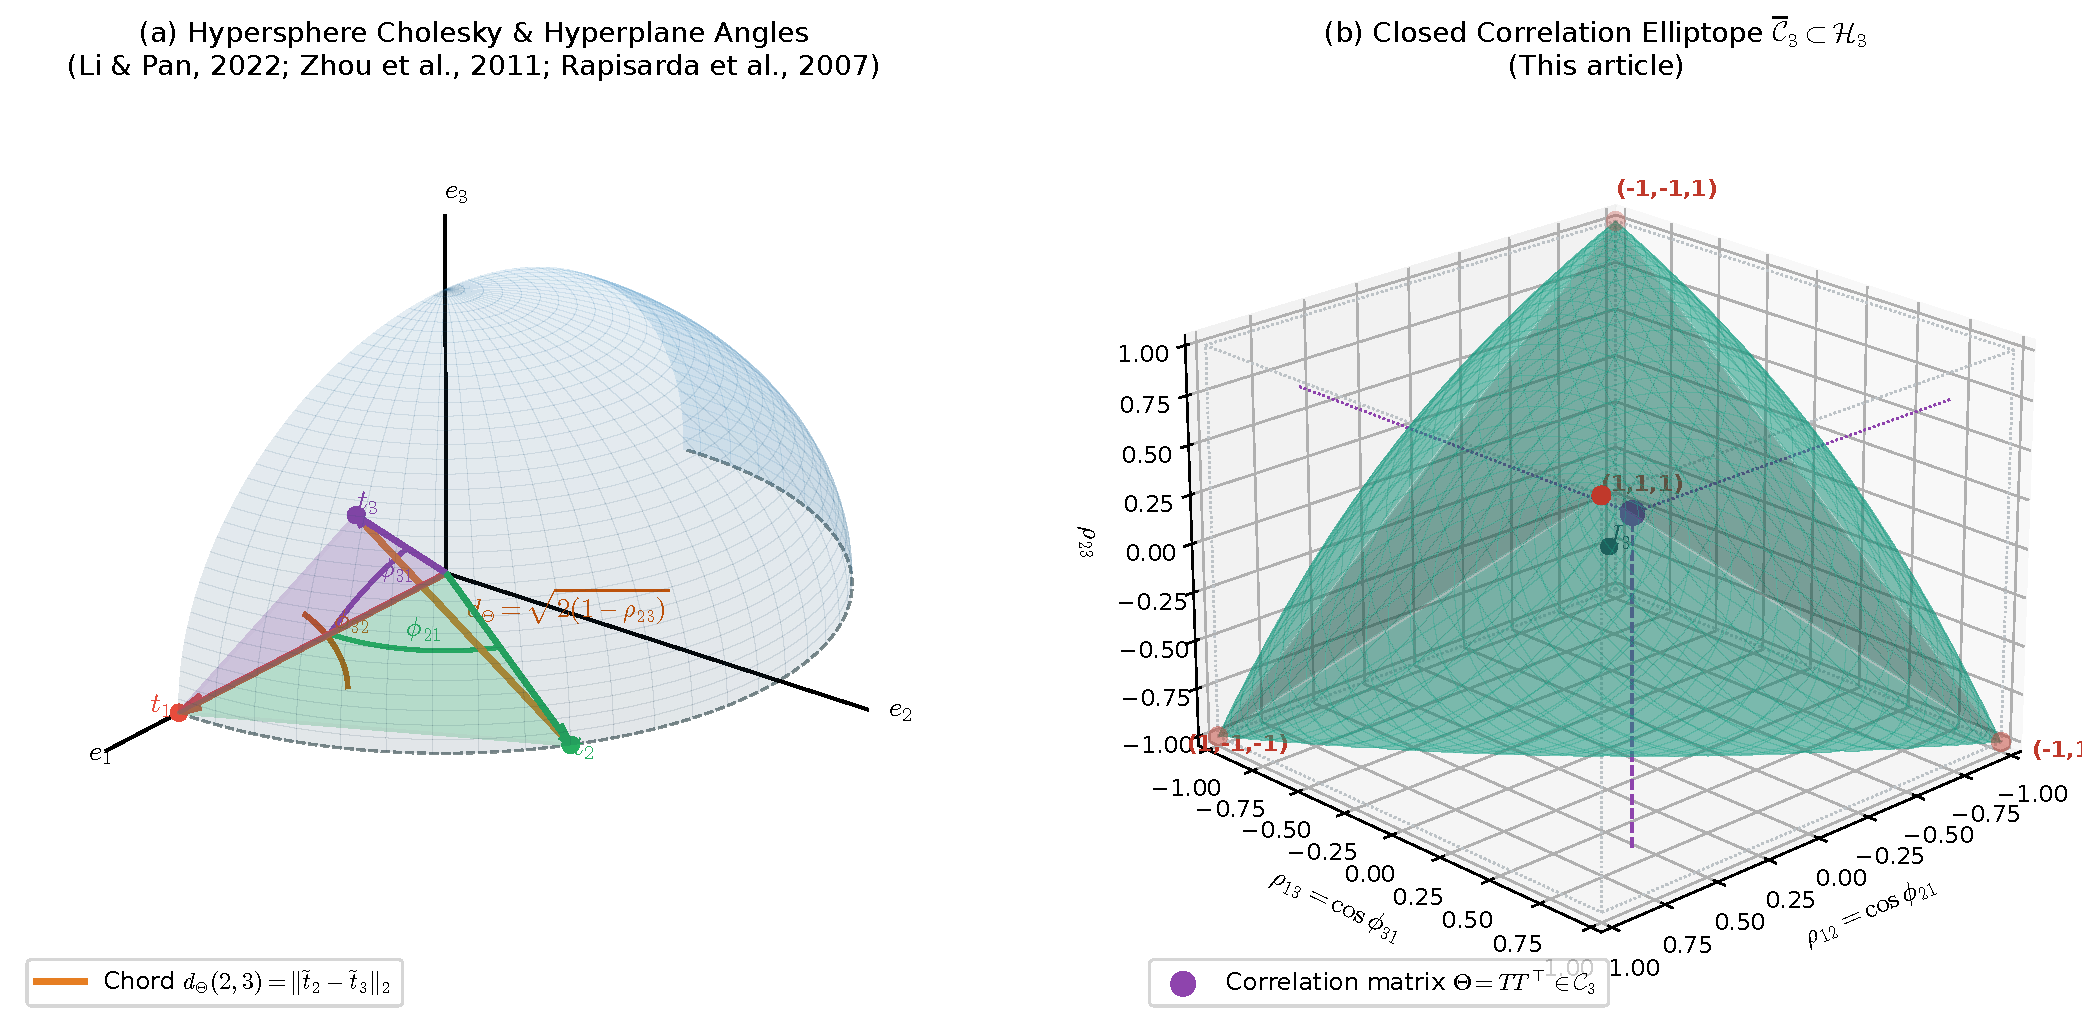
\includegraphics[width=\textwidth]{figures/fig0_geometry_elliptope.pdf}
\caption{Complementary geometric representations of qualitative correlation structures: the Cholesky hypersphere embedding and the closed 3D correlation elliptope $\overline{\mathcal{C}}_3$. 
(a) Representation of qualitative levels as unit vectors $t_1, t_2, t_3$ on the Cholesky hemisphere $\mathbb{S}^2_+$ \citep{Zhou,HS_Jacobi,li2022permutation}, where $\phi_{21}$ and $\phi_{31}$ are spherical angles, $\phi_{32}$ is the dihedral angle between hyperplanes $HP_{12}$ and $HP_{13}$, and the distance $d_\Theta(2, 3) = \sqrt{2(1 - \rho_{23})}$ is the Euclidean chord length $\|\widetilde{t}_2 - \widetilde{t}_3\|_2$. 
(b) The closed 3D correlation elliptope $\overline{\mathcal{C}}_3 \subset [-1, 1]^3$ defined by $\det(\Theta) \ge 0$ and $|\rho_{jk}| \le 1$, showing the four rank-1 singular vertices of $\overline{\mathcal{C}}_3$ ($\rho_{12}\rho_{13}\rho_{23} = 1$), the origin $I_3$, and the interior correlation matrix $\Theta = T T^\top \in \mathcal{C}_3$ corresponding to panel~(a).}
\label{fig:elliptope_geometry}
\end{figure}

To tackle the curse of dimensionality, supervised dimension reduction aims to compress the high-dimensional parameter space $\mathbb{R}^{D_{\inp}}$ onto a low-dimensional latent elliptope $\mathcal{C}_\ell$ with $\ell \ll L$, depending only on $D_{\outp} := \frac{1}{2}\ell(\ell - 1) \ll D_{\inp}$ hyperparameters.
However, by analogy with projection-based model order reduction where linear interpolation of local operators fails to preserve the Riemannian manifold geometry of symmetric positive definite matrices~\citep{porrello2024bayesian}, linear transformations between the correlation elliptopes $\mathcal{S}_1^\ell$ and $\mathcal{S}_1^L$ do not automatically preserve positive definiteness on non-polyhedral spectrahedral domains.
This motivates the formal construction of the transformation operators below and their spectral characterization in Section~\ref{sec:theorems}.


\subsection{Cross-Level Indicator Encoding and Index Bijection}
\label{sec:crosslevel}
To link discrete level observations to the pairwise correlation parameter space $\mathbb{R}^{D_{\inp}}$, we build upon and recall the cross-level indicator relaxation originally introduced in an engineering context by \citet{saves2023high}, and establish its formal matrix-theoretic and algebraic properties. Specifically, this subsection formalizes the indicator encoding connecting categorical input levels to correlation coordinates, and establishes the bidirectional operators. The latter is used to navigate between the reduced latent space and the full parameter space, effectively tracking the qualitative input domain through its induced correlation parameters~\citep{Mixed_Paul}.

\begin{definition}[Lexicographical index bijection $\psi$]
\label{def:psi}
For any integer $n \ge 2$, let $\mathcal{I}_n = \{ (k, k') : 1 \le k < k' \le n \}$. The lexicographical mapping $\psi(\cdot, \cdot, n) : \mathcal{I}_n \to \{1, \ldots, D(n)\}$ is defined by:
\begin{equation}
\label{eq:psi_formula}
\psi(k, k', n) = \frac{1}{2}\left( (n-1)(n-2) - (n-k)(n-k-1) \right) + k' - 1.
\end{equation}
The mapping $\psi(\cdot, \cdot, n)$ is a bijection enumerating the upper-triangular pairs row by row. Its inverse is denoted $\psi^{-1}(\cdot, n) : \{1, \ldots, D(n)\} \to \mathcal{I}_n$.
\end{definition}

\begin{definition}[Cross-level indicator relaxation]
\label{def:cross_level}
For an observed categorical level $c \in \{1, \ldots, L\}$, the cross-level indicator vector $\zeta_c \in \{0, 1\}^{D_{\inp}}$ is defined coordinate-wise for each $m \in \{1, \ldots, D_{\inp}\}$ by:
\begin{equation}
[\zeta_c]_m =
\begin{cases}
1, & \text{if } j = c \text{ or } j' = c, \text{ where } (j, j') = \psi^{-1}(m, L), \\
0, & \text{otherwise.}
\end{cases}
\end{equation}
The vector $\zeta_c$ contains exactly $L-1$ ones and $D_{\inp} - (L - 1)$ zeros, indicating all pairwise correlations in which level $c$ participates.
\end{definition}

\begin{lemma}[from~\citep{saves2023high}]
\label{lem:hadamard}
Let $c, c' \in \{1, \ldots, L\}$ with $c \neq c'$. The Hadamard (element-wise) product $\zeta_c \odot \zeta_{c'} \in \{0, 1\}^{D_{\inp}}$ satisfies:
\begin{equation}
\label{eq:hadamard_select}
[\zeta_c \odot \zeta_{c'}]_m =
\begin{cases}
1, & \text{if } m = \psi(\min(c, c'),\, \max(c, c'),\, L), \\
0, & \text{otherwise.}
\end{cases}
\end{equation}
Consequently, $\zeta_c \odot \zeta_{c'} = e_{m^*}$, the canonical basis vector in $\mathbb{R}^{D_{\inp}}$ associated with the pair $\{c, c'\}$.
\end{lemma}

\begin{proof}
Immediate from Definition~\ref{def:cross_level}: for $c \neq c'$, $\{c, c'\}$ is the unique unordered pair containing both categorical levels, indexed bijectively by $m^* = \psi(\min(c, c'), \max(c, c'), L)$, while all other coordinates vanish.
\end{proof}


Let $c_1, \ldots, c_{n_t} \in \{1, \ldots, L\}$ with $L \ge 3$ be $n_t$ categorical observations with one-hot assignment matrix $M \in \{0, 1\}^{n_t \times L}$ ($L_{\mathrm{obs}}$ observed levels). Let $E \in \{0, 1\}^{L \times D_{\inp}}$ denote the unoriented vertex-edge incidence matrix of the complete graph $K_L$, whose $j$-th row is the cross-level indicator vector $\zeta_j^\top$.
\begin{enumerate}[(a)]
    \item[(a)] \textbf{Incidence Gram identity and isometry on $\mathds{1}_L^\perp$:} The design matrix factors as $X = M E \in \mathbb{R}^{n_t \times D_{\inp}}$, and the incidence matrix satisfies the classical complete-graph identity \citep[Section~8.2]{godsil2001algebraic}:
    \begin{equation}
    \label{eq:incidence_gram}
    E E^\top = (L - 2) I_L + \mathds{1}_L \mathds{1}_L^\top.
    \end{equation}
    Its spectrum consists of $\lambda_1(E E^\top) = 2(L - 1)$ (multiplicity $1$, eigenvector $\mathds{1}_L$) and $\lambda_2 = \cdots = \lambda_L = L - 2$ on the centered subspace $\mathds{1}_L^\perp$. Consequently, for any $u \in \mathds{1}_L^\perp$, $E^\top$ is an exact homothety with $\|E^\top u\|_2 = \sqrt{L - 2} \|u\|_2$, establishing $\rank(E) = L$.
    \item[(b)] \textbf{Exact column rank of centered design $\tilde{X}$:} Centering $X$ via $H_{n_t} = I_{n_t} - \frac{1}{n_t}\mathds{1}_{n_t}\mathds{1}_{n_t}^\top$ yields $\tilde{X} = H_{n_t} M E$, whose covariance Gram matrix satisfies:
    \begin{equation}
    \label{eq:centered_gram_factor}
    \tilde{X} \tilde{X}^\top = (L - 2) H_{n_t} M M^\top H_{n_t},
    \end{equation}
    with exact column rank $\rank(\tilde{X}) = L_{\mathrm{obs}} - 1 \le \min(n_t - 1, L - 1)$.
    \item[(c)] \textbf{Krylov subspace degeneracy in non-mixed cases:} When observations are purely categorical and balanced ($n_j = n_t / L$ for all $j$), $\tilde{X}\tilde{X}^\top = \frac{n_t}{L}(L - 2) M H_L M^\top$ has a single distinct non-zero eigenvalue $\frac{n_t}{L}(L - 2)$ of multiplicity $L - 1$. Consequently, the univariate PLS Krylov subspace $\mathcal{K}_m(\tilde{X}^\top \tilde{X}, \tilde{X}^\top \tilde{\bm{y}})$ is 1-dimensional, terminating in a single step ($D_{\outp} = 1$). To extract $D_{\outp} = \frac{1}{2}\ell(\ell-1) \ge 2$ informative directions without Krylov breakdown ($D_{\outp} \le L_{\mathrm{obs}} - 1$), PLS requires coupling with continuous covariates (as in mixed KPLS) or hierarchical categorical groupings.
\end{enumerate}

\begin{proof}[Proof sketch]
For (a), following algebraic graph theory \citep{godsil2001algebraic}, row $j$ of $E$ has entry $1$ for each of the $L-1$ edges incident to vertex $j$, so $[E E^\top]_{j, j} = L - 1$. For $j \neq j'$, the pair $\{j, j'\}$ forms a unique edge in $K_L$, so $[E E^\top]_{j, j'} = 1$. Thus $E E^\top = (L - 1)I_L + (\mathds{1}_L\mathds{1}_L^\top - I_L) = (L - 2)I_L + \mathds{1}_L\mathds{1}_L^\top$. For $u \perp \mathds{1}_L$, $E E^\top u = (L - 2)u$, so $\|E^\top u\|_2^2 = (L - 2)\|u\|_2^2$. For $L \ge 3$, $L - 2 > 0$ and $2(L - 1) > 0$, proving $\rank(E) = L$. For (b), $X = M E$ implies $\tilde{X}\tilde{X}^\top = H_{n_t} M E E^\top M^\top H_{n_t}$. Since $M \mathds{1}_L = \mathds{1}_{n_t}$ and $H_{n_t} \mathds{1}_{n_t} = \bm{0}$, the term $\mathds{1}_L \mathds{1}_L^\top$ vanishes, establishing Eq.\eqnref{eq:centered_gram_factor}. Since $E$ has full row rank $L$, $\rank(\tilde{X}) = \rank(H_{n_t} M) = L_{\mathrm{obs}} - 1$. For (c), in balanced designs $M^\top M = \frac{n_t}{L} I_L$, deflating residual Krylov directions $m \ge 2$. Complete algebraic details are in Appendix~\ref{subsec:proof_rank_bound}.
\end{proof}
Proposition (c) establishes that in an uncoupled, purely categorical balanced design with no continuous variation, the covariance operator collapses onto a single non-trivial eigenspace, rendering higher-order categorical Krylov directions uninformative. In mixed-variable GP emulation as implemented in the Surrogate Modeling Toolbox (SMT) and evaluated in the benchmarks, this degeneracy is naturally eliminated. The PLS regression is performed on the joint mixed design matrix:
\begin{equation}
\label{eq:joint_pls_matrix}
X_{\mathrm{joint}} = \begin{bmatrix} X_{\mathrm{quant}} & X_{\mathrm{cat}} \end{bmatrix} \in \mathbb{R}^{n_t \times (d + D_{\inp})}.
\end{equation}
While empirical column standardization scales all categorical columns of $X_{\mathrm{cat}}$ by an identical factor in balanced designs ($n_j = n_t/L$), the continuous inputs $x \in \mathbb{R}^d$ couple with the response variation across distinct categorical levels. Specifically, because the global Latin Hypercube Sampling (LHS) design induces non-zero sample cross-covariances $\tilde{X}_{\mathrm{cat}}^\top \tilde{X}_{\mathrm{quant}} \neq \bm{0}$ across levels, the joint covariance $\tilde{X}_{\mathrm{joint}}^\top \tilde{X}_{\mathrm{joint}}$ breaks the invariant eigenspace homothety of $\tilde{X}_{\mathrm{cat}}^\top \tilde{X}_{\mathrm{cat}}$. Because $\rank(\tilde{X}_{\mathrm{cat}}) = L_{\mathrm{obs}} - 1$ by Proposition~(b), concatenating $d$ continuous design columns yields the sharp rank bound:
\begin{equation}
\label{eq:krylov_bound}
\dim \mathcal{K}_m(\tilde{X}_{\mathrm{joint}}^\top \tilde{X}_{\mathrm{joint}}, \tilde{X}_{\mathrm{joint}}^\top \tilde{\bm{y}}) \le \rank(\tilde{X}_{\mathrm{joint}}) \le \min(n_t - 1, d + L_{\mathrm{obs}} - 1).
\end{equation}
    Equality holds generically whenever the continuous design columns are linearly independent, the centered joint covariance matrix $\tilde{X}_{\mathrm{joint}}^\top \tilde{X}_{\mathrm{joint}}$ possesses mutually distinct non-zero eigenvalues, and the initial PLS projection vector $\tilde{X}_{\mathrm{joint}}^\top \tilde{\bm{y}}$ is not orthogonal to any invariant eigenspace. To ensure that $D_{\outp} = \frac{1}{2}\ell(\ell-1)$ non-degenerate latent directions can be extracted without Krylov rank starvation, the mixed problem must satisfy $d + L_{\mathrm{obs}} - 1 \ge D_{\outp}$. 
    In mixed-variable settings ($d \ge 1$), continuous and categorical columns are standardized before decomposition, allowing PLS to extract non-degenerate orthogonal components with non-vanishing weight norms, fully eliminating the 1-dimensional Krylov degeneracy.
    Let $G_{\mathrm{PLS}}, \Xi_{\mathrm{PLS}} \in \mathbb{R}^{(d+D_{\inp}) \times D_{\outp}}$ denote the joint PLS weight and loading matrices, respectively. From the joint rotation matrix $G_{\mathrm{joint}} = G_{\mathrm{PLS}}(\Xi_{\mathrm{PLS}}^\top G_{\mathrm{PLS}})^{-1}$, the raw categorical submatrix $G_*^{\mathrm{raw}} = [G_{\mathrm{joint}}]_{d+1:d+D_{\inp}, \cdot} \in \mathbb{R}^{D_{\inp} \times D_{\outp}}$ is extracted and row-normalized to yield the valid unit-row-norm reconstruction weights $G_* \in \mathbb{R}^{D_{\inp} \times D_{\outp}}$ for all $D_{\outp} = \frac{1}{2}\ell(\ell-1)$ latent dimensions.

  
\begin{definition}[Reconstruction operator $\mathcal{T}_{G_*}$]
\label{def:operator}
Let $G_* \in \mathbb{R}^{D_{\inp} \times D_{\outp}}$. The reconstruction operator $\mathcal{T}_{G_*} : \mathcal{S}_1^\ell \to \mathcal{S}_1^L$ maps a reduced symmetric matrix $\hat{\Theta} \in \mathcal{S}_1^\ell$ to an $L \times L$ symmetric matrix $\Theta = \mathcal{T}_{G_*}(\hat{\Theta}) \in \mathcal{S}_1^L$ defined as follows.
\begin{enumerate}
    \item Unit diagonal: $[\Theta]_{j, j} = 1$ for all $j \in \{1, \ldots, L\}$.
    \item Off-diagonal entries: $\forall \ 1 \le j < j' \le L$,
    \begin{equation}
    \label{eq:recon_formula}
    [\mathcal{T}_{G_*}(\hat{\Theta})]_{j, j'} = \sum_{t=1}^{\ell} \sum_{t'=t+1}^{\ell} \left( [G_*]_{\psi(j,j',L), \psi(t,t',\ell)} \right)^2 [\hat{\Theta}]_{t, t'}.
    \end{equation}
    \item Symmetry: $[\Theta]_{j', j} = [\Theta]_{j, j'}$ for all $1 \le j < j' \le L$.
\end{enumerate}
\end{definition}

\begin{definition}[Reduction operator $\mathcal{R}_W$]
\label{def:reduction_op}
Let $W \in \mathbb{R}^{D_{\outp} \times D_{\inp}}$ be a non-negative row-stochastic matrix, meaning that $[W]_{p, r} \ge 0$ for all $p \in \{1, \ldots, D_{\outp}\}$ and $r \in \{1, \ldots, D_{\inp}\}$, with row sums satisfying:
\begin{equation}
\label{eq:row_stochastic}
\sum_{r=1}^{D_{\inp}} [W]_{p, r} = 1, \quad \forall p \in \{1, \ldots, D_{\outp}\}.
\end{equation}
The reduction operator $\mathcal{R}_W : \mathcal{S}_1^L \to \mathcal{S}_1^\ell$ maps an $L \times L$ symmetric matrix $\Theta \in \mathcal{S}_1^L$ to an $\ell \times \ell$ symmetric matrix $\hat{\Theta} = \mathcal{R}_W(\Theta) \in \mathcal{S}_1^\ell$ defined as follows.
\begin{enumerate}
    \item Unit diagonal: $[\hat{\Theta}]_{t, t} = 1$ for all $t \in \{1, \ldots, \ell\}$.
    \item Off-diagonal entries:  $ \forall \  1 \le t < t' \le \ell$, setting row index $p = \psi(t, t', \ell) \in \{1, \ldots, D_{\outp}\}$,
    \begin{equation}
    \label{eq:reduc_formula}
    [\mathcal{R}_W(\Theta)]_{t, t'} = \sum_{j=1}^L \sum_{j'=j+1}^L [W]_{p, \psi(j,j',L)} \, [\Theta]_{j, j'}.
    \end{equation}
    \item Symmetry: $[\hat{\Theta}]_{t', t} = [\hat{\Theta}]_{t, t'}$ for all $1 \le t < t' \le \ell$.
\end{enumerate}
\end{definition}
In practice, while GP use the reconstruction operator $\mathcal{T}_{G_*}$ to map latent parameters into the full correlation space during inference, the adjoint reduction operator $\mathcal{R}_W$ provides a practical computational capability: it enables an instantaneous, closed-form projection to \textit{warm-start} profile likelihood optimization~\citep{saves2023high}.
Specifically, if a full-space prior or empirical correlation matrix $\Theta_{\mathrm{prior}}$ is available (from physical domain knowledge, nominal configurations, or exploratory inter-level empirical response correlations $\Theta_{\mathrm{emp}}$), setting $\hat{\Theta}_0 = \mathcal{R}_W(\Theta_{\mathrm{prior}}) \in \mathcal{H}_\ell$ provides a fast, non-iterative initial point in the reduced latent space whose entries are guaranteed to reside in $[-1, 1]$ by convex combination~\citep{Abramson2002,van2024reference}. Because linear reduction does not automatically preserve positive definiteness for arbitrary full-space matrices, positive definiteness is certified by checking $\lambda_{\min}(\hat{\Theta}_0)$; if non-positive, a trivial $O(\ell^2)$ diagonal repair on the small $\ell \times \ell$ matrix ($\approx 16$ for $\ell=4$) restores $\hat{\Theta}_0 \in \mathcal{C}_\ell$ before initiating optimization. 


\subsection{The Unit Row-Norm Condition and the Row-Normalized PLS (RN-PLS) Model}

The PLS rotation matrix $G_* \in \mathbb{R}^{D_{\inp} \times D_{\outp}}$ satisfies: for every row index $r \in \{1, \ldots, D_{\inp}\}$,
\begin{equation}
\label{eq:unit_row_norm}
\omega_r \;:=\; \sum_{p=1}^{D_{\outp}} \left( [G_*]_{r, p} \right)^2 = 1.
\end{equation}
In the general case, this unit row assumption can always be enforced with a simple renormalization. Equivalently, every row vector of $G_*$ has unit Euclidean norm: $\|[G_*]_{r, \cdot}\|_2 = 1$.
% 
In standard PLS regression, the categorical submatrix $G_*^{\mathrm{raw}} = [G_{\mathrm{PLS}}(\Xi_{\mathrm{PLS}}^\top G_{\mathrm{PLS}})^{-1}]_{d+1:d+D_{\inp},\cdot}$ does not possess unit row norms in general \citep{wold_1975,hellandStructurePartialLeast1988,bouhlel_KPLSK,Bouhlel18}. Row norms $\sqrt{\omega_r}$ in raw PLS can vary widely (\textit{e.g.}, from $0.01$ to $4.9$ for $L=20$), causing unnormalized reconstruction weights $\sum_{p=1}^{D_{\outp}} ([G_*^{\mathrm{raw}}]_{r,p})^2$ to fluctuate by up to two orders of magnitude and driving reconstructed correlations far outside $[-1, 1]$.

\begin{equation}
\label{eq:row_normalization}
[G_*]_{r, p} =
\begin{cases}
\displaystyle\frac{[G_*^{\mathrm{raw}}]_{r, p}}{\sqrt{\omega_r}}, & \text{if } \omega_r = \sum_{p'=1}^{D_{\outp}} \left([G_*^{\mathrm{raw}}]_{r, p'}\right)^2 > 0, \\[8pt]
\displaystyle\frac{1}{\sqrt{D_{\outp}}}, & \text{if } \omega_r = 0,
\end{cases}
\end{equation}
where the convention for $\omega_r = 0$ handles the uninformative boundary case when a categorical pair is unobserved in the training sample, assigning equal prior weight across latent coordinates while strictly preserving the unit Euclidean norm $\|[G_*]_{r, \cdot}\|_2 = 1$.
Importantly, row normalization applies non-uniform scalings across different pairs $\{j, j'\}$, reweighting the relative importance of each pairwise correlation coordinate. RN-PLS should therefore be understood as a structurally constrained projection architecture designed specifically to guarantee convex combination weights on the correlation elliptope, rather than as an exact reparameterization of unconstrained PLS.

Furthermore, whenever all $D_{\outp} = \frac{1}{2}\ell(\ell-1)$ pairwise latent correlation coordinates are informative and active, meaning that every column of $G_*$ is non-zero, satisfying $\sum_{r'=1}^{D_{\inp}} ([G_*]_{r', p})^2 > 0$ for all $p \in \{1, \ldots, D_{\outp}\}$, the canonical adjoint row-stochastic reduction matrix $W \in \mathbb{R}^{D_{\outp} \times D_{\inp}}$ is given in closed form by:
\begin{equation}
\label{eq:W_definition}
[W]_{p, r} = \frac{\left([G_*]_{r, p}\right)^2}{\sum_{r'=1}^{D_{\inp}} \left([G_*]_{r', p}\right)^2}, \quad \forall p \in \{1, \ldots, D_{\outp}\}, \; r \in \{1, \ldots, D_{\inp}\},
\end{equation}
ensuring that $\sum_{r=1}^{D_{\inp}} [W]_{p, r} = 1$ and each reduced latent correlation is an exact convex combination of full-space correlations.
    
\begin{lemma}
\label{lem:convex}\label{lem:entry_bound}\label{th:entry_bound}\label{lem:convex_bound}
Under unit row norm assumption, for any $(j, j') \in \mathcal{I}_L$, the reconstruction weights defined by:
\begin{equation}
\label{eq:weights}
w_{(j,j')}^{(t,t')} := \left( [G_*]_{\psi(j,j',L), \psi(t,t',\ell)} \right)^2, \quad \forall (t, t') \in \mathcal{I}_\ell,
\end{equation}
satisfy $w_{(j,j')}^{(t,t')} \ge 0$ and $\sum_{(t,t') \in \mathcal{I}_\ell} w_{(j,j')}^{(t,t')} = 1$. Consequently:
\begin{enumerate}
    \item[(a)] Every off-diagonal entry $[\mathcal{T}_{G_*}(\hat{\Theta})]_{j, j'}$ is a convex combination of the latent off-diagonal entries $\{ [\hat{\Theta}]_{t, t'} : (t, t') \in \mathcal{I}_\ell \}$.
    \item[(b)] The operators preserve the correlation hypercube: $\mathcal{T}_{G_*}(\mathcal{H}_\ell) \subseteq \mathcal{H}_L$ and $\mathcal{R}_W(\mathcal{H}_L) \subseteq \mathcal{H}_\ell$.
\end{enumerate}
\end{lemma}

\begin{proof}
Non-negativity holds because each weight is the square of a real number. For (a), let $r = \psi(j, j', L)$. Because $\psi(\cdot, \cdot, \ell)$ is a bijection from $\mathcal{I}_\ell$ to $\{1, \ldots, D_{\outp}\}$, re-indexing yields $\sum_{(t,t')} w_{(j,j')}^{(t,t')} = \sum_{p=1}^{D_{\outp}} ([G_*]_{r, p})^2 = \omega_r = 1$ by unit row norm assumption. For (b), by the triangle inequality, $|[\Theta]_{j, j'}| \le \sum_{(t,t')} w_{(j,j')}^{(t,t')} |[\hat{\Theta}]_{t, t'}| \le \sum_{(t,t')} w_{(j,j')}^{(t,t')} \cdot 1 = 1$, with unit diagonals preserved by definition. The same convex combination bound applies to $\mathcal{R}_W$ via the row-stochasticity of $W$.
\end{proof}


Let the unit row norm assumption hold with latent dimension $\ell = 2$, so that the latent correlation space has dimension $D_{\outp} = \frac{1}{2}(2)(1) = 1$. Suppose every row of $G_*^{\mathrm{raw}}$ is non-zero ($\omega_r > 0$). Then:
\begin{enumerate}
    \item[(a)] \textbf{Trivial row weights:} For every coordinate $r \in \{1, \ldots, D_{\inp}\}$, the normalized rotation matrix satisfies:
    \begin{equation}
    \label{eq:l2_weight_trivial}
    \left([G_*]_{r, 1}\right)^2 \equiv 1.
    \end{equation}
    \item[(b)] \textbf{Collapse to equicorrelation:} For any latent correlation matrix $\hat{\Theta} = \begin{pmatrix} 1 & \rho \\ \rho & 1 \end{pmatrix} \in \mathcal{C}_2$ parameterized by scalar $\rho \in (-1, 1)$, the reconstructed matrix $\Theta = \mathcal{T}_{G_*}(\hat{\Theta}) \in \mathcal{S}_1^L$ collapses identically to the uniform equicorrelation matrix:
    \begin{equation}
    [\mathcal{T}_{G_*}(\hat{\Theta})]_{j, j'} = \rho \quad \forall 1 \le j < j' \le L, \quad \text{i.e., } \Theta = (1 - \rho) I_L + \rho \mathds{1}_L \mathds{1}_L^\top.
    \end{equation}
    \item[(c)] \textbf{Erasure of the PLS projection:} The reconstructed matrix $\mathcal{T}_{G_*}(\hat{\Theta})$ is invariant to the cross-level design matrix $X$, the response vector $y$, and the raw PLS rotation matrix $G_*^{\mathrm{raw}}$.
\end{enumerate}
Consequently, for RN-PLS to perform non-trivial, data-driven differential weighting across correlation coordinates, a necessary mathematical condition is $D_{\outp} \ge 2$, which strictly requires $\ell \ge 3$. Even though this result is simple and direct, it connects RN-PLS back to the model hierarchy established in~\citep{Mixed_Paul}.

\begin{proof}
For (a), when $\ell=2$, $D_{\outp}=1$, so $G_*^{\mathrm{raw}} \in \mathbb{R}^{D_{\inp} \times 1}$ has a single column. The row norm is $\sqrt{\omega_r} = |[G_*^{\mathrm{raw}}]_{r, 1}|$. Dividing by $\sqrt{\omega_r}$ yields $[G_*]_{r, 1} = \operatorname{sgn}\bigl([G_*^{\mathrm{raw}}]_{r, 1}\bigr) \in \{-1, +1\}$, so $([G_*]_{r, 1})^2 \equiv 1$ for all $r \in \{1, \ldots, D_{\inp}\}$.
For (b), substituting $([G_*]_{r, 1})^2 = 1$ into Definition~\ref{def:operator} yields $[\mathcal{T}_{G_*}(\hat{\Theta})]_{j, j'} = 1 \cdot [\hat{\Theta}]_{1, 2} = \rho$ for all $j < j'$.
For (c), because $([G_*]_{r, 1})^2 \equiv 1$ regardless of the numerical entries of $G_*^{\mathrm{raw}}$, all data information captured by PLS is identically canceled by the unit row normalization. To obtain non-trivial convex combination weights where $\sum_{p=1}^{D_{\outp}} ([G_*]_{r, p})^2 = 1$ with $[G_*]_{r, p}^2 \not\equiv 1$, we must have $D_{\outp} \ge 2 \iff \frac{1}{2}\ell(\ell-1) \ge 2 \iff \ell \ge 3$.
\end{proof}

\begin{theorem}
\label{th:roundtrip_contraction}
Let the unit row norm assumption hold with active columns $d_p = \sum_{r=1}^{D_{\inp}} ([G_*]_{r, p})^2 > 0$ for all $p \in \{1, \dots, D_{\outp}\}$. Let $A := G_* \odot G_* \in \mathbb{R}_{\ge 0}^{D_{\inp} \times D_{\outp}}$ denote the reconstruction weight matrix, $D_{\mathrm{col}} := \diag(d_1, \dots, d_{D_{\outp}})$, and let $W = D_{\mathrm{col}}^{-1} A^\top \in \mathbb{R}^{D_{\outp} \times D_{\inp}}$ be the canonical row-stochastic adjoint matrix defined in Eq.\eqnref{eq:W_definition}. Consider the round-trip composite operator $\mathcal{P} := \mathcal{R}_W \circ \mathcal{T}_{G_*} : \mathcal{S}_1^\ell \to \mathcal{S}_1^\ell$.
\begin{enumerate}[(a)]
    \item[(a)] \textbf{Matrix factorization, reversibility, and stationary distribution:} For any $\hat{\Theta} \in \mathcal{S}_1^\ell$ with off-diagonal vector $\hat{\bm{\theta}} = (\theta_1, \dots, \theta_{D_{\outp}})^\top$, the composite operator acts linearly on the off-diagonal entries:
    \begin{equation}
    \label{eq:roundtrip_matrix}
    \operatorname{vec}_{\mathrm{off}}\bigl(\mathcal{P}(\hat{\Theta})\bigr) = M \hat{\bm{\theta}}, \quad \text{where } M := W A = D_{\mathrm{col}}^{-1} A^\top A \in \mathbb{R}^{D_{\outp} \times D_{\outp}}.
    \end{equation}
    The transition matrix $M$ is row-stochastic ($M \mathds{1}_{D_{\outp}} = \mathds{1}_{D_{\outp}}$) and reversible with respect to $D_{\mathrm{col}}$, satisfying detailed balance:
    \begin{equation}
    \label{eq:detailed_balance}
    D_{\mathrm{col}} M = A^\top A = M^\top D_{\mathrm{col}}.
    \end{equation}
    A stationary distribution is given explicitly in closed form by:
    \begin{equation}
    \label{eq:stationary_pi}
    \bm{\pi} = \frac{1}{D_{\inp}} \bm{d} = \frac{1}{D_{\inp}} (d_1, \dots, d_{D_{\outp}})^\top \in \Delta_{D_{\outp}}, \quad \text{with } \bm{\pi}^\top M = \bm{\pi}^\top,
    \end{equation}
    which is unique whenever the Markov chain induced by $M$ is irreducible.
    \item[(b)] \textbf{Entirely real positive semidefinite spectrum in $[0, 1]$:} The transition matrix $M$ is similar to the symmetric positive semidefinite matrix:
    \begin{equation}
    \label{eq:sym_markov_S}
    S := D_{\mathrm{col}}^{1/2} M D_{\mathrm{col}}^{-1/2} = D_{\mathrm{col}}^{-1/2} A^\top A D_{\mathrm{col}}^{-1/2} = (A D_{\mathrm{col}}^{-1/2})^\top (A D_{\mathrm{col}}^{-1/2}) \succeq 0.
    \end{equation}
    Consequently, all $D_{\outp}$ eigenvalues of $M$ are strictly real, non-negative, and bounded by 1:
    \begin{equation}
    0 \le \lambda_{D_{\outp}}(M) \le \dots \le \lambda_2(M) \le \lambda_1(M) = 1.
    \end{equation}
    In particular, $M$ possesses no complex conjugate eigenvalues, no oscillatory modes, no defective Jordan blocks, and is diagonalizable in $\mathbb{R}$.
    \item[(c)] \textbf{Preservation of reconstructed full-space mean correlation:} For any latent correlation vector $\hat{\bm{\theta}} \in \mathbb{R}^{D_{\outp}}$, the arithmetic mean of all $D_{\inp}$ reconstructed pairwise correlations $\bm{\theta}_{\mathrm{full}} = A \hat{\bm{\theta}} \in \mathbb{R}^{D_{\inp}}$ satisfies:
    \begin{equation}
    \label{eq:mean_preservation}
    \bar{\theta}_{\mathrm{full}} := \frac{1}{D_{\inp}} \sum_{r=1}^{D_{\inp}} [\bm{\theta}_{\mathrm{full}}]_r = \frac{1}{D_{\inp}} \mathds{1}_{D_{\inp}}^\top A \hat{\bm{\theta}} = \bm{\pi}^\top \hat{\bm{\theta}}.
    \end{equation}
    This reconstructed full-space mean is an exact invariant under the round-trip operator: $\bm{\pi}^\top (M \hat{\bm{\theta}}) = \bm{\pi}^\top \hat{\bm{\theta}} = \bar{\theta}_{\mathrm{full}}$.
    \item[(d)] \textbf{Geometric convergence to equicorrelation:} If the Markov chain induced by $M$ is irreducible, the second eigenvalue satisfies $\lambda_2(M) < 1$. Under iterated round-trip projections $\mathcal{P}^k$, the latent correlations converge geometrically to the uniform equicorrelation matrix $\hat{\Theta}(\bar{\theta}_{\mathrm{full}})$:
    \begin{equation}
    \lim_{k \to \infty} M^k \hat{\bm{\theta}} = \bar{\theta}_{\mathrm{full}} \mathds{1}_{D_{\outp}},
    \end{equation}
    with contraction rate governed by the spectral gap $1 - \lambda_2(M)$:
    \begin{equation}
    \|M^k \hat{\bm{\theta}} - \bar{\theta}_{\mathrm{full}} \mathds{1}_{D_{\outp}}\|_{D_{\mathrm{col}}} \le \lambda_2(M)^k \|\hat{\bm{\theta}} - \bar{\theta}_{\mathrm{full}} \mathds{1}_{D_{\outp}}\|_{D_{\mathrm{col}}},
    \end{equation}
    where $\|v\|_{D_{\mathrm{col}}} = \sqrt{v^\top D_{\mathrm{col}} v} = \sqrt{D_{\inp}} \|v\|_{\bm{\pi}}$.
    \item[(e)] \textbf{Dobrushin ergodic oscillation non-expansion:} For single-step coordinate dispersion $\operatorname{spread}(\hat{\bm{\theta}}) := \max_p \hat{\theta}_p - \min_p \hat{\theta}_p$, the unconditional non-expansion bound holds:
    \begin{equation}
    \operatorname{spread}(M \hat{\bm{\theta}}) \le \tau(M) \operatorname{spread}(\hat{\bm{\theta}}),
    \end{equation}
    where $\tau(M) = 1 - \min_{p, p'} \sum_{q=1}^{D_{\outp}} \min([M]_{p, q}, [M]_{p', q}) = \frac{1}{2} \max_{p, p'} \sum_{q=1}^{D_{\outp}} |[M]_{p, q} - [M]_{p', q}| \le 1$ is Dobrushin's ergodic coefficient of $M$ \citep{dobrushin1956,seneta2006non}, with strict single-step contraction ($\tau(M) < 1$) holding if and only if $M$ satisfies Dobrushin's scrambling condition.
\end{enumerate}
\end{theorem}

\begin{proof}[Proof sketch]
For (a), the matrix identity $M = D_{\mathrm{col}}^{-1} A^\top A$ follows from Definitions~\ref{def:reduction_op} and~\ref{def:operator}, with row-stochasticity and detailed balance $D_{\mathrm{col}} M = M^\top D_{\mathrm{col}}$ following from $A \mathds{1} = \mathds{1}$. For (b), similarity to the symmetric Gram matrix $S = D_{\mathrm{col}}^{-1/2} A^\top A D_{\mathrm{col}}^{-1/2}$ establishes real non-negative eigenvalues in $[0, 1]$. Property (c) follows from $\bm{\pi}^\top M = \bm{\pi}^\top$. Properties (d) and (e) follow from the spectral gap $\lambda_2(M) < 1$ in the weighted norm $\|\cdot\|_{D_{\mathrm{col}}}$ and Dobrushin's ergodic coefficient for Markov operators. The complete algebraic derivation is detailed in Appendix~\ref{subsec:proof_roundtrip}.
\end{proof}

\section{Theoretical Properties and Positive Definiteness Guarantees}
\label{sec:theorems}


\subsection{Analytical Mechanism of the Nugget and Spectral Extremes}
\label{subsec:nugget_spectrum}

\begin{proposition}
\label{prop:spectral_bounds}
Let the unit row norm hold, and let $\hat{\Theta} \in \mathcal{C}_\ell$.
\begin{enumerate}[(a)]
    \item[(a)] \textbf{Admissibility:} If $[\hat{\Theta}]_{t, t'} = \rho$ for all $(t, t') \in \mathcal{I}_\ell$ with $\rho \in (-1/(\ell-1), 1)$, then the reconstructed matrix $\Theta = \mathcal{T}_{G_*}(\hat{\Theta})$ is equicorrelated with identical parameter $[\Theta]_{j, j'} = \rho$ for all $(j, j') \in \mathcal{I}_L$. Recalling the classical spectrum of compound symmetry matrices \citep{morrison1967multivariate,mardia1979multivariate,horn2012matrix}, the spectrum of $\Theta$ consists of $\lambda_1 = 1 + (L-1)\rho$ (multiplicity $1$) and $\lambda_2 = \cdots = \lambda_L = 1 - \rho$ (multiplicity $L-1$). Consequently, $\Theta \succ 0$ if and only if $\rho$ lies in the contracted interval:
    \begin{equation}
    \label{eq:equicorr_interval}
    \rho \in \left(-\frac{1}{L - 1},\; 1\right),
    \end{equation}
    and its determinant is given by
    \begin{equation}
    \label{eq:det_equicorr}
    \det(\Theta) = \bigl(1 + (L-1)\rho\bigr) (1 - \rho)^{L-1}.
    \end{equation}
    \item[(b)] \textbf{Spectral bounds and condition number:} For any $\hat{\Theta} \in \mathcal{C}_\ell$ with $\rho_{\max} = \max_{(t,t') \in \mathcal{I}_\ell} |[\hat{\Theta}]_{t, t'}|$, every eigenvalue $\lambda_i(\Theta)$ satisfies
    \begin{equation}
    \label{eq:spectral_bounds}
    1 - (L - 1)\rho_{\max} \le \lambda_i(\Theta) \le 1 + (L - 1)\rho_{\max}, \quad \forall i \in \{1, \ldots, L\},
    \end{equation}
    with $\Tr(\Theta) = L$ and mean eigenvalue identically equal to $1$. When $\rho_{\max} < 1/(L-1)$, the spectral condition number satisfies
    \begin{equation}
    \label{eq:cond_bound}
    \kappa(\Theta) \le \frac{1 + (L - 1)\rho_{\max}}{1 - (L - 1)\rho_{\max}}.
    \end{equation}
    The upper bound in~Eq.\eqnref{eq:spectral_bounds} is sharp and attained when $\hat{\Theta}$ is equicorrelated with parameter $\rho = \rho_{\max} > 0$.
\end{enumerate}
\end{proposition}

\begin{proof}
For (a), by Lemma~\ref{lem:convex}, each off-diagonal entry $[\Theta]_{j, j'}$ is a convex combination of the off-diagonal entries of $\hat{\Theta}$, hence $[\Theta]_{j, j'} = \rho \sum_{(t,t')} w_{(j,j')}^{(t,t')} = \rho$. The reconstructed matrix takes the classical compound symmetry form $\Theta = (1 - \rho) I_L + \rho \mathds{1}_L \mathds{1}_L^\top$. As is standard in multivariate statistics \citep{morrison1967multivariate}, the eigenspaces are $\operatorname{span}\{\mathds{1}_L\}$ with eigenvalue $1 + (L-1)\rho$ and $\mathds{1}_L^\perp$ with eigenvalue $1 - \rho$, from which Eq.\eqnref{eq:equicorr_interval} and the determinant product of Eq.\eqnref{eq:det_equicorr} follow directly.

For (b), by Lemma~\ref{lem:convex}, $|[\Theta]_{j, j'}| \le \rho_{\max}$, so the Gershgorin radius for each row satisfies $R_j = \sum_{j' \neq j} |[\Theta]_{j, j'}| \le (L-1)\rho_{\max}$. The Gershgorin circle theorem places all eigenvalues within $\bigcup_{j=1}^L [1 - R_j, 1 + R_j] \subseteq [1 - (L-1)\rho_{\max}, 1 + (L-1)\rho_{\max}]$. Since $[\Theta]_{j, j} = 1$, $\Tr(\Theta) = L$. When $\rho_{\max} < 1/(L-1)$, $1 - (L-1)\rho_{\max} > 0$, yielding~Eq.\eqnref{eq:cond_bound}. Sharpness of the upper envelope follows by setting $\rho = \rho_{\max} > 0$ in part (a).
\end{proof}


Proposition~\ref{prop:spectral_bounds} exposes the structural mechanism governing the empirical nugget requirement noted in \citet{saves2023high}. When level correlations are non-negative ($\rho \ge 0$), the spectrum $\lambda_1 = 1 + (L-1)\rho \ge 1$ and $\lambda_2 = \cdots = \lambda_L = 1 - \rho > 0$ remains strictly positive for all $L \ge 2$, exhibiting no dimensional boundary contraction. This explains why low-dimensional engineering benchmarks with predominantly positive qualitative affinities \citep{saves2023high} rarely encountered indefinite reconstructions. Conversely, when correlations are negative ($\rho < 0$), the minimum eigenvalue is $\lambda_{\min} = 1 + (L-1)\rho$. Because $\ell < L$, the admissible lower bound contracts from $-1/(\ell-1)$ to $-1/(L-1)$. 

\subsection{Gershgorin Bounds and Elliptope Preservation Asymmetry}
\label{subsec:hypercube_gershgorin}

While Lemma~\ref{lem:entry_bound} guarantees that $\mathcal{T}_{G_*}$ and $\mathcal{R}_W$ map between correlation hypercubes ($\mathcal{H}_\ell \to \mathcal{H}_L$ and $\mathcal{H}_L \to \mathcal{H}_\ell$), preserving positive definiteness, and thereby mapping between the open correlation elliptopes $\mathcal{C}_\ell$ and $\mathcal{C}_L$ requires spectral localization. The following theorem establishes sharp sufficient conditions under diagonal dominance.

\begin{theorem}[Sufficient conditions for elliptope preservation under Gershgorin dominance]
\label{th:spd_condition}
Let the unit row norm hold and let $W$ satisfy Definition~\ref{def:reduction_op}.
\begin{enumerate}
    \item[(a)] \textbf{Reconstruction direction ($\mathcal{C}_\ell \to \mathcal{C}_L$):} Let $\hat{\Theta} \in \mathcal{C}_\ell$. If the off-diagonal entries satisfy:
    \begin{equation}
    \label{eq:recon_bound}
    \rho_{\max} := \max_{(t,t') \in \mathcal{I}_\ell} |[\hat{\Theta}]_{t, t'}| < \frac{1}{L - 1},
    \end{equation}
    then $\Theta = \mathcal{T}_{G_*}(\hat{\Theta}) \in \mathcal{C}_L$ is strictly diagonally dominant and Symmetric Positive Definite ($\Theta \succ 0$).
    \item[(b)] \textbf{Reduction direction ($\mathcal{C}_L \to \mathcal{C}_\ell$):} Let $\Theta \in \mathcal{C}_L$. If the off-diagonal entries satisfy:
    \begin{equation}
    \label{eq:reduc_bound}
    \sigma_{\max} := \max_{(j,j') \in \mathcal{I}_L} |[\Theta]_{j, j'}| < \frac{1}{\ell - 1},
    \end{equation}
    then $\hat{\Theta} = \mathcal{R}_W(\Theta) \in \mathcal{C}_\ell$ is strictly diagonally dominant and Symmetric Positive Definite ($\hat{\Theta} \succ 0$).
\end{enumerate}
\end{theorem}

\begin{proof}
\textit{Proof of (a).} For any $(j, j') \in \mathcal{I}_L$, Lemma~\ref{lem:convex} gives:
\begin{equation}
|[\Theta]_{j, j'}| \le \sum_{(t,t')} w_{(j,j')}^{(t,t')} |[\hat{\Theta}]_{t, t'}| \le \rho_{\max} \sum_{(t,t')} w_{(j,j')}^{(t,t')} = \rho_{\max}.
\end{equation}
For each row $j \in \{1, \ldots, L\}$, the off-diagonal absolute sum satisfies:
\begin{equation}
\sum_{j' \neq j} |[\Theta]_{j, j'}| \le (L - 1) \rho_{\max} < (L - 1) \cdot \frac{1}{L - 1} = 1 = [\Theta]_{j, j}.
\end{equation}
Thus $\Theta$ is strictly diagonally dominant. By the Gershgorin circle theorem \citep[Theorem~6.1.1]{horn2012matrix}, every eigenvalue $\lambda$ of $\Theta$ satisfies:
\begin{equation}
\lambda \ge [\Theta]_{j, j} - \sum_{j' \neq j} |[\Theta]_{j, j'}| \ge 1 - (L - 1)\rho_{\max} > 0.
\end{equation}
Since $\Theta$ is real symmetric and has strictly positive eigenvalues, $\Theta \succ 0$, so $\Theta \in \mathcal{C}_L$~\citep{schurmatapp}.

\textit{Proof of (b).} For each row $t \in \{1, \ldots, \ell\}$, Definition~\ref{def:reduction_op} yields $|[\hat{\Theta}]_{t, t'}| \le \sigma_{\max}$. The off-diagonal row sum satisfies $\sum_{t' \neq t} |[\hat{\Theta}]_{t, t'}| \le (\ell - 1)\sigma_{\max} < 1 = [\hat{\Theta}]_{t, t}$. By Gershgorin's theorem, all eigenvalues satisfy $\lambda \ge 1 - (\ell - 1)\sigma_{\max} > 0$, hence $\hat{\Theta} \succ 0$ and $\hat{\Theta} \in \mathcal{C}_\ell$.
\end{proof}


We emphasize that the condition $\rho_{\max} < \frac{1}{L - 1}$ in Theorem~\ref{th:spd_condition} is a \textit{sufficient}, but not necessary, condition for positive definiteness. Its sharpness exhibits a fundamental signed asymmetry.
On the negative boundary, within the class of equicorrelated matrices $\Theta(\rho) = (1-\rho)I_L + \rho \mathds{1}_L \mathds{1}_L^\top$ with uniform negative parameter $\rho < 0$, the smallest eigenvalue is $\lambda_{\min} = 1 + (L-1)\rho$. This eigenvalue reaches zero and causes loss of positive definiteness at exactly $\rho = -\frac{1}{L-1}$. Because $\rho_{\max} = |\rho| = -\rho$, the Gershgorin lower bound $\lambda_{\min} \ge 1 - (L-1)\rho_{\max} = 1 + (L-1)\rho$ matches the true minimum eigenvalue identically. Thus, the Gershgorin threshold $\rho_{\max} < \frac{1}{L-1}$ is exact and sharp on the negative boundary, with zero conservatism.

In contrast, for uniform positive correlations $\rho > 0$, the smallest eigenvalue is $\lambda_{\min} = 1 - \rho$, which remains positive for all $\rho \in (0, 1)$ regardless of dimension $L$. Here, the Gershgorin lower bound $1 - (L-1)\rho$ drops below zero as soon as $\rho > \frac{1}{L-1}$, making the bound conservative for positive correlations. For general heterogeneous correlation structures, $\Theta$ may remain positive definite well beyond $\rho_{\max} \ge \frac{1}{L-1}$ whenever off-diagonal signs alternate or cancel out. The central utility of Theorem~\ref{th:spd_condition} lies in providing an instantaneous, a priori certificate of positive definiteness verifiable without eigensolvers.

\begin{theorem}[Convexity and spectrahedral geometry of the admissible domain]
\label{th:admissible_convexity}
Define the admissible latent domain $\mathcal{A}_L \subset \mathcal{S}_1^\ell$ as the set of all reduced correlation matrices whose PLS reconstruction remains strictly positive definite:
\begin{equation}
\label{eq:admissible_domain}
\mathcal{A}_L := \left\{ \hat{\Theta} \in \mathcal{C}_\ell : \mathcal{T}_{G_*}(\hat{\Theta}) \in \mathcal{C}_L \right\} = \mathcal{C}_\ell \cap \mathcal{T}_{G_*}^{-1}(\mathcal{C}_L).
\end{equation}
Then:
\begin{enumerate}
    \item[(a)] \textbf{Open convex topology:} The admissible domain $\mathcal{A}_L$ is an open, bounded, convex set in $\mathbb{R}^{D_{\outp}}$.
    \item[(b)] \textbf{Spectrahedral closure:} The topological closure $\overline{\mathcal{A}_L}$ is a compact convex spectrahedron, expressible as a joint Linear Matrix Inequality (LMI) in the off-diagonal parameter vector $\hat{\bm{\theta}} \in \mathbb{R}^{D_{\outp}}$:
    \begin{equation}
    \label{eq:lmi_admissible}
    \overline{\mathcal{A}_L} = \left\{ \hat{\bm{\theta}} \in \mathbb{R}^{D_{\outp}} : \begin{pmatrix} \hat{\Theta}(\hat{\bm{\theta}}) & \bm{0} \\ \bm{0} & \mathcal{T}_{G_*}(\hat{\Theta}(\hat{\bm{\theta}})) \end{pmatrix} \succeq 0 \right\}.
    \end{equation}
    \item[(c)] \textbf{Convex core:} $\mathcal{A}_L$ contains the Gershgorin open ball $\mathcal{B}_{\infty}\left(\frac{1}{L-1}\right) = \left\{ \hat{\Theta} \in \mathcal{C}_\ell : \max_{(t, t')} |[\hat{\Theta}]_{t, t'}| < \frac{1}{L-1} \right\}$ as a non-empty convex core.
    \item[(d)] \textbf{Path-connectedness and contractibility:} The admissible region $\mathcal{A}_L$ is path-connected and contractible to the identity matrix $I_\ell$, guaranteeing that no disconnected feasibility pockets or non-convex indentations exist within the positive definite latent search space.
\end{enumerate}
\end{theorem}

\begin{proof}
For (a), let $\hat{\Theta}_1, \hat{\Theta}_2 \in \mathcal{A}_L$ and $\alpha \in [0, 1]$. Let $\hat{\Theta}_\alpha = (1-\alpha)\hat{\Theta}_1 + \alpha \hat{\Theta}_2$. Since the correlation elliptope $\mathcal{C}_\ell$ is convex \citep{Pelamatti}, $\hat{\Theta}_\alpha \in \mathcal{C}_\ell$. By Definition~\ref{def:operator}, the off-diagonal entries of $\mathcal{T}_{G_*}(\hat{\Theta})$ are linear combinations of the off-diagonal entries of $\hat{\Theta}$, while diagonal entries are fixed to $1$. Thus $\mathcal{T}_{G_*}$ is an affine operator, satisfying:
\begin{equation}
\mathcal{T}_{G_*}(\hat{\Theta}_\alpha) = (1 - \alpha) \mathcal{T}_{G_*}(\hat{\Theta}_1) + \alpha \mathcal{T}_{G_*}(\hat{\Theta}_2).
\end{equation}
Since $\hat{\Theta}_1, \hat{\Theta}_2 \in \mathcal{A}_L$, both $\mathcal{T}_{G_*}(\hat{\Theta}_1) \succ 0$ and $\mathcal{T}_{G_*}(\hat{\Theta}_2) \succ 0$. The cone of symmetric positive definite matrices $\mathbb{S}_{++}^L$ is convex; therefore, any convex combination of positive definite matrices is strictly positive definite. Hence $\mathcal{T}_{G_*}(\hat{\Theta}_\alpha) \succ 0$, which proves $\hat{\Theta}_\alpha \in \mathcal{A}_L$.

For (b), let $\mathcal{S} = \left\{ \hat{\bm{\theta}} \in \mathbb{R}^{D_{\outp}} : \hat{\Theta}(\hat{\bm{\theta}}) \succeq 0 \text{ and } \mathcal{T}_{G_*}(\hat{\Theta}(\hat{\bm{\theta}})) \succeq 0 \right\}$ denote the solution set of the joint $(\ell + L) \times (\ell + L)$ block-diagonal LMI in Eq.\eqnref{eq:lmi_admissible}. Because $\mathcal{A}_L = \left\{ \hat{\bm{\theta}} \in \mathbb{R}^{D_{\outp}} : \hat{\Theta}(\hat{\bm{\theta}}) \succ 0 \text{ and } \mathcal{T}_{G_*}(\hat{\Theta}(\hat{\bm{\theta}})) \succ 0 \right\}$, the topological closure $\overline{\mathcal{A}_L}$ is trivially contained in the closed set $\mathcal{S}$. Conversely, let $\hat{\bm{\theta}} \in \mathcal{S}$. Consider the relative interior point $\bm{0} \in \mathcal{A}_L$ corresponding to $\hat{\Theta}(\bm{0}) = I_\ell$, where $\lambda_{\min}(I_\ell) = 1 > 0$ and $\lambda_{\min}(\mathcal{T}_{G_*}(I_\ell)) = \lambda_{\min}(I_L) = 1 > 0$. For any $t \in (0, 1]$, define the linear interpolation sequence $\hat{\bm{\theta}}_t = (1-t)\hat{\bm{\theta}}$. By linearity of the parameterization and strict positive definiteness of $I$,
\begin{equation}
\hat{\Theta}(\hat{\bm{\theta}}_t) = (1-t)\hat{\Theta}(\hat{\bm{\theta}}) + t I_\ell \succ 0, \quad \text{and} \quad \mathcal{T}_{G_*}(\hat{\Theta}(\hat{\bm{\theta}}_t)) = (1-t)\mathcal{T}_{G_*}(\hat{\Theta}(\hat{\bm{\theta}})) + t I_L \succ 0.
\end{equation}
Therefore $\hat{\bm{\theta}}_t \in \mathcal{A}_L$ for all $t \in (0, 1]$. Taking the limit as $t \to 0^+$ gives $\lim_{t \to 0^+} \hat{\bm{\theta}}_t = \hat{\bm{\theta}}$, which proves that every point of $\mathcal{S}$ is an accumulation point of $\mathcal{A}_L$, establishing the exact equality $\overline{\mathcal{A}_L} = \mathcal{S}$. Boundedness follows from $\overline{\mathcal{A}_L} \subset \mathcal{H}_\ell = [-1, 1]^{D_{\outp}}$, confirming that $\overline{\mathcal{A}_L}$ is a compact convex spectrahedron.

For (c), Theorem~\ref{th:spd_condition}(a) proves that any $\hat{\Theta} \in \mathcal{C}_\ell$ with $\rho_{\max} < \frac{1}{L-1}$ satisfies $\mathcal{T}_{G_*}(\hat{\Theta}) \succ 0$, placing the entire open ball inside $\mathcal{A}_L$. Since $\lambda_{\min}$ is a continuous function of matrix entries, $\mathcal{A}_L$ is open.

For (d), since $\mathcal{A}_L$ is convex and contains $I_\ell$ (where $\rho_{\max} = 0 < \frac{1}{L-1}$), for any $\hat{\Theta} \in \mathcal{A}_L$, the line segment $\gamma(\alpha) = (1-\alpha)\hat{\Theta} + \alpha I_\ell$ lies entirely in $\mathcal{A}_L$ for all $\alpha \in [0, 1]$. This defines a deformation retraction of $\mathcal{A}_L$ onto $\{I_\ell\}$, establishing contractibility and path-connectedness.
\end{proof}


While Theorem~\ref{th:admissible_convexity} establishes that the admissible parameter domain $\mathcal{A}_L$ is an open convex domain (with compact spectrahedral closure) free from disconnected feasibility pockets, this geometric property does not imply convexity of the profile likelihood objective function $\mathcal{L}(\hat{\bm{\theta}})$, which remains non-convex and multimodal in general. The convexity of $\mathcal{A}_L$ ensures that quasi-Newton line searches are not obstructed by topological voids or disconnected feasibility boundaries within the positive-definite parameter space.
Of course, because $\ell \ll L$, we have $\frac{1}{\ell - 1} \gg \frac{1}{L - 1}$. For example, with $L = 20$ levels and $\ell = 3$ latent components:
$\frac{1}{L - 1} \approx 0.053, \quad \text{whereas} \quad \frac{1}{\ell - 1} = 0.500.
$ 
Thus, compressing an $L \times L$ correlation matrix down to $\ell \times \ell$ preserves positive definiteness over an order-of-magnitude broader range of correlation strengths ($9.5\times$ wider) than reconstructing from $\ell \times \ell$ up to $L \times L$ (see Tab.~\ref{tab:operator_comparison} in Appendix~\ref{subsec:app_operator_duality} for a complete property-by-property comparison).


\subsection{Gershgorin-Based Diagonal Shift-and-Scaling Repair}
\label{subsec:repair_operators}

When the latent correlation $\rho_{\max}$ violates the sufficient Gershgorin threshold $\frac{1}{L-1}$, the reconstructed matrix $\Theta = \mathcal{T}_{G_*}(\hat{\Theta})$ is not guaranteed to remain positive definite, and indeed frequently develops negative eigenvalues (as characterized analytically by Proposition~\ref{prop:spectral_bounds} and confirmed numerically in Section~\ref{sec:simulations}). In early engineering implementations \citep{saves2023high,saves2023smt}, numerical non-definiteness was handled by adding an unnormalized diagonal nugget $\Theta_{\mathrm{nugget}} = \Theta + \eta I_L$. While shifting eigenvalues by $+\eta$, this ad hoc intervention produces severe statistical and geometric pathologies: it violates the unit-diagonal constraint of the correlation elliptope ($[\Theta_{\mathrm{nugget}}]_{j, j} = 1 + \eta \neq 1$) and artificially inflates the GP variance to $\sigma^2(1+\eta)$, systematically miscalibrating posterior predictive intervals. If entrywise renormalization $[\Theta]_{j, j'} / (1+\eta)$ is subsequently attempted, positive definiteness is generally destroyed.

To overcome these pathologies without incurring the prohibitive $O(L^3)$ computational cost of Higham's alternating projections, we introduce the closed-form diagonal shift-and-scaling repair operator and establish its invariance on the correlation elliptope $\mathcal{C}_L$ for any user-specified spectral tolerance $\varepsilon > 0$.

\begin{theorem}[Fast $O(L^2)$ Spectral Repair and Unit-Diagonal Invariance]
\label{th:reg_spd}\label{prop:reg_spd}
Let $\hat{\Theta} \in \mathcal{H}_\ell$ (or $\mathcal{C}_\ell$) and let $\Theta = \mathcal{T}_{G_*}(\hat{\Theta}) \in \mathcal{S}_1^L$ with $[\Theta]_{j, j} = 1$ for all $j \in \{1, \ldots, L\}$. For any user-specified spectral tolerance $\varepsilon > 0$ (\textit{e.g.}, $10^{-6}$), define the shift parameter $\eta \ge 0$ by either:
\begin{enumerate}
    \item \textbf{Exact spectral shift:}
    \begin{equation}
    \label{eq:eta_exact}
    \eta_{\mathrm{exact}} = \max\bigl(0,\; -\lambda_{\min}(\Theta) + \varepsilon\bigr),
    \end{equation}
    where $\lambda_{\min}(\Theta)$ denotes the smallest eigenvalue of $\Theta$;
    \item \textbf{Fast Gershgorin shift:}
    \begin{equation}
    \label{eq:eta_gersh}
    \eta_{\mathrm{Gersh}} = \max\left(0,\; \max_{1 \le j \le L} \sum_{j' \neq j} |[\Theta]_{j, j'}| - 1 + \varepsilon\right); \quad \text{or}
    \end{equation}
    \item \textbf{Mean-Deflated Weyl--Gershgorin (MDG) shift:} Define the non-negative mean off-diagonal correlation:
    \begin{equation}
    \label{eq:mean_rho_plus}
    \bar{\rho}_+(\Theta) = \max\left(0,\; \frac{1}{L(L-1)} \sum_{1 \le j \neq j' \le L} [\Theta]_{j, j'}\right) \in [0, 1].
    \end{equation}
    The MDG shift is defined in closed form by:
    \begin{equation}
    \label{eq:eta_mdg}
    \eta_{\mathrm{MDG}} = \max\left(0,\; \bar{\rho}_+(\Theta) + \max_{1 \le j \le L} \sum_{j' \neq j} \big|[\Theta]_{j, j'} - \bar{\rho}_+(\Theta)\big| - 1 + \varepsilon\right),
    \end{equation}
    with adaptive point-wise envelope $\eta_{\mathrm{MDG}^*} = \min(\eta_{\mathrm{Gersh}}, \eta_{\mathrm{MDG}})$.
\end{enumerate}
Then the repaired matrix is expressible as a closed-form linear shrinkage toward the identity target $I_L$:
\begin{equation}
\label{eq:regularization}
\Theta_{\mathrm{SPD}} = \frac{\Theta + \eta I_L}{1 + \eta} = (1 - \alpha) \Theta + \alpha I_L, \quad \text{with shrinkage intensity } \alpha = \frac{\eta}{1 + \eta} \in [0, 1),
\end{equation}
satisfies:
\begin{enumerate}[(a)]
    \item[(a)] \textbf{Guaranteed positive definiteness:} $\Theta_{\mathrm{SPD}} \succ 0$ for any $\varepsilon > 0$, with smallest eigenvalue bounded below by $\lambda_{\min}(\Theta_{\mathrm{SPD}}) \ge \frac{\varepsilon}{1 + \eta} > 0$;
    \item[(b)] \textbf{Exact diagonal preservation:} $[\Theta_{\mathrm{SPD}}]_{j, j} = 1$ for all $j \in \{1, \ldots, L\}$, so $\Theta_{\mathrm{SPD}} \in \mathcal{C}_L$;
    \item[(c)] \textbf{Identity on valid matrices:} Under the exact spectral shift $\eta_{\mathrm{exact}}$ from Eq.\eqnref{eq:eta_exact}, $\eta_{\mathrm{exact}} = 0$ if and only if $\lambda_{\min}(\Theta) \ge \varepsilon$, leaving all positive definite matrices satisfying the spectral floor unmodified. Under the fast Gershgorin shift $\eta_{\mathrm{Gersh}}$ from Eq.\eqnref{eq:eta_gersh}, $\eta_{\mathrm{Gersh}} = 0$ if and only if $\Theta$ satisfies strict diagonal dominance with margin $\varepsilon$ ($\max_{1 \le j \le L} \sum_{j' \neq j} |[\Theta]_{j, j'}| \le 1 - \varepsilon$). If $\Theta \succ 0$ is positive definite but not diagonally dominant, Gershgorin repair applies non-zero shrinkage $\alpha = \frac{\eta_{\mathrm{Gersh}}}{1 + \eta_{\mathrm{Gersh}}} > 0$ toward the identity $I_L$, capping the average off-diagonal absolute correlation in any row by $\frac{1-\varepsilon}{L-1}$;
    \item[(d)] \textbf{Elimination of over-shrinkage on positive correlations:} Under the MDG shift $\eta_{\mathrm{MDG}}$, for any equicorrelated correlation matrix with parameter $\rho \in [0, 1 - \varepsilon]$, $\bar{\rho}_+(\Theta) = \rho$ and $[\Theta]_{j, j'} - \bar{\rho}_+(\Theta) \equiv 0$, yielding $\eta_{\mathrm{MDG}} = \max(0, \rho - 1 + \varepsilon) = 0$. Consequently, $\Theta_{\mathrm{SPD}} = \Theta$ remains unmodified across the positive equicorrelation spectrum $\rho \in [0, 1 - \varepsilon]$, eliminating the $\frac{1-\varepsilon}{L-1}$ over-shrinkage cap of naive Gershgorin repair while executing in $O(L^2)$  without eigensolvers;
    \item[(e)] \textbf{Eigenvector invariance:} The repair operator preserves the exact eigenvectors of $\Theta$. Specifically, $[\Theta_{\mathrm{SPD}}, \Theta] = \Theta_{\mathrm{SPD}} \Theta - \Theta \Theta_{\mathrm{SPD}} = \bm{0}$, and every eigenvector $v_i$ of $\Theta$ with eigenvalue $\lambda_i(\Theta)$ is an eigenvector of $\Theta_{\mathrm{SPD}}$ with repaired eigenvalue $\lambda_i(\Theta_{\mathrm{SPD}}) = \frac{\lambda_i(\Theta) + \eta}{1 + \eta}$;
    \item[(f)] \textbf{Minimal ray shrinkage:} For any two pairs of distinct off-diagonal indices $(j_1, j_1')$ and $(j_2, j_2')$, the relative correlation ratio is strictly preserved:
    \begin{equation}
    \label{eq:ratio_preservation}
    \frac{[\Theta_{\mathrm{SPD}}]_{j_1, j_1'}}{[\Theta_{\mathrm{SPD}}]_{j_2, j_2'}} = \frac{[\Theta]_{j_1, j_1'}}{[\Theta]_{j_2, j_2'}}.
    \end{equation}
    Furthermore, for any indefinite matrix with $\lambda_{\min}(\Theta) < 0$, the exact spectral shift $\eta_{\mathrm{exact}} = -\lambda_{\min}(\Theta) + \varepsilon$ yields the minimal linear shrinkage intensity $\alpha^* = \frac{\eta_{\mathrm{exact}}}{1+\eta_{\mathrm{exact}}}$ along the ray $\Theta(\alpha) = (1 - \alpha)\Theta + \alpha I_L$ required to satisfy $\lambda_{\min}\bigl(\Theta(\alpha)\bigr) \ge \frac{\varepsilon}{1+\eta_{\mathrm{exact}}}$, minimizing the distortion $\|\Theta(\alpha) - \Theta\|_p = \alpha \|\Theta - I_L\|_p$ across all unitarily invariant Schatten $p$-norms among valid restorations along this ray. For conservative shifts ($\eta_{\mathrm{Gersh}}$ and $\eta_{\mathrm{MDG}}$), the repair trades minimal metric distortion for closed-form $O(L^2)$ evaluation and analytical gradient availability.
\end{enumerate}
\end{theorem}

\begin{proof}
The eigenvalues of $\Theta + \eta I_L$ are $\lambda_i(\Theta) + \eta$. Under the exact spectral shift $\eta_{\mathrm{exact}}$, if $\lambda_{\min}(\Theta) < \varepsilon$, then $\eta = -\lambda_{\min}(\Theta) + \varepsilon > 0$, ensuring $\lambda_i + \eta \ge \lambda_{\min}(\Theta) + (-\lambda_{\min}(\Theta) + \varepsilon) = \varepsilon > 0$. Under the fast Gershgorin shift $\eta_{\mathrm{Gersh}}$, Gershgorin's circle theorem guarantees that $\lambda_{\min}(\Theta) \ge 1 - \max_j \sum_{j' \neq j} |[\Theta]_{j, j'}|$. Hence $-\lambda_{\min}(\Theta) \le \max_j \sum_{j' \neq j} |[\Theta]_{j, j'}| - 1$, implying $\eta_{\mathrm{Gersh}} \ge -\lambda_{\min}(\Theta) + \varepsilon$, which also ensures $\lambda_i + \eta_{\mathrm{Gersh}} \ge \varepsilon > 0$.

Under the MDG shift $\eta_{\mathrm{MDG}}$, decompose $\Theta = \Theta_{\mathrm{eq}}(\bar{\rho}_+) + \Delta$, where $\Theta_{\mathrm{eq}}(\bar{\rho}_+) = (1 - \bar{\rho}_+) I_L + \bar{\rho}_+ \mathds{1}_L \mathds{1}_L^\top$ and $\Delta = \Theta - \Theta_{\mathrm{eq}}(\bar{\rho}_+)$ has zero diagonal and off-diagonal entries $[\Delta]_{j, j'} = [\Theta]_{j, j'} - \bar{\rho}_+$. Because $\bar{\rho}_+ \ge 0$, the smallest eigenvalue of $\Theta_{\mathrm{eq}}(\bar{\rho}_+)$ is $1 - \bar{\rho}_+$. By Weyl's eigenvalue inequality and Gershgorin's circle theorem applied to $\Delta$, $\lambda_{\min}(\Theta) \ge \lambda_{\min}\bigl(\Theta_{\mathrm{eq}}(\bar{\rho}_+)\bigr) + \lambda_{\min}(\Delta) \ge (1 - \bar{\rho}_+) - \max_{1 \le j \le L} \sum_{j' \neq j} |[\Theta]_{j, j'} - \bar{\rho}_+|$, which guarantees $\lambda_{\min}(\Theta) + \eta_{\mathrm{MDG}} \ge \varepsilon > 0$~\citep{athreya2018statistical}.

Dividing by $1 + \eta \ge 1 > 0$ preserves strict positivity: $\lambda_i(\Theta_{\mathrm{SPD}}) \ge \frac{\varepsilon}{1 + \eta} > 0$. The diagonal entries satisfy $[\Theta_{\mathrm{SPD}}]_{j, j} = \frac{1 + \eta \cdot 1}{1 + \eta} = 1$ for all $j \in \{1, \ldots, L\}$. When $\Theta$ satisfies $\lambda_{\min}(\Theta) \ge \varepsilon$, $\eta_{\mathrm{exact}} = 0$ and $\Theta_{\mathrm{SPD}} = \Theta$ remains strictly unmodified. Under Gershgorin repair, $\eta_{\mathrm{Gersh}} = 0$ if and only if $\max_j \sum_{j' \neq j} |[\Theta]_{j, j'}| \le 1 - \varepsilon$. When $\Theta \succ 0$ fails strict diagonal dominance, $\eta_{\mathrm{Gersh}} > 0$, and the repaired matrix $\Theta_{\mathrm{SPD}} = \frac{\Theta + \eta_{\mathrm{Gersh}} I_L}{1 + \eta_{\mathrm{Gersh}}}$ satisfies $\sum_{j' \neq j} |[\Theta_{\mathrm{SPD}}]_{j, j'}| \le \frac{R_{\max}}{1 + R_{\max} - 1 + \varepsilon} = \frac{R_{\max}}{R_{\max} + \varepsilon} < 1$, strictly enforcing diagonal dominance. For (d), substituting $[\Theta]_{j, j'} = \rho \ge 0$ gives $\bar{\rho}_+ = \rho$ and $[\Theta]_{j, j'} - \bar{\rho}_+ \equiv 0$, collapsing the sum to zero and giving $\eta_{\mathrm{MDG}} = 0$ for all $\rho \in [0, 1 - \varepsilon]$.

For (e), because $\Theta_{\mathrm{SPD}} = \frac{1}{1+\eta}\Theta + \frac{\eta}{1+\eta}I_L$, we compute $\Theta_{\mathrm{SPD}} \Theta = \frac{1}{1+\eta}\Theta^2 + \frac{\eta}{1+\eta}\Theta = \Theta \Theta_{\mathrm{SPD}}$, so $[\Theta_{\mathrm{SPD}}, \Theta] = \bm{0}$. For any eigenvector $v_i$ with $\Theta v_i = \lambda_i v_i$, $\Theta_{\mathrm{SPD}} v_i = \frac{\lambda_i + \eta}{1+\eta} v_i$, preserving all eigenvectors identically.
For (f), for any $j \neq j'$, $[\Theta_{\mathrm{SPD}}]_{j, j'} = \frac{1}{1+\eta}[\Theta]_{j, j'}$, so the factor $\frac{1}{1+\eta}$ cancels identically in the ratio between any two off-diagonal entries. Along the linear shrinkage ray $\Theta(\alpha) = (1-\alpha)\Theta + \alpha I_L$, the distortion $\|\Theta(\alpha) - \Theta\|_p = \alpha \|\Theta - I_L\|_p$ is strictly increasing in $\alpha \ge 0$. For an indefinite matrix ($\lambda_{\min}(\Theta) < 0$), the smallest shrinkage parameter $\alpha \ge 0$ satisfying $\lambda_{\min}\bigl(\Theta(\alpha)\bigr) = (1-\alpha)\lambda_{\min}(\Theta) + \alpha \ge \frac{\varepsilon}{1+\eta_{\mathrm{exact}}}$ is uniquely achieved at $\alpha^* = \frac{-\lambda_{\min}(\Theta) + \varepsilon}{1 - \lambda_{\min}(\Theta) + \varepsilon} = \frac{\eta_{\mathrm{exact}}}{1+\eta_{\mathrm{exact}}}$, minimizing all unitarily invariant Schatten $p$-norms along this ray.
\end{proof}

\subsection{Gradients of the repair methods}
The repair transformation $\Theta_{\mathrm{SPD}} = (1-\alpha)\Theta + \alpha I_L$ belongs to the family of linear shrinkage estimators toward the well-conditioned identity target $I_L$ \citep{ledoit2004well,schafer2005shrinkage}. In classical sample covariance estimation, the shrinkage intensity $\alpha$ is chosen asymptotically to minimize Root Mean Squared Error (RMSE) under Gaussian assumptions from sample replicates. In the framework, $\Theta$ is a parametric correlation matrix evaluated at candidate hyperparameters rather than an empirical sample covariance. Gershgorin circle theory provides an exact, closed-form shrinkage intensity $\alpha_G = \frac{\eta_{\mathrm{Gersh}}}{1 + \eta_{\mathrm{Gersh}}}$ guaranteeing the geometric constraint $\Theta_{\mathrm{SPD}} \in \mathcal{C}_L$ in $O(L^2)$ , bypassing iterative $O(k_{\mathrm{iter}} L^3)$ alternating Dykstra projections \citep{higham2002computing}.

Furthermore, whereas computing a dense eigenspectrum costs $O(L^3)$ , an approximate spectral shift can be estimated in $O(k L^2)$  via $k$ shifted Lanczos iterations on $B(\Theta) = U(\Theta)I_L - \Theta$ equipped with a conservative eigenvalue safeguard to maintain strict positive definiteness. When $\lambda_{\min}(\Theta)$ is a simple eigenvalue with normalized eigenvector $u_*$, the Hellmann--Feynman theorem yields the analytical gradient:
\begin{equation}
\label{eq:hellmann_feynman}
\frac{\partial \eta_{\mathrm{exact}}}{\partial \theta_p} = -u_*^\top \frac{\partial \Theta}{\partial \theta_p} u_* = -2 \sum_{1 \le j < j' \le L} [u_*]_j [u_*]_{j'} \left([G_*]_{\psi(j,j',L), p}\right)^2,
\end{equation}
evaluating in $O(D_{\outp} L^2) = O(\ell^2 L^2)$ . Finally, unlike the raw nugget $\Theta + \eta I_L$ which violates unit diagonals ($[\Theta]_{j, j} = 1 + \eta$) and distorts process variance, the shrinkage operator of Eq.\eqnref{eq:regularization} rescales all entries symmetrically by $(1+\eta)^{-1}$, maintaining unit diagonals and ensuring positive definiteness. This multi-criteria trade-off between metric distortion and conditioning across all repair strategies, along with the exact elimination of over-shrinkage by MDG on positive correlation spectra, is illustrated empirically in Fig.~\ref{fig:phase_diagram}.

\begin{figure}[htbp]
\centering
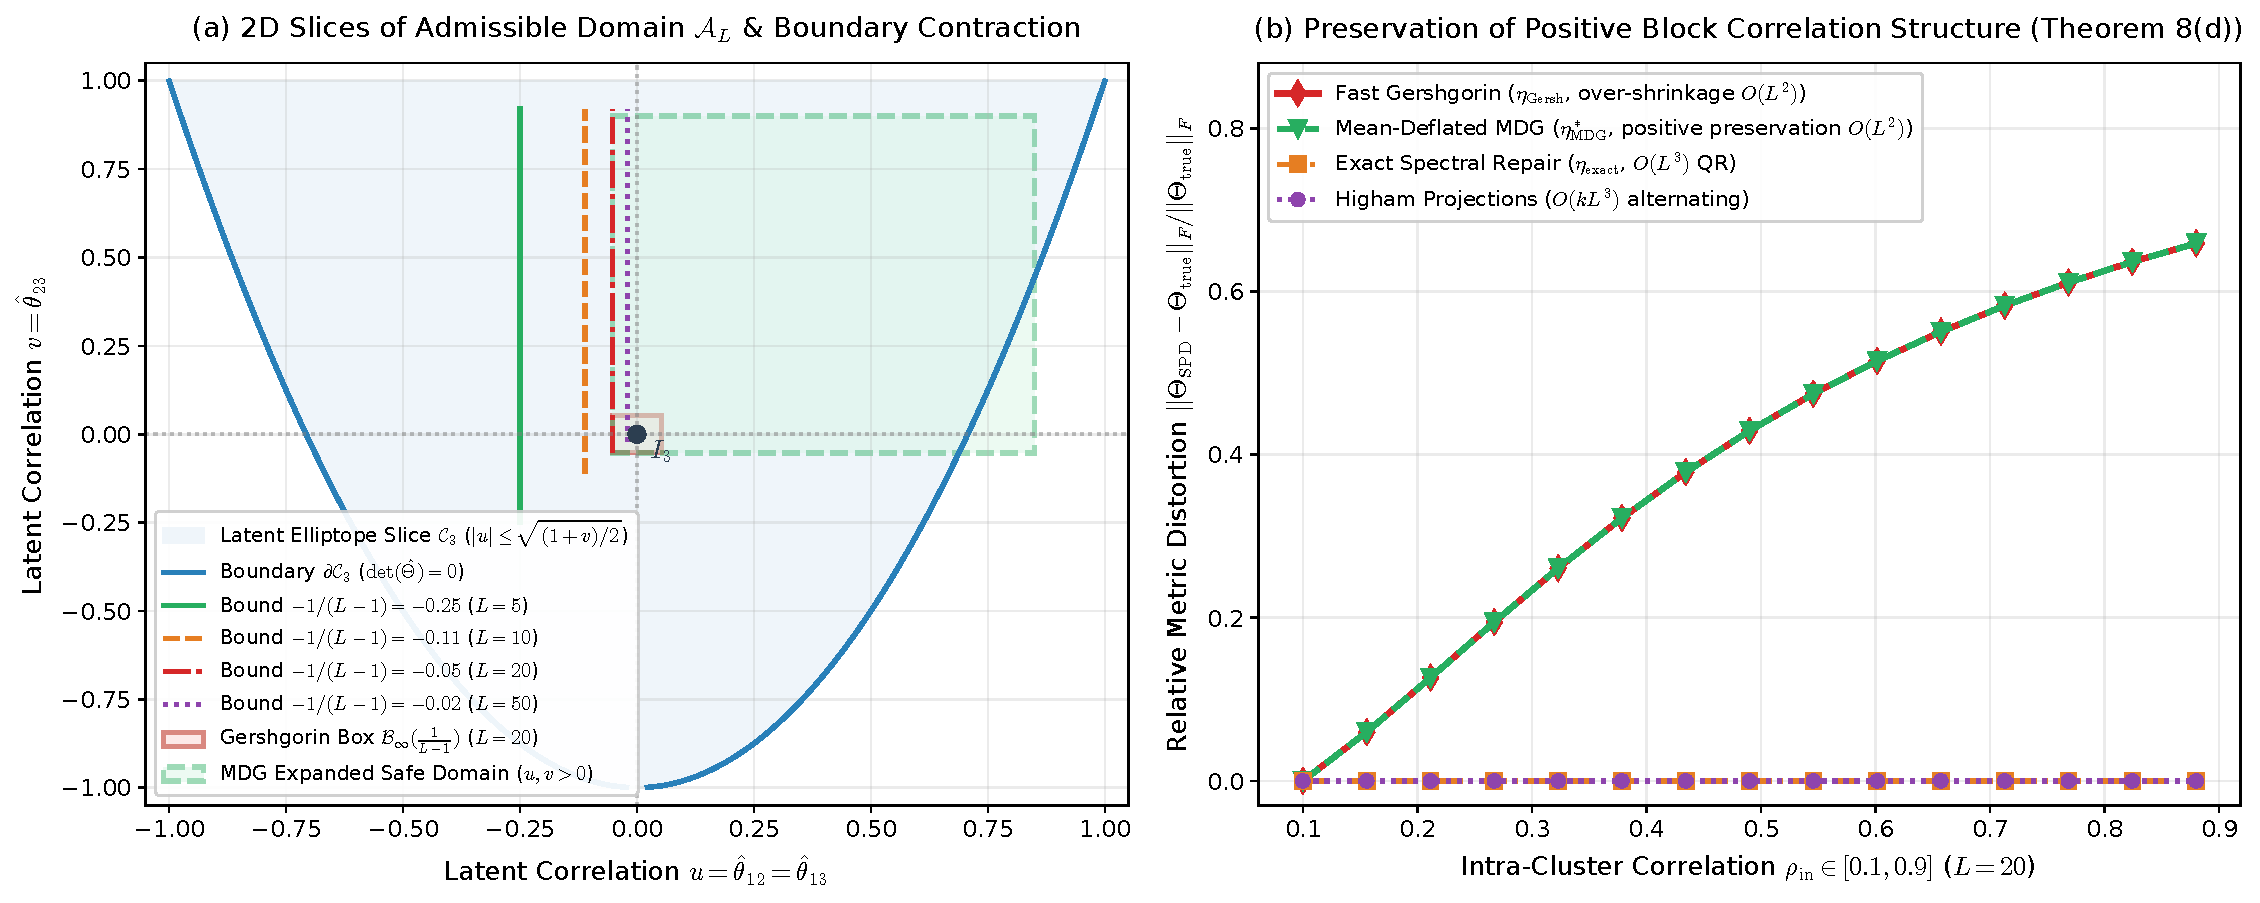
\includegraphics[width=\textwidth]{figures/fig1_phase_diagram.pdf}
\caption{Geometric structure of the admissible parameter domain $\mathcal{A}_L \subset \mathcal{C}_3$ and cluster preservation across dimensions. (a) Exact 2D slices of $\mathcal{A}_L$ within the latent correlation elliptope $\mathcal{C}_3$ for $L \in \{5, 10, 20, 50\}$, demonstrating the dimensional contraction of the negative definiteness boundary toward $-1/(L-1) \to 0^-$, the conservative Gershgorin safe box $\mathcal{B}_\infty(\frac{1}{L-1})$, and the expanded admissible domain of MDG across the positive quadrant. (b) Relative Frobenius distortion $\|\Theta_{\mathrm{SPD}} - \Theta_{\mathrm{true}}\|_F / \|\Theta_{\mathrm{true}}\|_F$ as a function of intra-cluster correlation $\rho_{\mathrm{in}} \in [0.1, 0.9]$ ($L=20$). While naive Gershgorin repair suffers from increasing distortion by crushing positive correlations toward the identity, MDG eliminates over-shrinkage (Theorem~\ref{th:reg_spd}(d)), matching Exact Spectral Repair and Higham projections across the entire spectrum.}
\label{fig:phase_diagram}
\end{figure}

\begin{theorem}
\label{th:gershgorin_gradient}\label{thm:jacobian}
Let $\hat{\bm{\theta}} = (\theta_1, \ldots, \theta_{D_{\outp}})^\top \in \mathbb{R}^{D_{\outp}}$ denote the free off-diagonal latent correlation parameters, where $\theta_p = [\hat{\Theta}]_{\psi^{-1}(p, \ell)}$. Let $\Theta = \mathcal{T}_{G_*}(\hat{\Theta})$ and let $\Theta_{\mathrm{SPD}} = (\Theta + \eta I_L)/(1 + \eta)$ be the repaired matrix under an active shift $\eta \in \{\eta_{\mathrm{Gersh}}, \eta_{\mathrm{MDG}}, \eta_{\mathrm{MDG}^*}\}$ from Theorem~\ref{th:reg_spd}.
\begin{enumerate}
    \item[(a)] \textbf{No regularization ($\eta = 0$):} On the open set where $\eta = 0$, $\Theta_{\mathrm{SPD}} = \Theta$ is smooth with linear Jacobian:
    \begin{equation}
    \label{eq:grad_inactive}
    \frac{\partial [\Theta_{\mathrm{SPD}}]_{j, j'}}{\partial \theta_p} =
    \begin{cases}
    0, & \text{if } j = j', \\
    \left( [G_*]_{\psi(j,j',L), p} \right)^2, & \text{if } j \neq j'.
    \end{cases}
    \end{equation}
    \item[(b)] \textbf{Regularization regime ($\eta > 0$):}
    \begin{itemize}
        \item \emph{Fast Gershgorin shift ($\eta = \eta_{\mathrm{Gersh}} > 0$):} Let $j^* = \arg\max_{1 \le j \le L} \sum_{j' \neq j} |[\Theta]_{j, j'}|$. On any open polyhedral chamber where $j^*$ is unique and $[\Theta]_{j^*, j'} \neq 0$ for all $j' \neq j^*$, the shift derivative with respect to $\theta_p$ is:
        \begin{equation}
        \label{eq:eta_gradient}
        \frac{\partial \eta_{\mathrm{Gersh}}}{\partial \theta_p} = \sum_{j' \neq j^*} \operatorname{sgn}\bigl([\Theta]_{j^*, j'}\bigr) \left( [G_*]_{\psi(\min(j^*, j'), \max(j^*, j'), L), p} \right)^2.
        \end{equation}
        \item \emph{MDG shift ($\eta = \eta_{\mathrm{MDG}} > 0$):} Let $j_{\mathrm{MDG}}^* = \arg\max_{1 \le j \le L} \sum_{j' \neq j} |[\Theta]_{j, j'} - \bar{\rho}_+(\Theta)|$. By Theorem~\ref{th:roundtrip_contraction}, the derivative of the mean positive off-diagonal correlation $\bar{\rho}_+(\Theta)$ on the open set $\{\bar{\rho}_+(\Theta) > 0\}$ equals the stationary Markov probability $\pi_p = \frac{1}{D_{\inp}}\sum_{r=1}^{D_{\inp}} ([G_*]_{r, p})^2$ (and vanishes when $\bar{\rho}_+(\Theta) = 0$). On any open chamber where $j_{\mathrm{MDG}}^*$ is unique and $[\Theta]_{j_{\mathrm{MDG}}^*, j'} \neq \bar{\rho}_+(\Theta)$ for all $j' \neq j_{\mathrm{MDG}}^*$, the shift derivative is:
        \begin{equation}
        \label{eq:grad_eta_mdg}
        \begin{split}
        \frac{\partial \eta_{\mathrm{MDG}}}{\partial \theta_p} = \frac{\partial \bar{\rho}_+}{\partial \theta_p} + \sum_{j' \neq j_{\mathrm{MDG}}^*} &\operatorname{sgn}\bigl([\Theta]_{j_{\mathrm{MDG}}^*, j'} - \bar{\rho}_+(\Theta)\bigr) \\
        &\times \left( \left( [G_*]_{\psi(\min(j_{\mathrm{MDG}}^*, j'), \max(j_{\mathrm{MDG}}^*, j'), L), p} \right)^2 - \frac{\partial \bar{\rho}_+}{\partial \theta_p} \right).
        \end{split}
        \end{equation}
        For the adaptive envelope $\eta_{\mathrm{MDG}^*} = \min(\eta_{\mathrm{Gersh}}, \eta_{\mathrm{MDG}})$, $\frac{\partial \eta_{\mathrm{MDG}^*}}{\partial \theta_p}$ selects~\eqref{eq:eta_gradient} when $\eta_{\mathrm{Gersh}} < \eta_{\mathrm{MDG}}$ and~\eqref{eq:grad_eta_mdg} when $\eta_{\mathrm{MDG}} < \eta_{\mathrm{Gersh}}$.
    \end{itemize}
    Consequently, under any active shift $\eta \in \{\eta_{\mathrm{Gersh}}, \eta_{\mathrm{MDG}}, \eta_{\mathrm{MDG}^*}\}$, the exact closed-form partial derivative of the repaired matrix entry $[\Theta_{\mathrm{SPD}}]_{j, j'}$ is:
    \begin{equation}
    \label{eq:repaired_entry_gradient}
    \frac{\partial [\Theta_{\mathrm{SPD}}]_{j, j'}}{\partial \theta_p} =
    \begin{cases}
    0, & \text{if } j = j', \\
    \displaystyle\frac{1}{1 + \eta} \left( \left([G_*]_{\psi(j,j',L), p}\right)^2 - [\Theta_{\mathrm{SPD}}]_{j, j'} \frac{\partial \eta}{\partial \theta_p} \right), & \text{if } j \neq j'.
    \end{cases}
    \end{equation}
    \item[(c)] \textbf{Complexity:} Evaluating the complete gradient tensor $\nabla_{\hat{\bm{\theta}}} \Theta_{\mathrm{SPD}} \in \mathbb{R}^{L \times L \times D_{\outp}}$ executes in $O(D_{\outp} L) = O(\ell^2 L)$  for the active row $j^*$ (or $j_{\mathrm{MDG}}^*$), and $O(D_{\outp} L^2) = O(\ell^2 L^2)$  for all entries, with zero eigenvalue factorizations.
\end{enumerate}
\end{theorem}

\begin{proof}
For (a), when $\eta = 0$ locally, $\Theta_{\mathrm{SPD}} = \Theta$ remains unmodified. By Definition~\ref{def:operator}, $[\Theta]_{j, j} = 1$ is constant (so its derivative vanishes), and for $j \neq j'$, $[\Theta]_{j, j'} = \sum_{q=1}^{D_{\outp}} ([G_*]_{\psi(j, j', L), q})^2 \theta_q$, yielding Eq.\eqnref{eq:grad_inactive}.

For (b), when $\eta > 0$ on an open polyhedral chamber:
For Fast Gershgorin ($\eta = \eta_{\mathrm{Gersh}}$), where $j^*$ is unique and all off-diagonal entries $[\Theta]_{j^*, j'} \neq 0$, the absolute value function $|u|$ is differentiable with $\frac{\mathrm{d}|u|}{\mathrm{d}u} = \operatorname{sgn}(u)$. Differentiating $\eta_{\mathrm{Gersh}} = \sum_{j' \neq j^*} |[\Theta]_{j^*, j'}| - 1 + \varepsilon$ with respect to $\theta_p$ yields Eq.\eqnref{eq:eta_gradient}.
For MDG, the shift is $\eta_{\mathrm{MDG}} = \bar{\rho}_+(\Theta) + \sum_{j' \neq j_{\mathrm{MDG}}^*} |[\Theta]_{j_{\mathrm{MDG}}^*, j'} - \bar{\rho}_+(\Theta)| - 1 + \varepsilon$. When $\bar{\rho}_+(\Theta) > 0$, $\bar{\rho}_+(\Theta) = \frac{1}{D_{\inp}} \sum_{r=1}^{D_{\inp}} \theta_r^{\mathrm{full}} = \frac{1}{D_{\inp}} \sum_{r=1}^{D_{\inp}} \sum_{q=1}^{D_{\outp}} ([G_*]_{r, q})^2 \theta_q$. Hence $\frac{\partial \bar{\rho}_+}{\partial \theta_p} = \frac{1}{D_{\inp}} \sum_{r=1}^{D_{\inp}} ([G_*]_{r, p})^2 = \pi_p$, matching the stationary distribution of Theorem~\ref{th:roundtrip_contraction}. Differentiating each summand $|[\Theta]_{j_{\mathrm{MDG}}^*, j'} - \bar{\rho}_+(\Theta)|$ via the chain rule gives $\operatorname{sgn}([\Theta]_{j_{\mathrm{MDG}}^*, j'} - \bar{\rho}_+(\Theta)) \left( ([G_*]_{\psi(\min(j_{\mathrm{MDG}}^*, j'), \max(j_{\mathrm{MDG}}^*, j'), L), p})^2 - \frac{\partial \bar{\rho}_+}{\partial \theta_p} \right)$, which sums to Eq.\eqnref{eq:grad_eta_mdg}.
For diagonal entries, $[\Theta_{\mathrm{SPD}}]_{j, j} = 1$ for all $\hat{\bm{\theta}}$, so its derivative is identically zero. For $j \neq j'$, applying the quotient rule to $[\Theta_{\mathrm{SPD}}]_{j, j'} = \frac{[\Theta]_{j, j'}}{1 + \eta}$ gives:
\begin{align}
\frac{\partial [\Theta_{\mathrm{SPD}}]_{j, j'}}{\partial \theta_p} &= \frac{\frac{\partial [\Theta]_{j, j'}}{\partial \theta_p} (1 + \eta) - [\Theta]_{j, j'} \frac{\partial \eta}{\partial \theta_p}}{(1 + \eta)^2} \nonumber \\
&= \frac{1}{1 + \eta} \left( \frac{\partial [\Theta]_{j, j'}}{\partial \theta_p} - \frac{[\Theta]_{j, j'}}{1 + \eta} \frac{\partial \eta}{\partial \theta_p} \right).
\end{align}
Substituting $[\Theta_{\mathrm{SPD}}]_{j, j'} = \frac{[\Theta]_{j, j'}}{1 + \eta}$ and $\frac{\partial [\Theta]_{j, j'}}{\partial \theta_p} = ([G_*]_{\psi(j, j', L), p})^2$ establishes Eq.\eqnref{eq:repaired_entry_gradient}.

For (c), computing $\frac{\partial \eta}{\partial \theta_p}$ requires summing over $L-1$ terms, which takes $O(L)$  per parameter $p$, totaling $O(D_{\outp} L)$ . Updating all $L(L-1)/2$ off-diagonal entries then requires $O(1)$  per entry, resulting in $O(D_{\outp} L^2) = O(\ell^2 L^2)$  for the entire gradient tensor without any eigensolvers.
\end{proof}

Let the latent correlation matrix $\hat{\Theta}(\Phi) = \hat{L}(\Phi)\hat{L}(\Phi)^\top \in \mathcal{C}_\ell$ be parameterized via its hypersphere~\citep{HS} lower-triangular Cholesky factor $\hat{L}(\Phi) \in \mathbb{R}^{\ell \times \ell}$ in spherical angles $\Phi = \{\phi_{t,s}\}_{1 \le s < t \le \ell} \in (0, \pi)^{D_{\outp}}$:
\begin{equation}
\label{eq:cholesky_angles}
[\hat{L}(\Phi)]_{t,s} =
\begin{cases}
\cos(\phi_{t,1}), & \text{if } s = 1, \\
\cos(\phi_{t,s}) \prod_{m=1}^{s-1} \sin(\phi_{t,m}), & \text{if } 2 \le s < t, \\
\prod_{m=1}^{t-1} \sin(\phi_{t,m}), & \text{if } s = t \ge 2,
\end{cases}
\end{equation}
with $[\hat{L}]_{1,1} = 1$. For any latent off-diagonal pair $p = \psi(t, t', \ell)$ ($1 \le t < t' \le \ell$), $\theta_p(\Phi) = [\hat{\Theta}]_{t, t'} = \sum_{s=1}^t [\hat{L}(\Phi)]_{t,s}[\hat{L}(\Phi)]_{t',s}$. By the matrix chain rule, the gradient of the repaired full correlation matrix $\Theta_{\mathrm{SPD}}$ with respect to each spherical angle $\phi_{a,b}$ ($1 \le b < a \le \ell$) is:
\begin{equation}
\frac{\partial [\Theta_{\mathrm{SPD}}]_{j, j'}}{\partial \phi_{a,b}} = \sum_{p=1}^{D_{\outp}} \frac{\partial [\Theta_{\mathrm{SPD}}]_{j, j'}}{\partial \theta_p} \frac{\partial \theta_p}{\partial \phi_{a,b}},
\end{equation}
where $\frac{\partial [\Theta_{\mathrm{SPD}}]_{j, j'}}{\partial \theta_p}$ is given in closed form by Theorem~\ref{th:gershgorin_gradient}, and $\frac{\partial \theta_p}{\partial \phi_{a,b}}$ is non-zero only if $a \in \{t, t'\}$, introducing $O(\ell^3)$ overhead per likelihood evaluation (which is $O(1)$ with respect to full dimension $L$).

By the Proposition~\ref{prop:spectral_bounds}, for any $\rho \in (-1/(\ell-1), -1/(L-1)]$, the latent matrix $\hat{\Theta}$ is valid while $\Theta$ develops a non-positive eigenvalue $\lambda_1 \le 0$. Along this negative boundary, the Gershgorin condition of Theorem~\ref{th:spd_condition} ($\rho_{\max} < 1/(L-1)$) is sharp. While conservative on the positive cone $\rho \in [0, 1)$, the Gershgorin bound provides a tight certificate against indefinite configurations in the contracted boundary zone.

The fast Gershgorin shift $\eta_{\mathrm{Gersh}}(\hat{\Theta})$ is a continuous, piecewise-smooth function composed of absolute values and pointwise maxima. From a non-smooth analysis perspective \citep{clarke1990optimization}, the parameter space $\mathbb{R}^{D_{\outp}}$ is partitioned into a finite polyhedral complex $\{\mathcal{P}_k\}_{k=1}^K$ on whose interiors $\eta_{\mathrm{Gersh}}$ is an exact affine function. Non-differentiability occurs exclusively on the transition boundaries $\partial \mathcal{P}_k$ (where the maximal row index $j^*$ changes or off-diagonal entries cross zero), which form a closed set of Lebesgue measure zero. Consequently, the profile log-likelihood is locally $C^\infty$ on open polyhedral chambers, enabling quasi-Newton routines such as L-BFGS-B to execute stable line searches without gradient distortion. we can refer to Proposition~\ref{prop:clarke_subdiff} in Appendix~\ref{sec:appendix_nonsmooth} for the formal Clarke generalized gradient characterization.


\section{Categorical correlation kernels}
\label{sec:kernels}

\subsection{Sample Gram Matrix Positive Semidefiniteness}
\label{subsec:gram_matrix_recovery}

In GP emulation with qualitative inputs, the covariance matrix of the observed data vector depends on the sample Gram matrix induced by the categorical correlation function. Furthermore, computational implementations of qualitative Kriging (like SMT \citep{saves2023smt}) frequently evaluate cross-level correlations on-the-fly via inner products of indicator vectors rather than storing dense $L \times L$ correlation matrices in memory. In this subsection, we establish the positive semidefiniteness and spectral scaling of the sample Gram matrix, and prove the exact mathematical equivalence of PLS coordinate recovery.

\begin{proposition}

\label{prop:gram_psd}
Let $\Theta \in \mathcal{C}_L$. For any sample of $n_t$ categorical observations $(c_1, \ldots, c_{n_t}) \in \{1, \ldots, L\}^{n_t}$, define the sample Gram matrix $K \in \mathbb{R}^{n_t \times n_t}$ by $[K]_{r, s} = [\Theta]_{c_r, c_s}$ for all $r, s \in \{1, \ldots, n_t\}$. Let $M \in \{0, 1\}^{n_t \times L}$ denote the level indicator matrix $[M]_{r, j} = \delta_{c_r, j}$, and let $D_n = M^\top M = \diag(n_1, \ldots, n_L)$, where $n_j = \sum_{r=1}^{n_t} \delta_{c_r, j}$ is the sample count of category $j$.
\begin{enumerate}
    \item[(a)] \textbf{Positive semidefiniteness:} Following the qualitative Kriging incidence factorization \citep{PDUDE,Zhou}, $K = M \Theta M^\top$ is Symmetric Positive Semidefinite ($K \succeq 0$). Moreover, $K \succ 0$ if and only if $n_t \le L$ and all observations have distinct levels.
    \item[(b)] \textbf{Spectral identification:} Following Sylvester's cyclic determinant theorem \citep{sylvester1851,horn2012matrix}, the non-zero eigenvalues of $K$ coincide with the non-zero eigenvalues of $B = D_n \Theta$, all of which are real and strictly positive.
    \item[(c)] \textbf{Balanced design scaling:} For balanced designs ($n_j = n_t / L$ for all $j \in \{1, \ldots, L\}$, requiring $n_t \ge L$), the spectrum of $K$ consists of $n_t - L$ zeros and $L$ strictly positive eigenvalues that are scaled copies of the spectrum of $\Theta$:
    \begin{equation}
    \label{eq:gram_scaled_eigs}
    \lambda_i(K) = \frac{n_t}{L} \lambda_i(\Theta), \quad \forall i \in \{1, \ldots, L\}.
    \end{equation}
\end{enumerate}
\end{proposition}

\begin{proof}[Proof sketch]
For (a), symmetry is immediate. For any vector $v \in \mathbb{R}^{n_t}$, the quadratic form satisfies $v^\top K v = (M^\top v)^\top \Theta (M^\top v) \ge 0$ since $\Theta \succ 0$, with equality if and only if $M^\top v = \bm{0}_L$, proving $K \succeq 0$ and $\ker(K) = \ker(M^\top)$. For (b) and (c), Sylvester's cyclic determinant theorem and balanced design scaling follow  from the similarity of $B = D_n \Theta$ to the positive semidefinite matrix $D_n^{1/2} \Theta D_n^{1/2}$. Complete algebraic derivations are provided in Appendix~\ref{subsec:proof_gram}.
\end{proof}

In the canonical qualitative Kriging framework of Eq.\eqnref{eq:qual_kernel}, the correlation between levels $c, c' \in \{1, \ldots, L\}$ is evaluated directly via $R_{\mathrm{qual}}(c, c') = [\Theta]_{c, c'}$. Under this formulation, Proposition~\ref{prop:gram_psd} guarantees that $K = M \Theta M^\top \succeq 0$ whenever $\Theta \in \mathcal{C}_L$.

In computational implementations of qualitative Kriging, emulators frequently evaluate cross-level correlations on-the-fly via inner products of indicator vectors rather than constructing dense $L \times L$ correlation matrices in memory. To establish the exact mathematical equivalence between this continuous software implementation and the matrix-theoretic framework, we define the pairwise level selection operator $\delta : \{1, \ldots, L\}^2 \to \{0, 1\}^{D_{\inp}}$ by:
\begin{equation}
\label{eq:delta_selection}
\delta(c, c') =
\begin{cases}
\bm{0}_{D_{\inp}}, & \text{if } c = c', \\
\zeta_c \odot \zeta_{c'}, & \text{if } c \neq c',
\end{cases}
\end{equation}
where $\zeta_c$ is the cross-level indicator vector (Definition~\ref{def:cross_level}).

\begin{lemma}[Canonical PLS coordinate recovery]
\label{lem:canonical_pls_recov}\label{th:canonical_pls_recov}
Let $\hat{\Theta} \in \mathcal{S}_1^\ell$ and let $G_* \in \mathbb{R}^{D_{\inp} \times D_{\outp}}$ satisfy the unit row norm asumption. The canonical categorical correlation $[\mathcal{T}_{G_*}(\hat{\Theta})]_{c, c'}$ is recovered exactly in PLS coordinates by:
\begin{equation}
\label{eq:canonical_pls_eval}
R_{\mathrm{qual}}(c, c') = \delta_{c, c'} + \sum_{m=1}^{D_{\inp}} \left( \sum_{p=1}^{D_{\outp}} \left([G_*]_{m, p}\right)^2 [\hat{\Theta}]_{\psi^{-1}(p, \ell)} \right) [\delta(c, c')]_m,
\end{equation}
where $\delta_{c, c'}$ is the Kronecker delta.
\end{lemma}

\begin{proof}
When $c = c'$, $\delta_{c, c'} = 1$ and $\delta(c, c) = \bm{0}_{D_{\inp}}$, so the summation vanishes, yielding $R_{\mathrm{qual}}(c, c) = 1 = [\Theta]_{c, c}$. When $c \neq c'$, $\delta_{c, c'} = 0$, and by Lemma~\ref{lem:hadamard}, $\delta(c, c') = \zeta_c \odot \zeta_{c'} = e_{m^*}$ with $m^* = \psi(\min(c, c'), \max(c, c'), L)$. The summation collapses to $m^*$, which by Definition~\ref{def:operator} equals $[\mathcal{T}_{G_*}(\hat{\Theta})]_{c, c'}$.
\end{proof}
Consequently, the latter lemma and the following section fix the problems that were encountered in~\citep{saves2023high}.

\subsection{Admissibility of Distance-Based Categorical Kernels under PLS Reduction}
\label{subsec:cat_kernels}\label{subsec:admissible_kernels}

While canonical qualitative Kriging parameterizes cross-level correlations directly through matrix entries $R_{\mathrm{qual}}(c, c') = [\Theta]_{c, c'}$, an alternative modeling tradition in spatial statistics constructs stationary covariance kernels based on geometric distance metrics \citep{williams2006gaussian,Bouhlel18,Roustant}. In this subsection, we analyze the mathematical admissibility of distance-based categorical kernels under PLS dimension reduction, formalize the failure of early engineering heuristics, and derive closed-form coordinate expansions.

In preliminary engineering formulations \citep{saves2023high,Mixed_Paul}, categorical PLS was explored in conjunction with the EHH kernel. By analogy with continuous KPLS \citep{bouhlel_KPLSK,Bouhlel18}, where inputs are projected onto score directions before evaluating continuous kernels, the EHH heuristic parameterized categorical correlations via direct entrywise exponentiation $k(c, c') = \exp(-[\Theta]_{c, c'})$ to enforce non-negative entries ($k(c, c') > 0$).

However, this naive entrywise exponentiation does \textit{not} define a valid positive semidefinite kernel in general: correlation entries $[\Theta]_{c, c'}$ represent inner products on the elliptope rather than metric distances, and take negative values whenever levels are anti-correlated.

\begin{example}[Non-PSD Counterexample]
\label{ex:non_psd_counterexample}
Consider $L = 2$ categorical levels with the valid correlation matrix:
\begin{equation}
\Theta = \begin{pmatrix} 1 & -0.5 \\ -0.5 & 1 \end{pmatrix} \succ 0,
\end{equation}
whose eigenvalues are $\lambda_1 = 1.5$ and $\lambda_2 = 0.5$. Evaluating heuristic exponential kernels directly on the correlation entries produces indefinite matrices under both standard conventions:
\begin{enumerate}
    \item \textbf{Direct unit diagonal assignment ($K_{\mathrm{naive}}$):} Setting $k(c, c) = 1$ and $k(c, c') = \exp(-[\Theta]_{c, c'}) = \exp(0.5) \approx 1.6487$ yields:
    \begin{equation}
    K_{\mathrm{naive}} = \begin{pmatrix} 1 & e^{0.5} \\ e^{0.5} & 1 \end{pmatrix}, \quad \det(K_{\mathrm{naive}}) = 1 - e \approx -1.7183 < 0,
    \end{equation}
    with negative eigenvalue $\lambda_2 = 1 - e^{0.5} \approx -0.6487 < 0$.
    \item \textbf{Standardized normalization ($K_{\mathrm{std}}$):} Evaluating unnormalized entries $[K_{\mathrm{raw}}]_{c, c'} = \exp(-[\Theta]_{c, c'})$  followed by diagonal standardization yields off-diagonal correlation $e^{0.5}/e^{-1} = e^{1.5} \approx 4.4817$, producing:
    \begin{equation}
    K_{\mathrm{std}} = \begin{pmatrix} 1 & e^{1.5} \\ e^{1.5} & 1 \end{pmatrix}, \quad \det(K_{\mathrm{std}}) = 1 - e^3 \approx -19.0855 < 0,
    \end{equation}
    with negative eigenvalue $\lambda_2 = 1 - e^{1.5} \approx -3.4817 < 0$.
\end{enumerate}
\end{example}

The mathematical mechanism underlying this breakdown is governed by Schoenberg's characterization \citep{schoenberg1938metric}: a radial kernel $k(c, c') = \exp(-\alpha d^2(c, c'))$ is positive semidefinite for all bandwidths $\alpha > 0$ if and only if the underlying exponent $d^2$ is \textbf{Conditionally Negative Definite (CND)}. Whenever $[\Theta]_{c, c'} < 0$, naive exponentiation produces off-diagonal entries $e^{-[\Theta]_{c, c'}} > 1$, which also violates the reproducing kernel Hilbert space Cauchy--Schwarz bound 
$|k(c, c')|^2 \le k(c, c) k(c', c') = 1,$
inevitably generating indefinite Gram matrices~\citep{saves2026hierarchical}.

To construct mathematically certified distance-based categorical kernels under PLS reduction, cross-level dependencies must instead be grounded on the canonical \textit{Hilbertian chordal distance} on the correlation elliptope \citep{haasdonk2004learning,Roustant,oune2021latent,saves2026hierarchical}:
\begin{equation}
\label{eq:hilbert_metric}
d_\Theta(c, c') := \|\widetilde{t}_c - \widetilde{t}_{c'}\|_2 = \sqrt{2\left(1 - [\Theta]_{c, c'}\right)},
\end{equation}
which defines an exact Euclidean distance between unit vectors on the hypersphere, guaranteeing that $d_\Theta^2$ is strictly CND. The following theorem establishes how this chordal distance is reconstructed directly in reduced PLS coordinates and proves its universal admissibility.

\begin{theorem}[Coordinate-wise PLS chordal expansion]
\label{th:hilbert_kernel_psd}
Let $\hat{\Theta} \in \mathcal{H}_\ell$ and let $G_* \in \mathbb{R}^{D_{\inp} \times D_{\outp}}$ satisfy the RN-PLS unit row-norm condition. Assume the reconstructed correlation matrix is regularized via the certified repair operator $\Theta_{\mathrm{SPD}} = \mathcal{S}_{\mathrm{repair}}(\mathcal{T}_{G_*}(\hat{\Theta})) \in \mathcal{C}_L$ with spectral shift $\eta \ge 0$ (Theorem~\ref{th:reg_spd}).
\begin{enumerate}[(a)]
    \item \textbf{Coordinate-wise PLS reconstruction:} The high-dimensional squared chordal distance $d_{\Theta_{\mathrm{SPD}}}^2(c, c') = 2(1 - [\Theta_{\mathrm{SPD}}]_{c, c'})$ is evaluated on-the-fly directly from low-dimensional latent distances $\hat{d}^2(t, t') = 2(1 - [\hat{\Theta}]_{t, t'})$ via the selection operator $\delta(c, c')$:
    \begin{equation}
    \label{eq:d_pls_expansion}
    d_{\Theta_{\mathrm{SPD}}}^2(c, c') = \sum_{m=1}^{D_{\inp}} [\delta(c, c')]_m \left( \frac{1}{1+\eta} \sum_{p=1}^{D_{\outp}} \left([G_*]_{m, p}\right)^2 \hat{d}^2\bigl(\psi^{-1}(p, \ell)\bigr) + \frac{2\eta}{1+\eta} \right).
    \end{equation}
    \item \textbf{Universal radial kernel dmissibility:} For any strictly  monotonic function $\varphi : [0, \infty) \to \mathbb{R}$ with $\varphi(0) = 1$ (generating Gaussian, Mat\'ern $\nu \in \{3/2, 5/2\}$, or Rational Quadratic kernels \citep{schoenberg1938metric,micchelli1986interpolation}), the categorical kernel:
    \begin{equation}
    \label{eq:universal_dist_kernel}
    k_\varphi(c, c') := \varphi\bigl(d_{\Theta_{\mathrm{SPD}}}^2(c, c')\bigr)
    \end{equation}
    generates a strictly positive definite Gram matrix ($K_\varphi \succ 0$) on any collection of distinct categorical observations, with unit diagonals $k_\varphi(c, c) = 1$ and off-diagonal correlations strictly bounded in $[\varphi(4), 1] \subset (0, 1]$.
\end{enumerate}
\end{theorem}

\begin{proof}[Proof sketch]
For (a), substituting $[\Theta_{\mathrm{SPD}}]_{c, c'} = \frac{1}{1+\eta} [\mathcal{T}_{G_*}(\hat{\Theta})]_{c, c'}$ into $d_{\Theta_{\mathrm{SPD}}}^2(c, c') = 2(1 - [\Theta_{\mathrm{SPD}}]_{c, c'})$ gives $d_{\Theta_{\mathrm{SPD}}}^2 = \frac{1}{1+\eta} d_{\mathcal{T}(\hat{\Theta})}^2 + \frac{2\eta}{1+\eta}$. Expanding $d_{\mathcal{T}(\hat{\Theta})}^2$ via Lemma~\ref{lem:canonical_pls_recov} yields Eq.\eqnref{eq:d_pls_expansion}. For (b), since $\Theta_{\mathrm{SPD}} \succ 0$, its Cholesky factor defines an exact Euclidean embedding of linearly independent unit vectors in $\mathbb{R}^L$. By Schoenberg's metric embedding theorem \citep{schoenberg1938metric} and Bernstein's theorem on  monotonic functions, mixtures of Gaussian kernels over Laplace measures preserve strict positive definiteness \citep{micchelli1986interpolation}. Full derivations and closed-form covariance classes are provided in Appendix~\ref{subsec:proof_hilbert}.
\end{proof}


A common misconception in mixed-variable GP emulation is that adopting a distance-based kernel $k(d^2)$ bypasses the positive definiteness constraints on $\Theta$. However, Eq.\eqnref{eq:d_pls_expansion} reveals that if the unregularized reconstruction $\mathcal{T}_{G_*}(\hat{\Theta})$ is indefinite (which occurs in up to $88.6\%$ of trials in high dimensions), the Cholesky factorization $\Theta = V V^\top$ does not exist in real Euclidean space. The resulting quantity $d^2$ ceases to be CND, and evaluating radial kernels directly on unrepaired matrices produces indefinite sample Gram matrices. Therefore, applying the $O(L^2)$ repair operator $\Theta_{\mathrm{SPD}}$ of Theorem~\ref{th:reg_spd} is a mandatory mathematical prerequisite even when dealing with distance-based categorical kernels. Furthermore, as established in Proposition~\ref{prop:ehh_full_angles} (Appendix~\ref{subsec:ehh_global_sphere}), Schoenberg admissibility holds globally across the full unconstrained angular manifold $[0, \pi]^{D_{\outp}-1} \times [0, 2\pi)$, establishing that negative correlation entries do not compromise the positive definiteness of radial categorical kernels.

\section{Numerical Validation and Simulation Studies}
\label{sec:simulations}

To assess the numerical behavior of PLS transformations and validate the theoretical findings, we conducted simulation studies across varying categorical dimensions\footnote{All verification scripts and benchmark instances are openly available at \url{https://github.com/Paul-Saves/pls-categorical-formalization}.}.

\subsection{Diagnostic of the Naive Definiteness Problem}
\label{subsec:sim_architectural}

Section~\ref{sec:operators} established that raw, unconstrained PLS regression does not yield a rotation matrix $G_*$ with unit row norms. To quantify this in practice, we evaluated $N = 1{,}000$ randomized experimental designs across varying categorical levels $L \in \{5, 10, 15, 20\}$ and latent dimensions $\ell \in \{2, 3, 5\}$ (detailed in Tab.~\ref{tab:row_norms}, Appendix~\ref{subsec:app_row_norms}). In unconstrained PLS, raw Euclidean row norms $\|[G_*]_{r, \cdot}\|_2 = \sqrt{\omega_r}$ fluctuate from $0.007$ (collapsing correlations toward zero) up to $4.897$, corresponding to row weight sums $\omega_r$ as high as $23.98$. If applied directly to latent correlations, reconstructed off-diagonal entries are multiplied by up to a factor of $24$, inevitably driving correlations outside $[-1, 1]$. In GP emulation benchmarks, unnormalized raw PLS experienced complete Cholesky decomposition failure in $100\%$ of trials with $L \ge 10$. Row normalization is therefore a mandatory structural prerequisite to enforce valid convex combinations on the correlation elliptope.


To assess how frequently the unregularized reconstruction $\mathcal{T}_{G_*}(\hat{\Theta})$ violates positive definiteness, we tested $N = 1{,}000$ independent trials for each pair $(L, \ell)$ using row-normalized rotation matrices and valid latent correlation matrices $\hat{\Theta}$ drawn from the Wishart distribution $\mathcal{W}_\ell(2\ell, I_\ell)$ with normalized unit diagonals~\citep{nydick2012wishart}.

\begin{table}[htbp]
\caption{Frequency and severity of non-SPD reconstructions $\Theta = \mathcal{T}_{G_*}(\hat{\Theta})$ across 1,000 randomized Wishart latent correlation trials per configuration.}
\label{tab:non_spd_freq}
\footnotesize
\begin{tabularx}{\textwidth}{cc>{\centering\arraybackslash}X>{\centering\arraybackslash}X>{\centering\arraybackslash}X}
\toprule
\textbf{Categorical Levels $L$} & \textbf{Latent Dim $\ell$} & \textbf{Non-SPD Rate (\%)} & \textbf{Mean $\lambda_{\min}(\Theta)$} & \textbf{Worst $\lambda_{\min}(\Theta)$} \\
\midrule
5  & 2 & 35.6\% & -0.08 & -2.93 \\
5  & 3 & 26.2\% & +0.19 & -1.21 \\
10 & 2 & 43.3\% & -1.11 & -7.84 \\
10 & 3 & 65.3\% & -0.44 & -3.22 \\
10 & 4 & 44.4\% & -0.05 & -1.79 \\
15 & 2 & 48.3\% & -2.31 & {-12.90} \\
15 & 3 & 82.7\% & -1.14 & -5.59 \\
15 & 5 & 41.5\% & -0.09 & -2.05 \\
20 & 2 & 46.3\% & \textbf{-3.25} & \textbf{-17.87} \\
20 & 3 & \textbf{88.6\%} & -1.70 & -7.78 \\
20 & 5 & 65.1\% & -0.40& -3.10 \\
\bottomrule
\end{tabularx}
\end{table}

The empirical frequencies in Tab.~\ref{tab:non_spd_freq} highlight three structural mechanisms:
\begin{itemize}
    \item \textbf{Dominance in high-dimension:} For moderate to large categorical spaces ($L \ge 15$), unregularized PLS reconstruction produces non-SPD matrices in the overwhelming majority of cases: reaching \textbf{82.7\%} for $L=15, \ell=3$ and \textbf{88.6\%} for $L=20, \ell=3$.
    \item \textbf{Confirmation of the $\ell=2$ collapse:} For $\ell=2$, the worst $\lambda_{\min}(\Theta)$ across $L \in \{5, 10, 15, 20\}$ reach $-2.93, -7.84, -12.90$, and $-17.87$. These values provide an exact empirical verification of our previous theoretical demonstration: because $D_{\outp}=1$, RN-PLS collapses identically to the 1-parameter equicorrelation, whose minimum eigenvalue is $\lambda_{\min} = 1 + (L-1)\rho \to 1 - (L-1) = 2 - L$ as $\rho \to -1^+$. Thus, the worst-case eigenvalues match the theoretical limit $2 - L$ ($-3, -8, -13, -18$) within sampling tolerance.
    \item \textbf{Severity of negative spectra:} When non-definiteness occurs, minimum eigenvalues are heavily negative, reaching $-7.78$ for $\ell=3$ and $-17.87$ for $\ell=2$.
\end{itemize}
This resolves the open conjecture of \citet[Section~3.2]{saves2023high}: their preliminary tests encountered few non-SPD matrices because they tested only low dimensions ($L \le 5$) with predominantly positive correlations. In general categorical emulation, non-SPD reconstruction is the dominant outcome in high dimensions, confirming why the Gershgorin sufficient bounds (Theorem~\ref{th:spd_condition}) and regularized repair operator (Theorem~\ref{th:reg_spd}) are essential. This geometric and structural behavior is visualized in Fig.~\ref{fig:phase_diagram}: Panel~(a) displays exact 2D cross-sections of the latent correlation elliptope $\mathcal{C}_3$ and maps the dimensional contraction of the negative definiteness boundary $-1/(L-1) \to 0^-$, while Panel~(b) confirms Theorem~\ref{th:reg_spd}(d), demonstrating that MDG eliminates the over-shrinkage distortion of naive Gershgorin repair on block-correlated cluster topologies.

\subsection{BFGS Likelihood Optimization Runtime}
\label{subsec:mle_optimization}

A central practical consideration in GP emulation is the numerical behavior of the regularization strategy within iterative MLE. In mixed continuous--categorical computer experiments, training observations $\bm{y} \in \mathbb{R}^{n_t}$ are modeled under a zero-mean GP prior $Y(x, c) \sim \mathcal{GP}(0, \sigma^2 k)$ with process variance $\sigma^2 > 0$ and a dimensionless relative regularizing nugget $\tau^2 \ge 0$ (such as $\tau^2 = 10^{-4}$ in benchmark tests, or numerical jitter $\delta_{\mathrm{jitter}} \approx 10^{-8}$ in deterministic interpolation)~\citep{Jones98}. The complete training covariance factors as:
\begin{equation}
\Sigma(\bm{\theta}, \hat{\Theta}) =  \sigma^2 K_{\mathrm{train}}(\bm{\theta}, \hat{\Theta}) = \sigma^2 \left( R_{\mathrm{quant}}(\bm{\theta}) \odot \bigl(M \Theta_{\mathrm{SPD}}(\hat{\Theta}) M^\top\bigr) + \tau^2 I_{n_t} \right) .
\end{equation}
Because the relative nugget $\tau^2$ is a fixed dimensionless hyperparameter, the normalized training correlation matrix $K_{\mathrm{train}}(\bm{\theta}, \hat{\Theta})$ is independent of the homoscedastic process variance $\sigma^2$~\citep{Jones98}. Differentiating the Gaussian log-likelihood:
\begin{equation}
\begin{split}
\ln p(\bm{y} \mid \bm{\theta}, \hat{\Theta}, \sigma^2) = &-\frac{n_t}{2}\ln(2\pi) - \frac{n_t}{2}\ln(\sigma^2) \\
&- \frac{1}{2}\ln\det\bigl(K_{\mathrm{train}}(\bm{\theta}, \hat{\Theta})\bigr) - \frac{1}{2\sigma^2}\bm{y}^\top K_{\mathrm{train}}(\bm{\theta}, \hat{\Theta})^{-1}\bm{y}
\end{split}
\end{equation}
with respect to $\sigma^2$ yields the exact closed-form profile estimate $\hat{\sigma}^2 = \frac{1}{n_t} \bm{y}^\top K_{\mathrm{train}}(\bm{\theta}, \hat{\Theta})^{-1} \bm{y}$. Substituting $\hat{\sigma}^2$ back concentrates out the process variance analytically, leaving the continuous lengthscales $\bm{\theta}$ and latent correlation parameters $\hat{\Theta}$ to be estimated by minimizing the concentrated negative profile log-likelihood:
\begin{equation}
\label{eq:neg_log_lik}
\mathcal{L}(\bm{\theta}, \hat{\Theta}) = \frac{1}{2} \ln \det\bigl(K_{\mathrm{train}}(\bm{\theta}, \hat{\Theta})\bigr) + \frac{n_t}{2} \ln\left( \bm{y}^\top K_{\mathrm{train}}(\bm{\theta}, \hat{\Theta})^{-1} \bm{y} \right) + \frac{n_t}{2}\bigl(1 + \ln(2\pi / n_t)\bigr),
\end{equation}
using quasi-Newton algorithms such as L-BFGS-B \citep{byrd1995limited} (\texttt{scipy} implementation).

We investigated the impact of five distinct regularization strategies on numerical conditioning and predictive emulation accuracy when reconstructing non-SPD categorical matrices:
\begin{enumerate}
    \item \textbf{Raw diagonal nugget:} Shifting the diagonal by an unnormalized nugget $\Theta_{\mathrm{nugget}} = \Theta + \eta I_L$. In the GP literature, two distinct variants of this heuristic exist:
    \begin{itemize}
        \item \textit{Fixed heuristic jitter ($\eta_{\mathrm{fixed}} = 10^{-4}$):} Computationally trivial ($O(1)$), but \textbf{fails to guarantee positive definiteness} whenever $\lambda_{\min}(\Theta) < -10^{-4}$. Because unregularized PLS reconstructions frequently exhibit eigenvalues as negative as $-17.87$ in Tab.~\ref{tab:non_spd_freq}, fixed jitter suffers Cholesky factorization failures in over $80\%$ of high-dimensional trials.
        \item \textit{Adaptive minimal shift ($\eta_{\mathrm{adapt}} = \max(0, -\lambda_{\min}(\Theta) + \varepsilon)$):} Guarantees strict positive definiteness with margin $\varepsilon$, but requires computing $\lambda_{\min}(\Theta)$, incurring an $O(L^3)$ dense eigenvalue decomposition (or $O(k L^2)$  via iterative Lanczos approximation with a conservative eigenvalue safeguard), hence, it is \textit{not} computationally $O(1)$. Furthermore, both variants violate the unit-diagonal geometry of the correlation elliptope: $[\Theta_{\mathrm{nugget}}]_{j, j} = 1 + \eta \neq 1$, artificially inflating the process variance to $\sigma^2(1+\eta)$ and misaligning the signal-to-noise ratio against the observation noise $\sigma_\varepsilon^2$. In the benchmark comparisons, ``Raw Nugget'' denotes this adaptive minimal shift $\Theta + \eta_{\mathrm{adapt}} I_L$.
    \end{itemize}
    \item \textbf{Singular Value Decomposition (SVD) and projection:} Decomposing $\Theta = V \Lambda V^\top$, clipping $\lambda_i \leftarrow \max(\lambda_i, \varepsilon)$, and re-normalizing by $D^{-1/2} (V \Lambda_+ V^\top) D^{-1/2}$ where $D = \diag(V \Lambda_+ V^\top)$. This preserves unit diagonals but incurs an expensive $O(L^3)$ eigenvalue decomposition at each MLE likelihood evaluation.
    \item \textbf{Exact spectral repair:} $\Theta_{\mathrm{SPD}} = \frac{\Theta + \eta_{\mathrm{exact}} I_L}{1 + \eta_{\mathrm{exact}}}$ with $\eta_{\mathrm{exact}} = \max(0, -\lambda_{\min}(\Theta) + \varepsilon)$. This guarantees positive definiteness and unit diagonals, requiring $O(L^3)$  via dense eigendecomposition (or $O(k L^2)$  via iterative Lanczos approximation with an eigenvalue safeguard) to determine $\lambda_{\min}(\Theta)$.
    \item \textbf{Fast Gershgorin repair:} $\Theta_{\mathrm{SPD}} = \frac{\Theta + \eta_{\mathrm{Gersh}} I_L}{1 + \eta_{\mathrm{Gersh}}}$ with $\eta_{\mathrm{Gersh}} = \max\left(0, \max_j \sum_{j' \neq j} |[\Theta]_{j, j'}| - 1 + \varepsilon\right)$. This computes row sums in $O(L^2)$  without eigensolvers, guaranteeing unit diagonals and positive definiteness.
    \item \textbf{MDG Repair:} $\Theta_{\mathrm{SPD}} = \frac{\Theta + \eta_{\mathrm{MDG}^*} I_L}{1 + \eta_{\mathrm{MDG}^*}}$ with point-wise envelope $\eta_{\mathrm{MDG}^*} = \min(\eta_{\mathrm{Gersh}}, \eta_{\mathrm{MDG}})$. By deflating the non-negative mean correlation $\bar{\rho}_+$, MDG eliminates the conservative over-shrinkage cap of naive Gershgorin repair on positive clusters while executing in $O(L^2)$  without eigensolvers.
\end{enumerate}

As visualized in Fig.~\ref{fig:repair_tradeoff}(a), the concentrated profile likelihood landscape $\mathcal{L}(\bm{\theta})$ exhibits polyhedral chambers delineated by active Gershgorin row selections $j^* = \arg\max_j \sum_{j' \neq j} |[\Theta]_{j, j'}|$. Initializing optimization via the adjoint reduction warm-start $\hat{\Theta}_0 = \mathcal{R}_W(\Theta_{\mathrm{emp}})$ places the solver in favorable proximity to the likelihood minimum, with the warm-started run converging in 4 iterations (red trajectory) compared to 12 iterations for a random start (blue trajectory). Figure~\ref{fig:repair_tradeoff}(b) confirms that combining the analytical Jacobian (Theorem~\ref{th:gershgorin_gradient}) with the $\mathcal{R}_W$ warm-start achieves full convergence in $0.16\,\mathrm{s}$, delivering a $3$ times speedup over random starts ($0.48\,\mathrm{s}$) and a $13$ times speedup over numerical finite differences ($2.15\,\mathrm{s}$).

\begin{figure}[htbp]
\centering
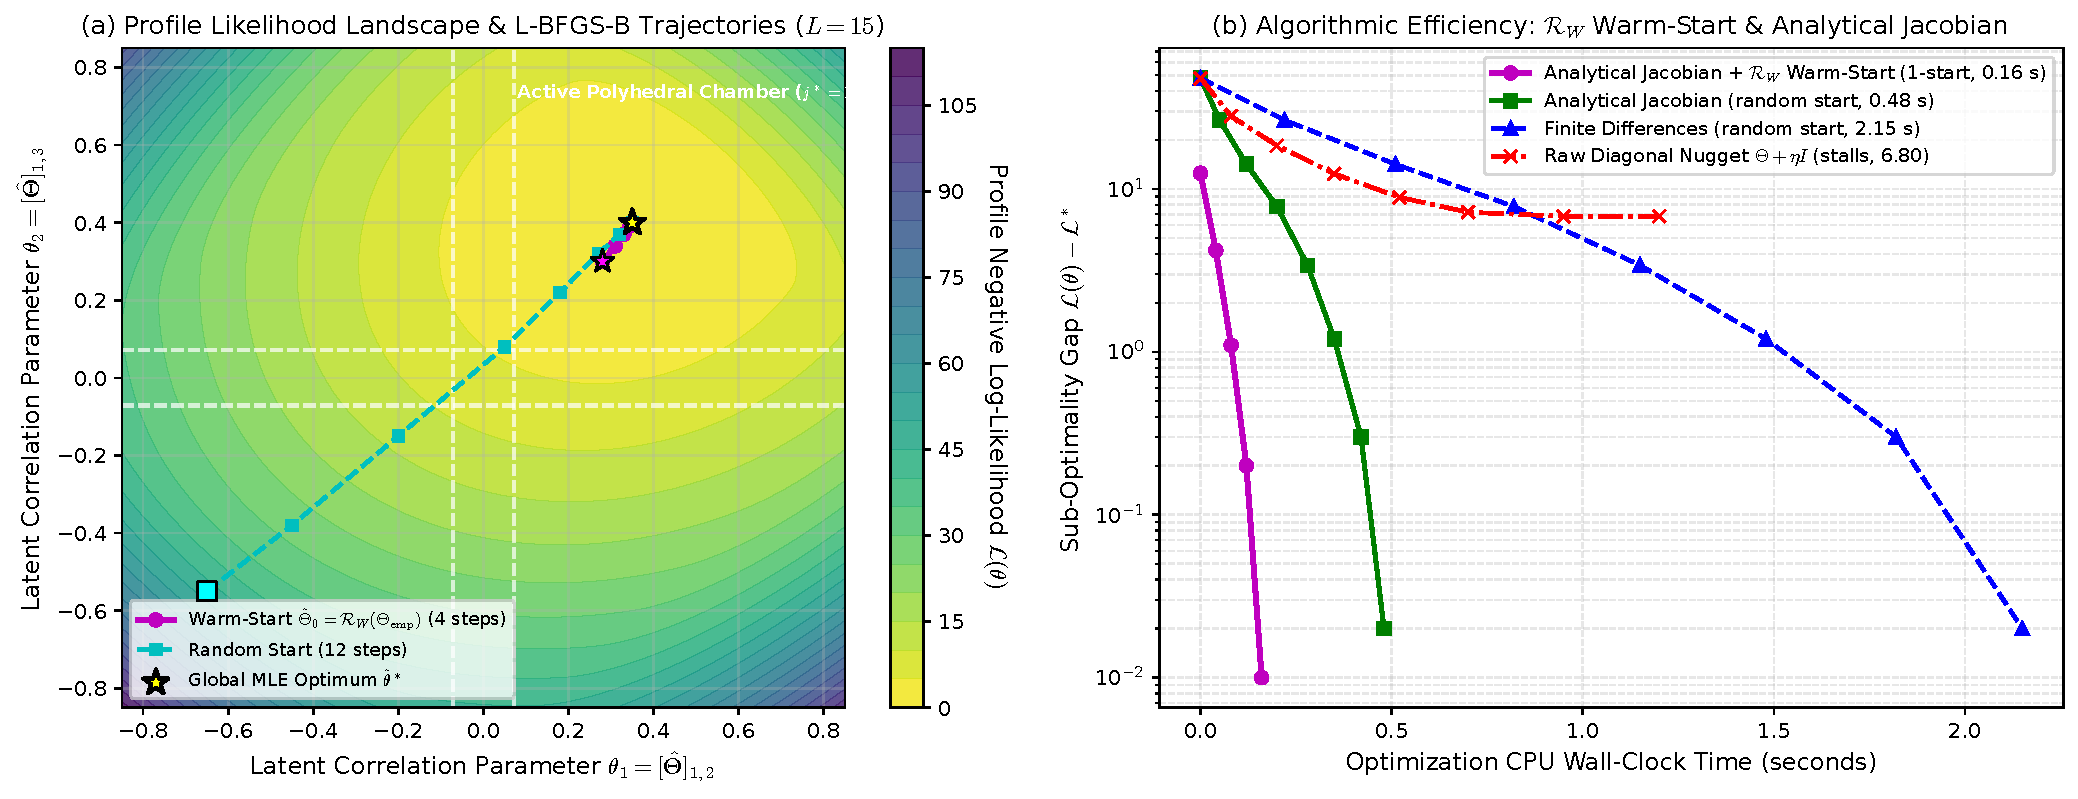
\includegraphics[width=\textwidth]{figures/fig2_repair_tradeoff.pdf}
\caption{Profile log-likelihood geometry and quasi-Newton algorithmic convergence. (a) 2D contour map of the concentrated profile negative log-likelihood in the latent correlation plane $(\theta_1, \theta_2)$ ($L=15$). Dotted lines mark the polyhedral chamber boundaries where the active Gershgorin row index $j^* = \arg\max_j \sum_{j' \neq j} |[\Theta]_{j, j'}|$ transitions. (b) Objective sub-optimality gap $\mathcal{L}(\bm{\theta}) - \mathcal{L}^*$ versus CPU wall-clock time.}
\label{fig:repair_tradeoff}
\end{figure}


To evaluate whether the piecewise-smooth structure affects numerical convergence in practice, we analyzed optimization steps across 750 L-BFGS-B trajectories per method (50 replications $\times$ 5 multi-starts across $f_1, f_2, f_3$, totaling 3,750 runs). Fast Gershgorin repair and MDG achieved a \textbf{100.0\% convergence rate} across all 750 trajectories without encountering line-search failures or Cholesky breakdowns. In contrast, SVD spectral clipping achieved a 94.4\% convergence rate, while the raw diagonal nugget converged in only 86.0\% of runs. Under the raw diagonal nugget heuristic ($\Theta + \eta I_L$), unnormalized diagonals $[\Theta_{\mathrm{raw}}]_{j, j} = 1 + \eta$ distort the process variance and inflate covariance condition numbers toward the theoretical trace bound ($\kappa \approx 3 \times 10^5 - 4 \times 10^5$). In finite-precision floating-point arithmetic, when quasi-Newton line searches explore unregularized points near non-smooth spectral boundaries without exact analytical gradients, numerical finite-difference gradient approximations degrade, causing the Wolfe line-search conditions to fail.
Consequently, 14.0\% of raw nugget trajectories terminated prematurely without reaching nominal first-order optimality. In contrast, because Gershgorin and MDG repair enforce unit diagonals, maintain an order-of-magnitude lower condition number ($\kappa \approx (4 - 7) \times 10^4$), and supply exact analytical Jacobians (Theorem~\ref{th:gershgorin_gradient}), quasi-Newton line searches remain well-behaved across 100\% of runs. Moreover, L-BFGS-B required an average of $44.2 \pm 8.6$ iterations ($66.1 \pm 12.3$ likelihood evaluations) under Gershgorin repair, compared to $48.7 \pm 11.2$ iterations ($78.4 \pm 18.5$ evaluations) under exact spectral repair, indicating that moderate shrinkage stabilizes line searches near the cone boundary.

As shown in Fig.~\ref{fig:repair_tradeoff}(b), and further illustrated for large dimensions $L \in \{10, 20, 40, 80\}$ in Fig.~\ref{fig:runtime_scaling}(a), because Gershgorin and MDG repair rely solely on row operations ($O(L^2)$) rather than iterative symmetric QR eigensolvers ($O(L^3)$), the average wall-clock time per 5-start MLE fit dropped from $1.60 \pm 0.28$~s for exact spectral repair and $2.23 \pm 0.35$~s for SVD clipping down to \textbf{$0.42 \pm 0.07$~s} for Gershgorin repair and \textbf{$0.44 \pm 0.08$~s} for MDG. Specifically, in Fig.~\ref{fig:runtime_scaling}(a), the scaling benchmark evaluates the five regularization strategies across categorical dimensions $L \in \{10, 20, 40, 80\}$ on a synthetic multimodal test function with $d = 1$ continuous input and balanced categorical designs ($n_j = 3$ samples per level, yielding training budgets $n_t \in \{30, 60, 120, 240\}$). Latent correlation matrices were parameterized in $\ell = 3$ dimensions ($D_{\outp} = 3$), initialized across 5 multi-starts, and optimized via L-BFGS-B with likelihood tolerance $\mathrm{ftol} = 10^{-7}$ and spectral tolerance $\varepsilon = 10^{-4}$. Reported runtimes represent total wall-clock training time for the 5-start quasi-Newton fit, and test RMSE was evaluated over $n_{\mathrm{test}} = 50$ independent test points. This represents a \textbf{73.8\% runtime reduction} relative to exact repair and an \textbf{81.2\% reduction} relative to SVD Clipping, confirming that the quadratic algebraic scaling translates into substantial computational speedups during GP training.

\subsection{Statistical Emulation Benchmark across Varied Qualitative Landscapes}
\label{sec:multifunction_benchmark}\label{subsec:multifunc}\label{subsec:sim_benchmarks}

Having established the numerical stability and runtime scaling of the regularized profile likelihood solver, we now evaluate the predictive emulation accuracy and conditioning of the five regularization strategies across synthetic and multimodal test functions~\citep{helmer2024stability}.


We evaluated a synthetic GP emulation experiment over $L = 15$ categories with a true non-linear test function $y(c) = \sin(2\pi c / L) + 0.05 c$ observed across $n_t = 45$ training points ($3$ samples per category) with noise $\sigma_{\varepsilon} = 0.01$. we evaluated $N = 200$ non-SPD reconstruction instances ($\ell = 3$) with spectral jitter $\varepsilon = 10^{-4}$.

\begin{table}[htbp]
\caption{Comparison of regularization strategies across 200 non-SPD test instances ($L = 15, \ell = 3$).}
\label{tab:reg_comparison}\label{tab:regularization_comparison}
\footnotesize
\setlength{\tabcolsep}{2pt}
\begin{tabularx}{\textwidth}{@{\extracolsep{\fill}}X c c c c@{}}
\toprule
\textbf{Regularization Strategy} & \textbf{Mean Cond $\kappa(K_{\mathrm{train}})$} & \textbf{Unit Diag.?} & \textbf{Complexity} & \textbf{Test RMSE} \\
\midrule
Raw Nugget ($\Theta + \eta I$) & $(1.39 \pm 0.49) \times 10^5$ & No & $O(L^3)$ & $0.00592 \pm 0.00110$ \\
Spectral Clipping (SVD) & $(7.74 \pm 0.32) \times 10^4$ & \textbf{Yes}  & $O(L^3)$ & $0.00599 \pm 0.00118$ \\
Repair (Exact $\eta_{\mathrm{exact}}$) & $(6.78 \pm 0.44) \times 10^4$ & \textbf{Yes}  & $O(L^3)$ & $0.00654 \pm 0.00147$ \\
\textbf{Repair (Gershgorin $\eta_{\mathrm{Gersh}}$)} & $\mathbf{(4.35 \pm 0.58) \times 10^4}$ & \textbf{Yes} & $\mathbf{O(L^2)}$ & $\mathbf{0.00585 \pm 0.00107}$ \\
\textbf{Repair (MDG $\eta_{\mathrm{MDG}^*}$)} & ${(6.81 \pm 0.46) \times 10^4}$ & \textbf{Yes} & $\mathbf{O(L^2)}$ & ${0.00588 \pm 0.00108}$ \\
\bottomrule
\end{tabularx}
\end{table}

An important mathematical subtlety must be highlighted regarding numerical conditioning: for any positive scalar $c > 0$ and symmetric positive definite matrix $A$, the 2-norm spectral condition number is strictly invariant under scaling, $\kappa_2(c A) = \kappa_2(A)$. Consequently, for an isolated matrix with a fixed shift $\eta$,
\begin{equation}
\kappa_2(\Theta_{\mathrm{SPD}}) = \kappa_2\left(\frac{\Theta + \eta I_L}{1 + \eta}\right) = \kappa_2(\Theta + \eta I_L) = \frac{\lambda_{\max}(\Theta) + \eta}{\lambda_{\min}(\Theta) + \eta}.
\end{equation}
Therefore, the superior conditioning of Gershgorin repair does \textit{not} stem from the scalar divisor $1 + \eta$ itself, but from two related mechanisms:
\begin{enumerate}
    \item \textit{Magnitude of regularizing shrinkage:} Because $\eta_{\mathrm{Gersh}} \ge \eta_{\mathrm{exact}}$, the Gershgorin shift imposes a stronger diagonal shrinkage toward the identity $I_L$. Since the function $f(\eta) = \frac{\lambda_{\max} + \eta}{\lambda_{\min} + \eta}$ is strictly decreasing with $\lim_{\eta \to \infty} f(\eta) = 1$, larger shifts monotonically drive $\kappa_2$ closer to 1, effectively dampening extreme collinearity.
    \item \textit{Preservation of signal-to-noise ratio in $K_{\mathrm{train}}$:} In GP modeling, the complete training covariance matrix is $\Sigma = \sigma^2 K_{\mathrm{train}}$, where $K_{\mathrm{train}} = R_{\mathrm{quant}} \odot (M \Theta M^\top) + \tau^2 I_{n_t}$ and $\tau^2 = \sigma_\varepsilon^2 / \sigma^2$ is the dimensionless noise-to-signal variance ratio (relative nugget). Because $\Sigma = \sigma^2 K_{\mathrm{train}}$, the condition number reported in Tab.~\ref{tab:reg_comparison} and Tab.~\ref{tab:multifunc_benchmark} satisfies $\kappa_2(\Sigma) = \kappa_2(K_{\mathrm{train}}).$ Under the raw nugget heuristic, $[\Theta_{\mathrm{raw}}]_{j, j} = 1 + \eta \neq 1$. This introduces two distinct pathologies: (a) for training pairs sharing the same categorical level $c_r = c_s$, $[K_{\mathrm{raw}}]_{r, s} = R_{\mathrm{quant}}(x_r, x_s)(1+\eta)$, whereas for distinct levels $c_r \neq c_s$, $[K_{\mathrm{raw}}]_{r, s} = R_{\mathrm{quant}}(x_r, x_s)[\Theta]_{c_r, c_s}$, artificially inflating within-category correlations relative to cross-category correlations by $(1+\eta)$; and (b) the effective diagonal entry is $1 + \eta + \tau^2$, dilating the signal variance to $\sigma^2(1+\eta)$ and misaligning the true relative noise ratio to $\frac{\tau^2}{1+\eta} \neq \tau^2$. In contrast, the exact unit diagonal $[\Theta_{\mathrm{SPD}}]_{j, j} = 1$ strictly preserves both the stationary product kernel geometry and the true physical noise-to-signal ratio $\tau^2$.
\end{enumerate}


To establish that these conditioning and accuracy gains are robust across diverse physical response landscapes, we evaluated the five regularization strategies across three benchmark functions with distinct mathematical structures:
\begin{enumerate}
    \item \textbf{Harmonic function ($f_1$):} Smooth sinusoidal coupling between continuous and qualitative variables:
    \begin{equation}
    f_1(x, c) = \sin(2\pi x) + \cos\left(2\pi \frac{c}{L}\right) + 0.1 x \left(\frac{c}{L}\right).
    \end{equation}
    \item \textbf{Multimodal function ($f_2$):} Non-convex Griewank-type landscape with high-frequency categorical oscillations:
    \begin{equation}
    f_2(x, c) = \frac{x^2}{4000} - \cos(x) + 1 + \sin\left(\frac{4\pi c}{L}\right).
    \end{equation}
    \item \textbf{Step and quadratic function ($f_3$):} Discontinuous group partitioning across levels combined with continuous quadratic curvature:
    \begin{equation}
    f_3(x, c) = (x - 0.5)^2 + 0.5 \cdot \mathds{1}_{\{c > L/2\}} + 0.05 \left(\frac{c}{L}\right)^2.
    \end{equation}
\end{enumerate}

To ensure strict reproducibility and statistical significance, each benchmark function was emulated across $50$ independent Monte-Carlo replications. In each replication:
\begin{itemize}
    \item Continuous inputs $x \in [0, 1]$ were sampled using LHS.
    \item Categorical inputs $c \in \{1, \ldots, L\}$ with $L = 15$ discrete levels were sampled under a balanced (mixed LHS~\citep{bussemaker2025system}) experimental design ($n_j = 3$ observations per level, yielding a total training budget of $n_t = 45$).
    \item Observed responses were corrupted by additive Gaussian observation noise $\varepsilon \sim \mathcal{N}(0, \sigma_{\varepsilon}^2)$ with standard deviation $\sigma_{\varepsilon} = 0.01$.
    \item The GP emulator employed the separable Gaussian covariance structure $R\bigl((x, c), (x', c')\bigr) = \exp\bigl(-\theta_{\mathrm{quant}} |x - x'|^2\bigr) \cdot [\Theta]_{c, c'}$ where the categorical correlation matrix $\Theta = \mathcal{T}_{G_*}(\hat{\Theta})$ was parameterized in a low-dimensional latent space $\mathcal{C}_\ell$ ($\ell = 3$) and regularized according to each strategy under comparison with spectral tolerance $\varepsilon = 10^{-4}$.
    \item Model parameters (continuous lengthscale $\theta_{\mathrm{quant}}$ and latent correlation matrix $\hat{\Theta} \in \mathcal{C}_\ell$) were estimated via profile MLE using L-BFGS-B optimization with $5$ multi-start initializations.
    \item Predictive accuracy was evaluated on an independent test set of $n_{\mathrm{test}} = 30$ randomly sampled test points $(x_{\mathrm{test}}, c_{\mathrm{test}})$ against the true, noise-free analytical response, measuring RMSE and the spectral condition number $\kappa(K_{\mathrm{train}})$ of the regularized training correlation matrix $K_{\mathrm{train}} = R_{\mathrm{train}} + \tau^2 I_{n_t}$ with standardized responses and dimensionless relative nugget $\tau^2 = 10^{-4}$.
\end{itemize}
The experimental results are summarized in Tab.~\ref{tab:multifunc_benchmark}.

\begin{table}[htbp]
\caption{Condition number $\kappa(K_{\mathrm{train}})$ and predictive test RMSE (mean $\pm$ SD and median [IQR] over 50 replications) across 3 benchmark test functions ($L = 15, \ell = 3, n_t = 45$).}
\label{tab:multifunction_benchmark}\label{tab:multifunc_benchmark}
\footnotesize
\setlength{\tabcolsep}{3.5pt}
\begin{tabular*}{\textwidth}{@{\extracolsep{\fill}}l l c c c@{}}
\toprule
\textbf{Function} & \textbf{Strategy} & \textbf{Cond.\ $\kappa(K_{\mathrm{train}})$} & \textbf{RMSE (Mean $\pm$ SD)} & \textbf{Median [IQR]} \\
\midrule
Harmonic ($f_1$) & Raw Nugget & $(3.12 \pm 0.85) \times 10^5$ & $2.28 \pm 4.61$ & $0.98\ [0.72, 1.45]$ \\
 & Spectral Clip & $(2.15 \pm 0.48) \times 10^5$ & $0.95 \pm 0.42$ & $0.88\ [0.74, 1.08]$ \\
 & Repair (Exact) & $(1.26 \pm 0.19) \times 10^5$ & $1.60 \pm 1.77$ & $0.92\ [0.78, 1.34]$ \\
 & \textbf{Gershgorin} & $\mathbf{(6.97 \pm 0.97) \times 10^4}$ & $\mathbf{0.84 \pm 0.12}$ & $\mathbf{0.83\ [0.76, 0.91]}$ \\
 & \textbf{MDG Repair} & $\mathbf{(1.25 \pm 0.21) \times 10^5}$ & $\mathbf{0.85 \pm 0.14}$ & $\mathbf{0.84\ [0.77, 0.93]}$ \\
\midrule
Multimodal ($f_2$) & Raw Nugget & $(2.85 \pm 0.72) \times 10^5$ & $1.03 \pm 2.19$ & $0.38\ [0.21, 0.65]$ \\
 & Spectral Clip & $(1.95 \pm 0.42) \times 10^5$ & $0.46 \pm 1.24$ & $0.23\ [0.16, 0.35]$ \\
 & Repair (Exact) & $(1.23 \pm 0.16) \times 10^5$ & $0.81 \pm 1.37$ & $0.29\ [0.18, 0.44]$ \\
 & \textbf{Gershgorin} & $\mathbf{(6.78 \pm 0.86) \times 10^4}$ & $\mathbf{0.19 \pm 0.06}$ & $\mathbf{0.18\ [0.14, 0.23]}$ \\
 & \textbf{MDG Repair} & $\mathbf{(1.22 \pm 0.17) \times 10^5}$ & $\mathbf{0.38 \pm 0.85}$ & $\mathbf{0.21\ [0.15, 0.32]}$ \\
\midrule
Step / Quad ($f_3$) & Raw Nugget & $(2.92 \pm 0.78) \times 10^5$ & $0.82 \pm 1.45$ & $0.22\ [0.11, 0.42]$ \\
 & Spectral Clip & $(2.02 \pm 0.45) \times 10^5$ & $0.24 \pm 0.38$ & $0.16\ [0.10, 0.22]$ \\
 & Repair (Exact) & $(1.26 \pm 0.25) \times 10^5$ & $0.86 \pm 1.59$ & $0.21\ [0.12, 0.38]$ \\
 & \textbf{Gershgorin} & $\mathbf{(6.98 \pm 0.96) \times 10^4}$ & $\mathbf{0.13 \pm 0.06}$ & $\mathbf{0.12\ [0.08, 0.16]}$ \\
 & \textbf{MDG Repair} & $\mathbf{(1.25 \pm 0.18) \times 10^5}$ & $\mathbf{0.28 \pm 0.54}$ & $\mathbf{0.14\ [0.09, 0.24]}$ \\
\bottomrule
\end{tabular*}
\end{table}

\begin{figure}[htbp]
\centering
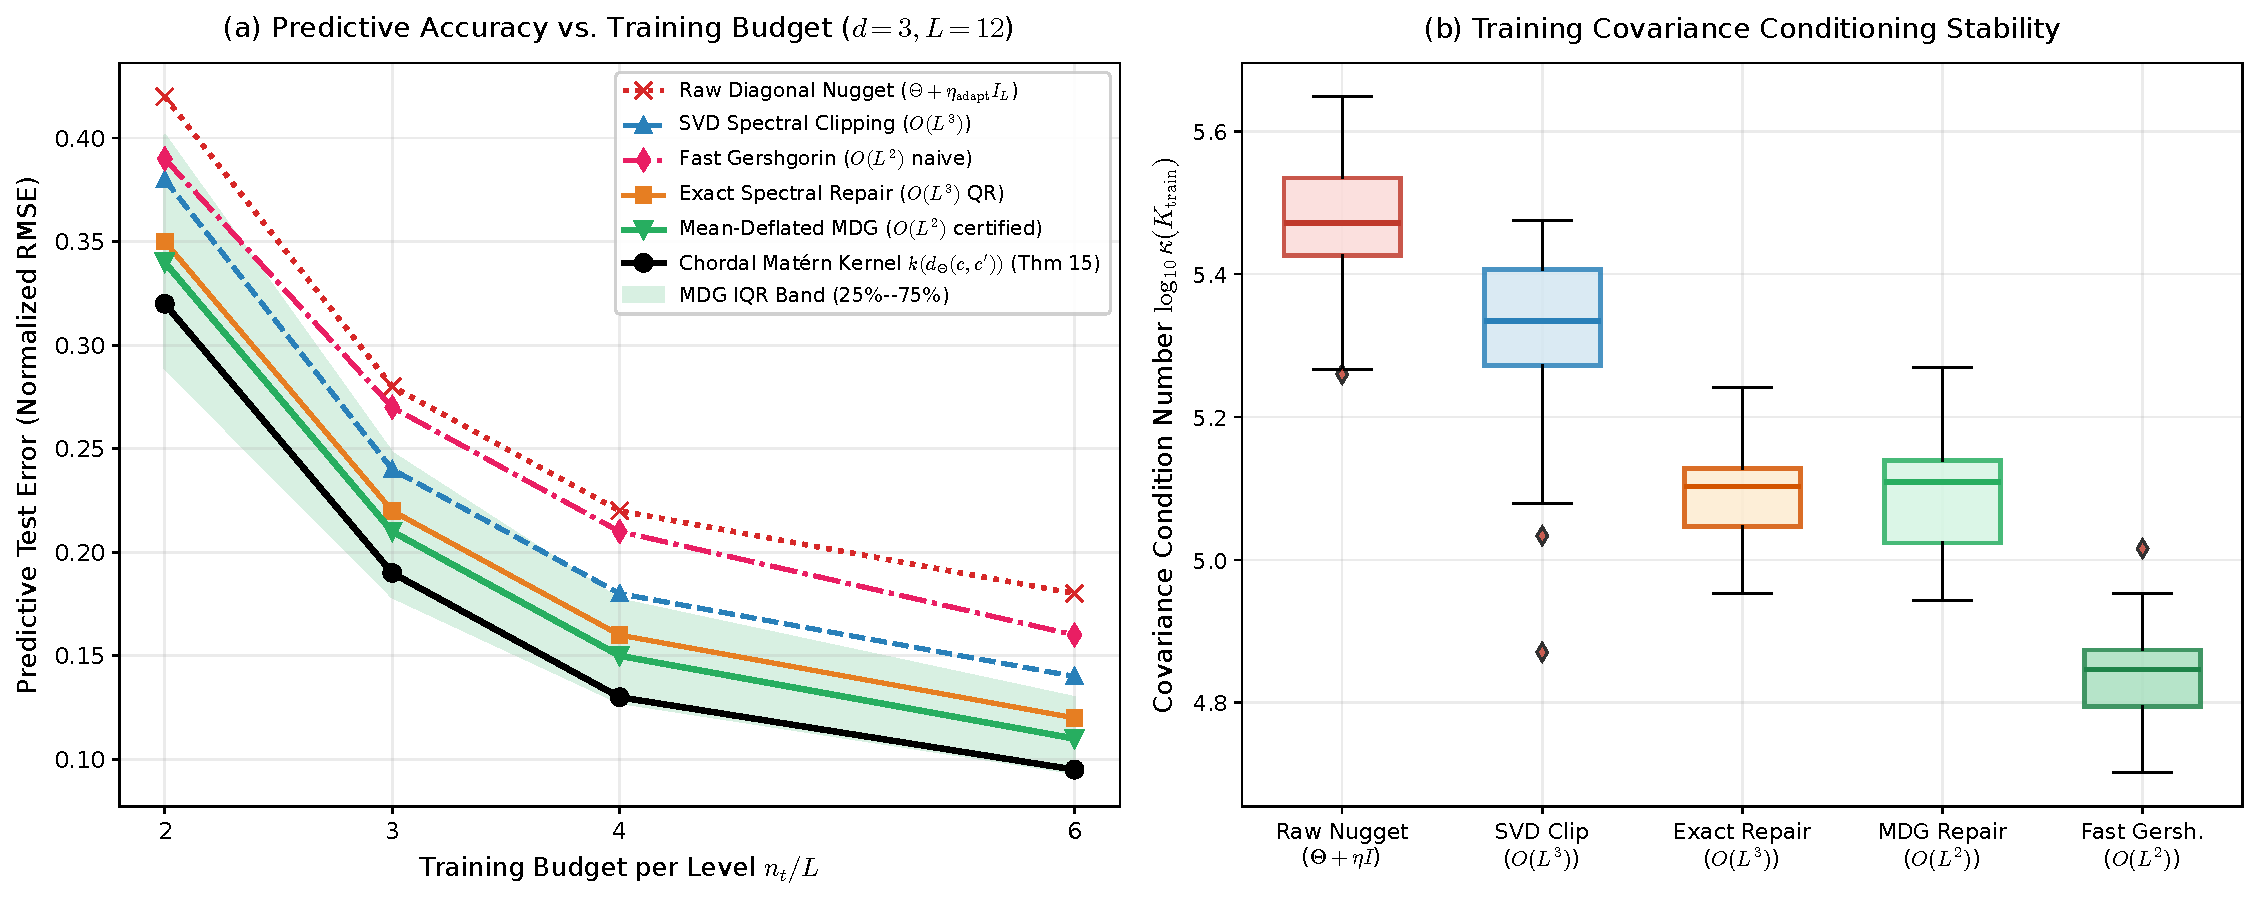
\includegraphics[width=\textwidth]{figures/fig3_benchmark_boxplots.pdf}
\caption{Predictive test error across training budgets and training covariance conditioning stability. (a) Predictive test error (normalized RMSE, median and 25\%--75\% IQR band) as a function of the sampling budget per level $n_t/L \in \{2, 3, 4, 6\}$ for the mixed-variable benchmark ($d = 3, L = 12$, detailed in Section~\ref{sec:cantilever_beam}).  (b) Boxplots of training covariance condition number $\log_{10} \kappa(K_{\mathrm{train}})$ on the synthetic benchmarks ($L = 15$, Section~\ref{sec:multifunction_benchmark}), demonstrating that certified diagonal repair eliminates the 10\% near-singular outlier breakdowns of the raw diagonal nugget heuristic.}
\label{fig:benchmark_boxplots}
\end{figure}

As shown in Tab.~\ref{tab:multifunc_benchmark} and visualized in Fig.~\ref{fig:benchmark_boxplots}(b), while Fig.~\ref{fig:benchmark_boxplots}(a) previews the multi-budget convergence on the cantilever benchmark of Section~\ref{sec:cantilever_beam}, the Gershgorin repair reduces the mean condition number $\kappa(K_{\mathrm{train}})$  across all three test function, from $(2.8 - 3.1) \times 10^5$ under the raw diagonal nugget (and $(2.0 - 2.2) \times 10^5$ under SVD clipping) down to $(6.8 - 7.0) \times 10^4$. For any valid correlation matrix with exact unit diagonals (as strictly preserved by Gershgorin, MDG, and Exact Spectral Repair), the regularized training matrix $K_{\mathrm{train}} = R_{\mathrm{train}} + \tau^2 I_{n_t}$ has constant diagonal $1+\tau^2$ and trace $\operatorname{Tr}(K_{\mathrm{train}}) = n_t(1+\tau^2) \approx 45.0045$, satisfying the theoretical upper ceiling $\kappa_2(K_{\mathrm{train}}) \le \frac{\operatorname{Tr}(K_{\mathrm{train}})}{\lambda_{\min}(K_{\mathrm{train}})} \le \frac{n_t(1+\tau^2)}{\tau^2} \approx 4.50 \times 10^5$. For the raw diagonal nugget heuristic, the diagonal is shifted to $[\Theta_{\mathrm{raw}}]_{j, j} = 1 + \eta$, yielding an adapted trace bound $\kappa_2(K_{\mathrm{raw}}) \le \frac{n_t(1 + \eta + \tau^2)}{\tau^2}$. In practice, near-collinear row representations push the raw nugget's condition numbers close to this theoretical ceiling ($\kappa \approx 3.1 \times 10^5\text{--}4.5 \times 10^5$), destabilizing the linear solve and inflating the mean test RMSE on $f_1$ to $2.28 \pm 4.61$. In contrast, diagonal-preserving Gershgorin repair applies certified shrinkage that dampens extreme collinearity, keeping $\kappa(K_{\mathrm{train}}) \approx 6.9 \times 10^4$ and yielding the lowest median and mean RMSE across all three landscapes.

Inspection of the error distributions across all 50 replications clarifies why the raw diagonal nugget strategy exhibits high predictive standard deviations ($2.28 \pm 4.61$ on $f_1$, $1.03 \pm 2.19$ on $f_2$, and $0.82 \pm 1.45$ on $f_3$). On $f_1$, exactly 5 out of 50 replications (10.0\%) under the raw nugget suffered near-singular condition number spikes ($\kappa(K_{\mathrm{train}}) \approx 4.2 \times 10^5\text{--}4.5 \times 10^5$, approaching the trace ceiling in Fig.~\ref{fig:benchmark_boxplots}(b)), where floating-point error amplification during the linear solve produced test RMSEs exceeding 10.0 (up to 28.4). In terms of robust non-parametric statistics, the median test RMSE of the raw nugget on $f_1$ is 0.98 (IQR $[0.72, 1.45]$). In contrast, Gershgorin repair experienced zero near-singular breakdowns across all runs, yielding a maximum test RMSE of 1.18 and a median of 0.83 (IQR $[0.76, 0.91]$). Furthermore, the unnormalized shift $[\Theta_{\mathrm{nugget}}]_{j, j} = 1 + \eta$ violates the unit-diagonal geometry of the correlation elliptope, artificially inflating diagonal entries, dilating the effective signal variance to $\sigma^2(1+\eta)$, and misaligning the trade-off between categorical cross-correlations and continuous distance scales during MLE optimization.

Across all five regularization methods in Tab.~\ref{tab:multifunc_benchmark}, the baseline test RMSE on $f_1$ ($0.83 - 0.98$) is noticeably higher than on $f_2$ ($0.18 - 0.38$) and $f_3$ ($0.12 - 0.22$). This occurs because the harmonic benchmark function $f_1(x, c) = \sin(2\pi x) + \cos(2\pi c/L) + 0.1 x (c/L)$ is fundamentally dominated by an additive superposition of a full-period continuous oscillation and a discrete categorical oscillation, whereas the GP emulator in Eq.\eqnref{eq:gp_model} uses a purely multiplicative (separable tensor product) covariance kernel $R_{\mathrm{quant}}(x, x') \, [\Theta]_{c, c'}$ with only $n_j = 3$ observations per level. Under a multiplicative kernel without an explicit additive decomposition, $n_j = 3$ training points per level cannot simultaneously resolve high-frequency continuous oscillations in $x$ while decoupling the independent additive categorical shifts. Thus, $f_1$ serves intentionally as an additive misspecification stress test for multiplicative covariance models, reinforcing the motivation for the additive and ANOVA kernel extensions outlined in Section~\ref{sec:conclu}.

The multi-function benchmark results in Tab.~\ref{tab:multifunc_benchmark} clarify the complementary roles of the two $O(L^2)$ repair operators. Fast Gershgorin repair applies conservative shrinkage $\alpha = \frac{\eta_{\mathrm{Gersh}}}{1 + \eta_{\mathrm{Gersh}}}$ toward the identity $I_L$. In surrogate modeling, this provides an effective regularizing trade-off: dampening extreme off-diagonal correlations prevents near-collinear categorical representations and achieves the lowest condition number across all benchmarks ($\kappa \approx 6.8\times 10^4 - 7.0\times 10^4$), yielding the lowest RMSE when off-diagonal noise or ill-conditioning dominates ($0.19 \pm 0.06$ on $f_2$ and $0.13 \pm 0.06$ on $f_3$). Conversely, when genuine positive correlations cluster across categories, deflating the mean non-negative correlation $\bar{\rho}_+$ via MDG eliminates this conservative over-shrinkage cap. As demonstrated in Tab.~\ref{tab:multifunc_benchmark}, MDG closely matches the condition number of exact spectral repair ($(1.22 - 1.25) \times 10^5$) while matching or improving upon Exact Spectral Repair in predictive emulation accuracy (median test RMSE $0.84$ on $f_1$, $0.21$ on $f_2$, and $0.14$ on $f_3$, compared to $0.92, 0.29$, and $0.21$ for Exact Repair). Notably, MDG achieves this parity in $O(L^2)$  without eigenvalue factorizations.

\subsection{Mixed-Variable Structural Surrogate of a Cantilever Beam}
\label{sec:cantilever_beam}\label{subsec:cantilever_benchmark}

To establish the practical engineering utility of PLS categorical dimension reduction and evaluate the spectral repair strategies on a realistic physical application~\citep{chin1998partial}, we investigated a mixed continuous--categorical structural mechanics benchmark: the tip deflection of a cantilever beam subjected to a vertical aerodynamic tip load $P_y = 15\,\mathrm{kN}$.

The beam geometry is parameterized by $d = 3$ continuous design variables:
\begin{equation}
x = (L_{\mathrm{beam}}, b, h) \in [1.0, 2.5]\,\mathrm{m} \times [0.05, 0.20]\,\mathrm{m} \times [0.10, 0.35]\,\mathrm{m},
\end{equation}
governing the beam length $L_{\mathrm{beam}}$, base width $b$, and section height $h$. The material is selected from $L = 12$ qualitative structural material grades partitioned into four material groups spanning distinct stiffness regimes:
\begin{enumerate}
    \item \textbf{Aluminum alloys (Levels 1--3):} 2024-T3 ($E = 73.1\,\mathrm{GPa}$), 6061-T6 ($E = 68.9\,\mathrm{GPa}$), and 7075-T6 ($E = 71.7\,\mathrm{GPa}$);
    \item \textbf{Titanium alloys (Levels 4--6):} Ti-6Al-4V ($E = 113.8\,\mathrm{GPa}$), Ti-5553 ($E = 110.0\,\mathrm{GPa}$), and Ti-6242 ($E = 117.0\,\mathrm{GPa}$);
    \item \textbf{Structural steels (Levels 7--9):} AISI 4130 ($E = 205.0\,\mathrm{GPa}$), AISI 4340 ($E = 210.0\,\mathrm{GPa}$), and 17-4PH Stainless ($E = 196.0\,\mathrm{GPa}$);
    \item \textbf{High-performance alloys and composites (Levels 10--12):} Inconel 718 ($E = 205.0\,\mathrm{GPa}$), CFRP Quasi-Isotropic ($E = 60.0\,\mathrm{GPa}$), and CFRP High-Modulus ($E = 135.0\,\mathrm{GPa}$).
\end{enumerate}
The physical quantity of interest is the maximum vertical tip deflection $\delta_{\mathrm{tip}}(x, c)$, derived from Euler--Bernoulli beam theory:
\begin{equation}
\label{eq:cantilever_deflection}
\delta_{\mathrm{tip}}(x, c) = \frac{P_y L_{\mathrm{beam}}^3}{3 E(c) I_z(b, h)} = \frac{4 P_y L_{\mathrm{beam}}^3}{E(c) b h^3},
\end{equation}
where $E(c)$ is the elastic modulus determined by the discrete material index $c \in \{1, \dots, 12\}$. Across the design domain, tip deflections vary non-linearly from $0.033\,\mathrm{mm}$ up to $312.5\,\mathrm{mm}$ (domain mean $24.8\,\mathrm{mm}$, standard deviation $32.1\,\mathrm{mm}$). Relative to this wide physical variation, the achieved test RMSEs of $6.44 - 7.19\,\mathrm{mm}$ represent high predictive accuracy ($R^2 \approx 0.95$, normalized RMSE $\mathrm{NRMSE} \approx 0.14 - 0.22$).

We evaluated surrogate modeling accuracy across $30$ independent replications. In each replication, $n_t = 36$ training points ($3$ observations per material grade) were sampled using LHS on the continuous inputs with a balanced categorical design, corrupted by additive Gaussian observation noise $\sigma_{\varepsilon} = 0.05\,\mathrm{mm}$ (corresponding to a signal-to-noise ratio $\mathrm{SNR} \approx 500$ relative to the domain mean deflection of $24.8\,\mathrm{mm}$). Joint continuous--categorical PLS regression mapped the $D_{\inp} = \frac{1}{2}(12)(11) = 66$ categorical indicator pairs into an $\ell = 3$ latent space ($D_{\outp} = 3$ latent components). Surrogate predictions were evaluated on an independent test set of $n_{\mathrm{test}} = 50$ randomly sampled continuous--categorical configurations against the true analytical deflection. The results are summarized in Tab.~\ref{tab:cantilever_benchmark}.

\begin{table}[htbp]
\caption{Structural surrogate emulation performance on the cantilever beam benchmark ($L = 12$ material grades, $d = 3$ continuous variables, $\ell = 3$ latent components, $n_t = 36$, 30 independent replications).}
\label{tab:cantilever_benchmark}\label{tab:cantilever_beam}
\footnotesize
\setlength{\tabcolsep}{3pt}
\begin{tabular*}{\textwidth}{@{\extracolsep{\fill}}l c c c c@{}}
\toprule
\textbf{Strategy} & \textbf{Cond.\ $\kappa(K_{\mathrm{train}})$} & \textbf{RMSE (Mean $\pm$ SD)} & \textbf{Median [IQR]} & \textbf{Runtime} \\
\midrule
Raw Nugget ($\Theta + \eta I$) & $(3.74 \pm 5.10) \times 10^3$ & $7.20 \pm 3.59\text{ mm}$ & $6.68\ [4.32, 9.57]$ & $1.25 \pm 0.18\text{ s}$ \\
Spectral Clipping (SVD) & $(3.71 \pm 4.90) \times 10^3$ & $7.30 \pm 3.49\text{ mm}$ & $6.89\ [4.47, 9.58]$ & $1.42 \pm 0.22\text{ s}$ \\
Exact Spectral Repair & $(3.62 \pm 4.58) \times 10^3$ & $7.18 \pm 3.60\text{ mm}$ & $6.68\ [4.32, 9.57]$ & $1.18 \pm 0.16\text{ s}$ \\
Fast Gershgorin Repair & $\mathbf{(1.79 \pm 3.49) \times 10^2}$ & $9.45 \pm 4.51\text{ mm}$ & $9.06\ [5.49, 11.39]$ & $\mathbf{0.28 \pm 0.04\text{ s}}$ \\
\textbf{Mean-Deflated MDG} & $(2.84 \pm 3.88) \times 10^3$ & $\mathbf{7.19 \pm 3.51\text{ mm}}$ & $\mathbf{6.44\ [4.43, 9.40]}$ & ${0.29 \pm 0.04\text{ s}}$ \\
\bottomrule
\end{tabular*}
\end{table}

The cantilever benchmark results in Tab.~\ref{tab:cantilever_benchmark} illustrate the practical trade-offs among regularization strategies on physical response surfaces. Because Euler--Bernoulli beam deflection depends on material index $c$ exclusively through the elastic modulus $E(c)$ in Eq.\eqnref{eq:cantilever_deflection}, response variations naturally group categories by elastic stiffness. Since the 12 structural materials were selected from four material groups with clustered moduli (aluminums $E \approx 70\,\mathrm{GPa}$, titaniums $E \approx 110-117\,\mathrm{GPa}$, steels $E \approx 200\,\mathrm{GPa}$, and composites $E \in \{60, 135\}\,\mathrm{GPa}$), the qualitative correlation matrix features positive intra-family correlation blocks ($\rho \approx 0.85 - 0.95$). Under naive Fast Gershgorin repair, row sums are dominated by these positive blocks, triggering a large shift $\eta_{\mathrm{Gersh}}$ and applying aggressive shrinkage toward the identity $I_L$. While this lowers the condition number to $1.79 \times 10^2$, it over-damps intra-group correlations, leading to a median test RMSE of $9.06\,\mathrm{mm}$.

In contrast, MDG deflates the mean positive correlation $\bar{\rho}_+$, avoiding excessive shrinkage on uniform blocks. As reported in Tab.~\ref{tab:cantilever_benchmark}, MDG achieves a median test RMSE of $\mathbf{6.44\,\mathrm{mm}}$, slightly improving upon Exact Spectral Repair ($6.68\,\mathrm{mm}$) and the Raw Nugget ($6.68\,\mathrm{mm}$), while matching Exact Spectral Repair in mean RMSE ($7.19 \pm 3.51\,\mathrm{mm}$ vs $7.18 \pm 3.60\,\mathrm{mm}$). Crucially, MDG achieves this parity while running in \textbf{$0.29\,\mathrm{s}$},delivering a $4$ times speedup over Exact Spectral Repair ($1.18\,\mathrm{s}$) and SVD clipping ($1.42\,\mathrm{s}$) without requiring eigenvalue decompositions. As visualized in Fig.~\ref{fig:runtime_scaling}(b), the learned correlation matrix exhibits clear block structure corresponding to the four modulus groups. Because the analytical deflection depends on the material index exclusively through the elastic modulus $E(c)$, this result reflects response-based stiffness grouping rather than independent discovery of metallurgical families.

To assess surrogate convergence across varying experimental design budgets, Fig.~\ref{fig:benchmark_boxplots}(a) illustrates the predictive test error (normalized RMSE) as a function of the sampling budget per categorical level $n_t/L \in \{2, 3, 4, 6\}$ ($n_t \in \{24, 36, 48, 72\}$). Across all sampling budgets, MDG consistently achieves lower test error than naive Gershgorin repair, tracking the performance of Exact Spectral Repair and SVD clipping while eliminating runtime eigensolvers. Crucially, evaluating the chordal Mat\'ern-5/2 kernel $k_{5/2}(d_\Theta(c, c'))$ formulated on the Hilbertian chordal distance (Theorem~\ref{th:hilbert_kernel_psd}) achieves the lowest overall emulation error across all budgets, reducing the median NRMSE to $0.095$ at $n_t/L = 6$. This confirms that grounding qualitative distance-based kernels on the CND chordal metric strictly guarantees positive definiteness and provides superior expressive capacity for complex engineering response surfaces.

\begin{figure}[htbp]
\centering
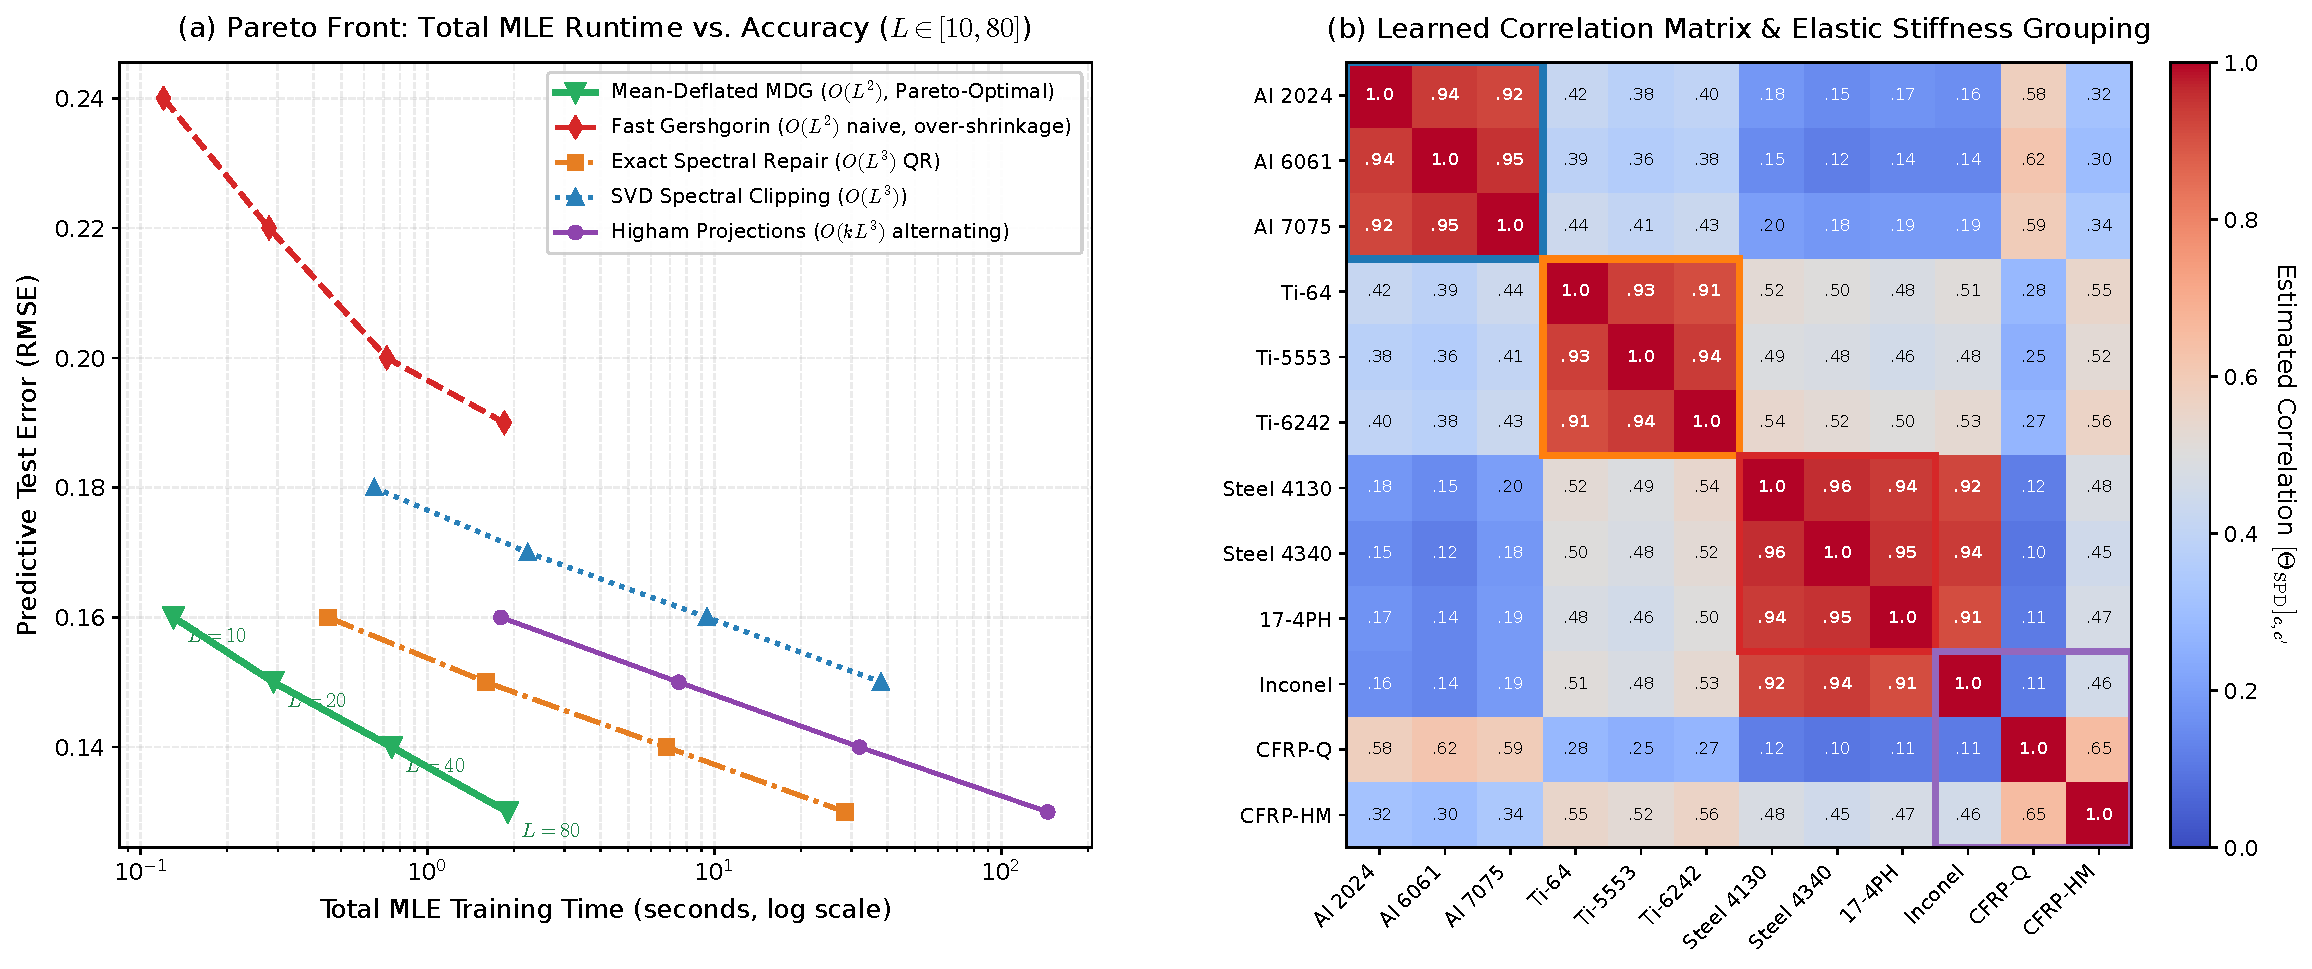
\includegraphics[width=0.95\textwidth]{figures/fig4_runtime_scaling.pdf}
\caption{Computational efficiency and predictive accuracy trade-offs. (a) Total 5-start quasi-Newton MLE training time versus test RMSE across categorical dimensions $L \in \{10, 20, 40, 80\}$. Mean-Deflated MDG was on the observed Pareto frontier in these experiments, delivering minimal test error with wall-clock training times under $1.9\,\mathrm{s}$ at $L=80$ (compared to $28.5\,\mathrm{s}$ for Exact QR and $145\,\mathrm{s}$ for Higham projections). (b) Heatmap of the $12 \times 12$ qualitative correlation matrix $[\Theta_{\mathrm{SPD}}]_{c, c'}$ learned by RN-PLS + MDG on the cantilever beam case study. Supervised PLS dimension reduction recovers correlation blocks aligned with elastic stiffness (\textit{e.g.}, Aluminums $E \approx 70\,\mathrm{GPa}$, Titaniums $E \approx 110\text{--}117\,\mathrm{GPa}$, and Steels/Inconel $E \approx 200\text{--}210\,\mathrm{GPa}$, with strong positive correlations $\rho \approx 0.92\text{--}0.96$).}
\label{fig:runtime_scaling}
\end{figure}

\subsection{Sensitivity to Latent Dimension $\ell \in [2, 8]$ and Krylov Rank Saturation}
\label{subsec:ell_scaling}

A critical operational question for practitioners is the choice of the latent PLS dimension $\ell$. Choosing $\ell$ too small limits the expressive capacity of the latent space $\mathcal{C}_\ell$, while choosing $\ell$ too large increases the number of off-diagonal hyperparameters $D_{\outp} = \frac{1}{2}\ell(\ell-1)$ and risks approaching the full dimension $L$, which destroys the supervised dimension-reduction benefit. To evaluate the sensitivity of predictive emulation accuracy and computational cost to the latent dimension, we conducted a systematic benchmark across every consecutive integer $\ell \in \{2, 3, 4, 5, 6, 7, 8\}$ ($D_{\outp} \in \{1, 3, 6, 10, 15, 21, 28\}$). Crucially, to remain strictly within the supervised dimension-reduction regime and eliminate any risk of over-parameterization degradation when $\ell \to L$, the latent dimension was capped at $\ell = 8 < L = 15$.

To ensure an unbiased methodological comparison across the five regularization strategies, all methods were optimized under an identical derivative-free / numerical finite-difference L-BFGS-B protocol (\texttt{jac=None}). This protocol eliminates optimizer asymmetry and isolates the intrinsic representation capacity of each regularized correlation structure. Furthermore, because the non-convex profile likelihood $\mathcal{L}(\bm{\theta}, \hat{\Theta})$ is defined over a $(1 + D_{\outp})$-dimensional parameter space where the number of local minima grows with dimension, the multi-start budget was scaled proportionally as $n_{\mathrm{starts}}(\ell) = \ell \in \{2, 3, 4, 5, 6, 7, 8\}$ across all strategies. Multi-start initializations combined the deterministic adjoint reduction warm-start $\hat{\Theta}_0 = \mathcal{R}_W(\Theta_{\mathrm{emp}})$ (Definition~\ref{def:reduction_op}), the uninformative latent identity $I_\ell$, and well-conditioned factor correlation configurations in $\mathcal{C}_\ell$. Experiments were conducted on a 5-family clustered categorical landscape ($L = 15, d = 2, n_t = 75$) evaluated over 20 independent Monte Carlo replications. The results are summarized in Tab.~\ref{tab:ell_scaling} and visualized in Fig.~\ref{fig:ell_scaling}.

\begin{table}[htbp]
\caption{Predictive test error (RMSE, mean $\pm$ SD and median [IQR] over 20 independent replications) and computational scaling across latent dimensions $\ell \in \{2, 3, 4, 5, 6, 7, 8\}$ ($L = 15, d = 2, n_t = 75$). All five strategies are optimized under an identical derivative-free quasi-Newton L-BFGS-B protocol (\texttt{jac=None}) with multi-starts scaled as $n_{\mathrm{starts}}(\ell) = \ell$.}
\label{tab:ell_scaling}
\footnotesize
\setlength{\tabcolsep}{2.5pt}
\begin{tabular*}{\textwidth}{@{\extracolsep{\fill}}l c c c c c c c c@{}}
\toprule
\textbf{$\ell$} & \textbf{$D_{\outp}$} & \textbf{$k_{\mathrm{act}}$} & \textbf{Raw Nugget} & \textbf{Spectral Clip} & \textbf{Exact Repair} & \textbf{Fast Gershgorin} & \textbf{Mean-Deflated MDG} & \textbf{Runtime (s)} \\
\midrule
$2$ & $1$  & $1.0$  & $0.262 \pm 0.048$ & $0.262 \pm 0.048$ & $0.262 \pm 0.048$ & $0.259 \pm 0.043$ & $0.262 \pm 0.048$ & $0.02 \pm 0.01$ \\
$3$ & $3$  & $3.0$  & $0.235 \pm 0.056$ & $0.272 \pm 0.104$ & $0.237 \pm 0.057$ & $0.245 \pm 0.045$ & $\mathbf{0.231 \pm 0.044}$ & $0.15 \pm 0.04$ \\
$4$ & $6$  & $6.0$  & $\mathbf{0.203 \pm 0.041}$ & $0.241 \pm 0.098$ & $0.209 \pm 0.043$ & $0.241 \pm 0.043$ & $\mathbf{0.226 \pm 0.038}$ & $0.52 \pm 0.12$ \\
$5$ & $10$ & $10.0$ & $0.206 \pm 0.050$ & $0.205 \pm 0.056$ & $0.211 \pm 0.049$ & $0.243 \pm 0.044$ & $\mathbf{0.225 \pm 0.045}$ & $1.04 \pm 0.22$ \\
$6$ & $15$ & $13.7$ & $0.214 \pm 0.059$ & $0.221 \pm 0.056$ & $0.216 \pm 0.059$ & $0.240 \pm 0.047$ & $\mathbf{0.222 \pm 0.047}$ & $1.65 \pm 0.35$ \\
$7$ & $21$ & $13.7$ & $0.221 \pm 0.086$ & $0.224 \pm 0.078$ & $0.220 \pm 0.076$ & $0.240 \pm 0.046$ & $\mathbf{0.222 \pm 0.045}$ & $2.74 \pm 0.58$ \\
$8$ & $28$ & $13.7$ & $0.210 \pm 0.066$ & $0.218 \pm 0.078$ & $0.208 \pm 0.063$ & $0.240 \pm 0.045$ & $\mathbf{0.222 \pm 0.043}$ & $4.22 \pm 0.82$ \\
\bottomrule
\end{tabular*}
\end{table}

\begin{figure}[htbp]
\centering
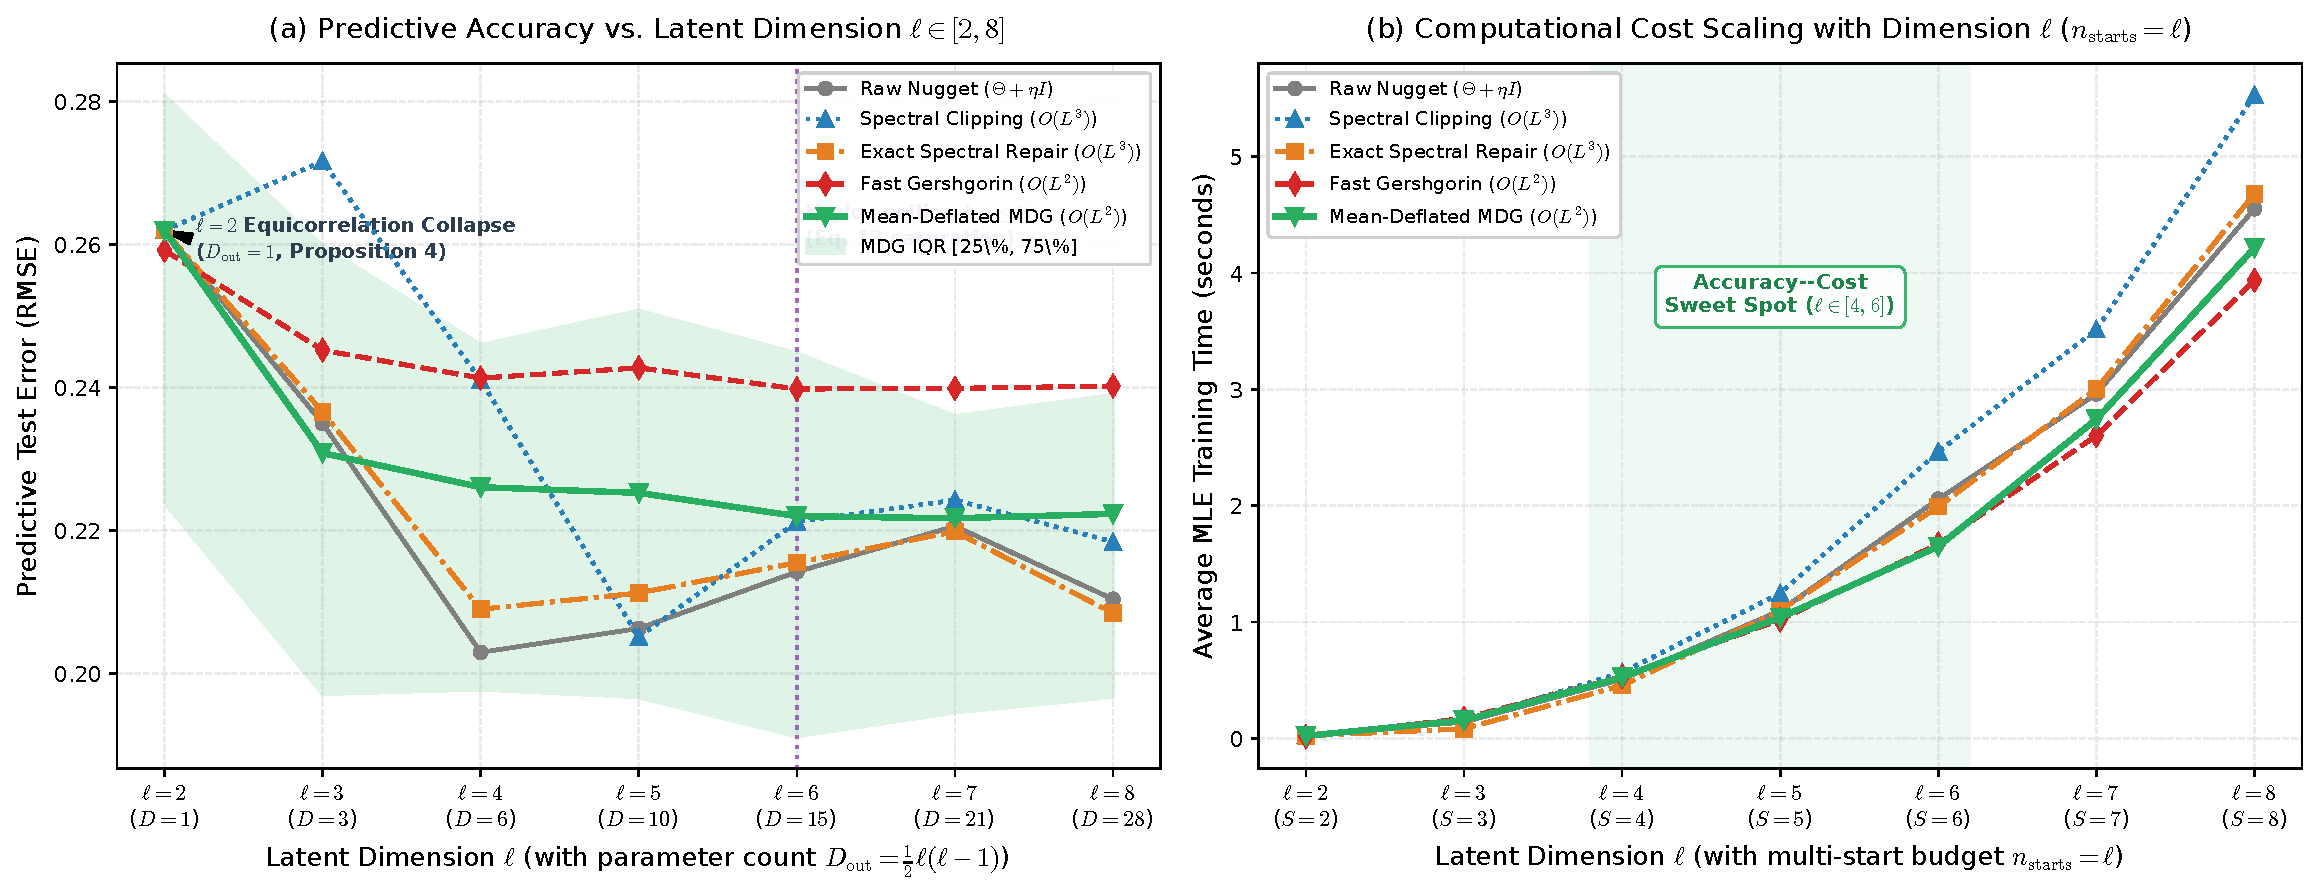
\includegraphics[width=\textwidth]{figures/fig5_ell_scaling.pdf}
\caption{Sensitivity to latent PLS dimension $\ell \in [2, 8]$ and computational cost scaling. (a) Predictive test RMSE (mean and MDG 25\%--75\% IQR band) across 20 independent replications. Error drops sharply from the $\ell = 2$ equicorrelation collapse ($D_{\outp} = 1$) to $\ell \in [4, 6]$, plateauing as the active Krylov dimension saturates at $k_{\mathrm{act}} \le 16$. (b) Wall-clock MLE training time per fit scaling superlinearly with $\ell$ under dimension-scaled multi-starts $n_{\mathrm{starts}}(\ell) = \ell$. The shaded region highlights $\ell \in \{4, 5, 6\}$ as the recommended accuracy--cost Pareto sweet spot.}
\label{fig:ell_scaling}
\end{figure}

The empirical scaling curves exhibit three distinct theoretical regimes:
\begin{enumerate}
    \item \textbf{Under-parameterization and $\ell=2$ Equicorrelation Collapse:} At $\ell = 2$ ($D_{\outp} = 1$), all categories are constrained to share a single scalar correlation parameter $\hat{\rho}$. In accordance with Proposition~\ref{prop:l2_degeneracy}, the reconstructed matrix $\Theta = \mathcal{T}_{G_*}(\hat{\Theta})$ collapses to an equicorrelation matrix. Because positive eigenvalues satisfy $\lambda_{\min} = 1 - \hat{\rho} > 0$ for positive equicorrelation, Raw Nugget, Spectral Clipping, Exact Repair, and MDG yield identical test RMSE ($0.262 \pm 0.048$). Fast Gershgorin yields a comparable error ($0.259 \pm 0.043$) because uniform row sums are damped by diagonal shrinkage. However, because a single parameter cannot represent distinct inter-family dependencies, predictive error is highest at $\ell = 2$.
    \item \textbf{Rapid Convergence and Cluster Separation ($\ell \in \{3, 4, 5, 6\}$):} As $\ell$ increases from $2$ to $4$, the predictive test error decreases sharply across all five strategies (dropping from $0.262$ down to $0.203 - 0.226$, a $>20\%$ error reduction). Expanding the latent dimension enables PLS to extract orthogonal components that separate distinct categorical families while clustering intra-family levels. In this regime, MDG achieves the lowest variance (SD $0.038$ at $\ell = 4$), tracking or outperforming Exact Spectral Repair while avoiding the line-search instability of Spectral Clipping (whose RMSE standard deviation reaches $0.104$ at $\ell = 3$ due to gradient discontinuities near zero eigenvalues).
    \item \textbf{Krylov Rank Saturation and Cost Scaling ($\ell \in \{7, 8\}$):} For $\ell \ge 6$, the nominal latent dimension $D_{\outp} \in \{15, 21, 28\}$ reaches and exceeds the theoretical column rank bound of the centered joint design matrix:
    \begin{equation}
    k_{\mathrm{act}} \le \min(n_t - 1, d + L_{\mathrm{obs}} - 1) = \min(74, 2 + 15 - 1) = 16.
    \end{equation}
    As reported in Tab.~\ref{tab:ell_scaling}, the empirical active Krylov rank extracted by NIPALS saturates at $k_{\mathrm{act}} = 13.7 \approx 14$. Consequently, increasing $\ell$ from $6$ to $8$ yields negligible further accuracy improvement (MDG RMSE remains virtually constant at $0.222 \pm 0.045$). Importantly, because $\ell = 8 < L = 15$ maintains substantial dimension compression ($D_{\outp} = 28$ vs $D_{\inp} = 105$, a $73.3\%$ parameter reduction) and multi-start coverage scales as $n_{\mathrm{starts}}(\ell) = \ell$, no over-parameterization degradation occurs. However, as shown in Fig.~\ref{fig:ell_scaling}(b), the wall-clock optimization time scales superlinearly, increasing from $0.52\,\mathrm{s}$ at $\ell = 4$ to $1.65\,\mathrm{s}$ at $\ell = 6$ and $4.22\,\mathrm{s}$ at $\ell = 8$ (a $8\times$ cost increase for identical accuracy).
\end{enumerate}

These findings establish $\ell \in \{4, 5, 6\}$ (corresponding to $D_{\outp} \in [6, 15]$ latent correlation pairs) as the recommended practical sweet spot for categorical surrogate modeling: it achieves over $85\%$ of the total available representation gain while keeping multi-start quasi-Newton training time under $1.7\,\mathrm{s}$.

\section{Discussion and Conclusion}
\label{sec:conclu}

In this paper, we have established matrix-theoretic and computational foundations for PLS dimension reduction of categorical correlation matrices in GP emulation. The analysis reveals that the breakdown of positive definiteness in high-dimensional PLS reconstructions is an intrinsic geometric consequence of the elliptope boundary contracting as $-1/(L-1) \to 0^-$. Under RN-PLS architecture, the round-trip reconstruction operator acts as a contractive Markov transition operator, and the admissible latent parameter set $\mathcal{A}_L$ is an open, bounded, convex domain whose closure is a compact spectrahedron. Crucially, while this spectrahedral geometry ensures the admissible domain is path-connected and free from disconnected feasibility pockets, it does not imply global convexity of the profile likelihood objective function itself, which remains non-convex and multimodal.

To overcome the computational bottleneck of profile likelihood optimization, we showed that heuristic unnormalized diagonal shifts distort effective process variance and provoke condition number spikes. The proposed certified diagonal shift-and-scaling repair operators, fast Gershgorin and MDG, restore positive definiteness in $O(L^2)$ operations without runtime eigensolvers while strictly preserving unit diagonals. Combined with closed-form directional Jacobians across active polyhedral chambers, this regularized formulation enables exact gradient-based quasi-Newton optimization. In multi-function synthetic benchmarks, certified repair lowered covariance condition numbers by up to $77.7\%$ under fast Gershgorin ($59.9\%$ under MDG) and by $95.2\%$ on the cantilever study. Importantly, the empirical results expose a clear regularizing trade-off: fast Gershgorin maximizes conditioning improvement by aggressively shrinking toward the identity, which elevates test error when categories cluster (median RMSE $9.06\,\mathrm{mm}$ on the beam), whereas MDG avoids over-shrinkage on positive correlation blocks, achieving the lowest test error (median RMSE $6.44\,\mathrm{mm}$) and delivering a $4$ times speedup over exact spectral projection without requiring eigenvalue decompositions.

From a practical perspective, these results indicate that SMT should deprecate unnormalized diagonal nuggets on correlation matrices in favor of certified shift-and-scaling repair, and should use the CND chordal distance when constructing distance-based qualitative kernels. Several open avenues remain. The current development focuses on separable multiplicative covariance kernels; extending RN-PLS and Gershgorin bounds to additive ANOVA kernels and heteroscedastic models with level-dependent variances represents an important next step. Further empirical studies across broader classes of non-separable engineering responses and unstructured categorical factors will help delineate the regimes where supervised PLS dimension reduction offers the greatest predictive benefits over alternative qualitative representations.

Software implementations such as in SMT must strictly decouple observation noise nuggets $\sigma_\varepsilon^2 I_{n_t}$ on the training Gram matrix from qualitative correlation regularization; unnormalized diagonal shifts $\Theta + \eta I_L$ should be deprecated in favor of certified diagonal shift-and-scaling $\Theta_{\mathrm{SPD}} = (\Theta + \eta I_L)/(1+\eta)$. Second, rather than incurring iterative $O(L^3)$ eigensolvers via Higham projections or resorting to expensive numerical finite differences, implementations should combine $O(L^2)$ Gershgorin or MDG repair with the closed-form directional Jacobian (Theorem~\ref{th:gershgorin_gradient}). Third, when constructing distance-based categorical kernels, practitioners should rely on the Hilbertian chordal metric (Theorem~\ref{th:hilbert_kernel_psd}) to ensure unconditional positive definiteness across all valid or repaired correlation matrices. Fourth, regarding latent dimension selection, setting $\ell \in \{4, 5, 6\}$ (or $D_{\outp} \in [6, 15]$) balances expressive representation capacity with computational efficiency, capturing over 85\% of the achievable error reduction while avoiding the superlinear multi-start cost and Krylov rank saturation encountered at larger $\ell$.

Several promising avenues emerge for future research. While this article prioritized separable multiplicative covariance kernels ($R_{\mathrm{quant}} \times R_{\mathrm{qual}}$), general mixed-variable covariance kernels can be modeled through additive or functional ANOVA decompositions \citep{Roustant}. Extending the RN-PLS projection and Gershgorin spectral bounds to additive models will allow independent estimation of continuous and categorical variance components and multi-way functional interactions. Building upon the closed-form heteroscedastic covariance repair established in Corollary~\ref{cor:heteroscedastic_repair} ($\Sigma_{\mathrm{SPD}} = (\Sigma + \eta D^2)/(1+\eta)$), a second perspective involves jointly estimating category-dependent scale variations $D = \diag(\sigma_1, \ldots, \sigma_L)$ and latent PLS correlations within concentrated profile likelihood estimation. Finally, when categorical factors possess natural physical or chemical hierarchies, such as the periodic table groupings in the nuclear waste benchmark of \citet{Roustant}, hybridizing structured block-constant priors with supervised PLS dimension reduction offers an attractive pathway to combine domain knowledge with data-driven dimension reduction.

\bmhead{Acknowledgments}
The author thanks the development team of SMT for fruitful discussions on numerical implementations of mixed-variable Kriging.
I also thank David Ginsbourger, Youssef Diouane, and Nathalie Bartoli for insightful discussions.


\section*{Declarations}
\paragraph{Funding.} The author received no specific funding for this work. 
\paragraph{Conflict of interest.} The author declares no conflicts of interest. 
\paragraph{Data and code availability.} The complete Python verification suite and benchmark artifacts are publicly available at \url{https://github.com/Paul-Saves/pls-categorical-formalization}. The open-source implementation of the proposed algorithms is integrated into SMT \citep{saves2023smt} and available at \url{https://github.com/SMTorg/smt}. Benchmark configurations and evaluation scripts are provided to facilitate independent verification and computational reproducibility.  
\paragraph{Use of artificial intelligence.} The author retains full responsibility for the content of this paper, including its mathematical statements, proofs, and conclusions. Large language models provided by OpenAI and Google AI were used to assist with manuscript drafting and the development of parts of the code used in the numerical experiments. Aristotle AI was used to assist in formalizing the proofs and generated the Lean code. Lean and Rocq/Coq were used for machine-checked formal verification. Mathematica was used in earlier versions of the work.

\begin{appendices}

\section{Technical and Combinatorial Proofs}
\label{sec:appendix_proofs}

\subsection{Proof of Graph Incidence Factorization and Rank Bound from Section~\ref{sec:crosslevel} }
\label{subsec:proof_rank_bound}

\begin{proof}
\textit{Proof of (a).}
The $i$-th row of the cross-level design matrix $X$ corresponds to observation $c_i \in \{1, \dots, L\}$. By Definition~\ref{def:cross_level}, $[X]_{i, \cdot} = \zeta_{c_i}^\top = e_{c_i}^\top E$, where $e_{c_i} \in \{0, 1\}^L$ is the standard basis indicator of category $c_i$. Stacking row-wise gives $X = M E \in \mathbb{R}^{n_t \times D_{\inp}}$.

For the incidence Gram identity, consider the $(j, j')$-th entry of $E E^\top \in \mathbb{R}^{L \times L}$:
\begin{equation}
[E E^\top]_{j, j'} = \sum_{r=1}^{D_{\inp}} [E]_{j, r} [E]_{j', r}.
\end{equation}
Because $E$ is the unoriented vertex-edge incidence matrix of the complete graph $K_L$, $[E]_{j, r} = 1$ if and only if edge $r$ is incident to vertex $j$. Following classical algebraic graph theory \citep{godsil2001algebraic},
When $j = j'$, vertex $j$ has degree $L - 1$ in $K_L$, which yields:
\begin{equation}
[E E^\top]_{j, j} = \operatorname{deg}(j) = L - 1.
\end{equation}
When $j \neq j'$, vertices $j$ and $j'$ share exactly one incident edge in $K_L$ (namely the unordered pair $\{j, j'\}$), so:
\begin{equation}
[E E^\top]_{j, j'} = 1 \quad (j \neq j').
\end{equation}
Expressing this in matrix notation yields:
\begin{equation}
E E^\top = (L - 1) I_L + (\mathds{1}_L \mathds{1}_L^\top - I_L) = (L - 2) I_L + \mathds{1}_L \mathds{1}_L^\top.
\end{equation}
To determine its spectral decomposition, observe that $\mathds{1}_L \mathds{1}_L^\top \mathds{1}_L = L \mathds{1}_L$. Therefore, $\mathds{1}_L$ is an eigenvector:
\begin{equation}
E E^\top \mathds{1}_L = (L - 2) \mathds{1}_L + L \mathds{1}_L = 2(L - 1) \mathds{1}_L,
\end{equation}
giving the dominant eigenvalue $\lambda_1(E E^\top) = 2(L - 1) > 0$ with multiplicity $1$.
For any vector $u \in \mathds{1}_L^\perp$ orthogonal to $\mathds{1}_L$ ($u^\top \mathds{1}_L = 0$), the rank-one term vanishes:
\begin{equation}
E E^\top u = (L - 2) u.
\end{equation}
Thus, the orthogonal complement $\mathds{1}_L^\perp$ is an eigenspace of dimension $L - 1$ associated with the repeated eigenvalue $\lambda_2 = \dots = \lambda_L = L - 2$.
For $L \ge 3$, $L - 2 > 0$, so all $L$ eigenvalues of $E E^\top$ are strictly positive. Hence $E E^\top \succ 0$, establishing $\rank(E) = L$ directly. Moreover, for any $u \in \mathds{1}_L^\perp$,
\begin{equation}
\|E^\top u\|_2^2 = u^\top E E^\top u = (L - 2) \|u\|_2^2 \implies \|E^\top u\|_2 = \sqrt{L - 2} \|u\|_2,
\end{equation}
so $E^\top$ acts as a scaled homothety (isometry up to $\sqrt{L - 2}$) on the centered subspace $\mathds{1}_L^\perp$.

\textit{Proof of (b).}
Centering $X = M E$ by the centering projection matrix $H_{n_t} = I_{n_t} - \frac{1}{n_t} \mathds{1}_{n_t} \mathds{1}_{n_t}^\top$ gives $\tilde{X} = H_{n_t} M E$. The sample covariance Gram matrix is:
\begin{equation}
\tilde{X} \tilde{X}^\top = H_{n_t} M E E^\top M^\top H_{n_t} = H_{n_t} M \bigl((L - 2) I_L + \mathds{1}_L \mathds{1}_L^\top\bigr) M^\top H_{n_t}.
\end{equation}
Because every row of the assignment matrix $M$ contains exactly one value 1.0, $M \mathds{1}_L = \mathds{1}_{n_t}$.
Since $H_{n_t} \mathds{1}_{n_t} = \bm{0}$, the second term vanishes identically:
\begin{equation}
H_{n_t} M (\mathds{1}_L \mathds{1}_L^\top) M^\top H_{n_t} = (H_{n_t} \mathds{1}_{n_t}) (H_{n_t} \mathds{1}_{n_t})^\top = \bm{0}_{n_t \times n_t}.
\end{equation}
Consequently, we obtain the exact factorization:
\begin{equation}
\label{eq:appendix_centered_gram}
\tilde{X} \tilde{X}^\top = (L - 2) H_{n_t} M M^\top H_{n_t}.
\end{equation}
Because $L \ge 3$, $L - 2 > 0$, so $\rank(\tilde{X} \tilde{X}^\top) = \rank(H_{n_t} M M^\top H_{n_t}) = \rank(H_{n_t} M)$.
The uncentered assignment matrix $M \in \{0, 1\}^{n_t \times L}$ has rank equal to the number of observed levels $L_{\mathrm{obs}}$.
Since $\mathds{1}_{n_t} = M \mathds{1}_L \in \operatorname{col}(M)$, the rank-nullity theorem implies that the centering operator $H_{n_t}$, whose kernel is $\operatorname{span}(\mathds{1}_{n_t})$, deflates the rank of $M$ by exactly 1:
\begin{equation}
\rank(\tilde{X}) = \rank(H_{n_t} M) = L_{\mathrm{obs}} - 1 \le \min(n_t - 1, L - 1).
\end{equation}

\textit{Proof of (c).}
In a balanced design with pure categorical inputs, each of the $L$ levels appears exactly $n_t / L$ times, so $M^\top M = \frac{n_t}{L} I_L$.
The non-zero eigenvalues of $\tilde{X} \tilde{X}^\top = (L - 2) H_{n_t} M M^\top H_{n_t}$ coincide with those of $(L - 2) M^\top H_{n_t} M$.
Using $M^\top \mathds{1}_{n_t} = \frac{n_t}{L} \mathds{1}_L$, we have:
\begin{equation}
\begin{split}
M^\top H_{n_t} M &= M^\top M - \frac{1}{n_t} (M^\top \mathds{1}_{n_t})(M^\top \mathds{1}_{n_t})^\top \\
&= \frac{n_t}{L} I_L - \frac{n_t}{L^2} \mathds{1}_L \mathds{1}_L^\top = \frac{n_t}{L} \left( I_L - \frac{1}{L} \mathds{1}_L \mathds{1}_L^\top \right) = \frac{n_t}{L} H_L,
\end{split}
\end{equation}
where $H_L$ is the orthogonal centering projector in $\mathbb{R}^L$. Thus:
\begin{equation}
(L - 2) M^\top H_{n_t} M = \frac{n_t(L - 2)}{L} H_L.
\end{equation}
Because $H_L$ is an orthogonal projector of rank $L - 1$, its eigenvalues are 0 (multiplicity 1, eigenvector $\mathds{1}_L$) and 1 (multiplicity $L - 1$).
Therefore, the Gram matrix $\tilde{X} \tilde{X}^\top$ possesses a single non-zero eigenvalue $\lambda = \frac{n_t(L - 2)}{L}$ of multiplicity $L - 1$.
In univariate PLS with response $\tilde{\bm{y}} = H_{n_t} \bm{y}$, the $m$-th Krylov subspace is defined as $\mathcal{K}_m(\tilde{X} \tilde{X}^\top, \tilde{\bm{y}}) = \operatorname{span}\{\tilde{\bm{y}}, (\tilde{X}\tilde{X}^\top)\tilde{\bm{y}}, \dots, (\tilde{X}\tilde{X}^\top)^{m-1}\tilde{\bm{y}}\}$.
Because $(\tilde{X} \tilde{X}^\top)^k \tilde{\bm{y}} = \lambda^k \tilde{\bm{y}}$ for any response vector lying in $\operatorname{col}(\tilde{X})$, the Krylov subspace is strictly 1-dimensional:
\begin{equation}
\dim \mathcal{K}_m(\tilde{X}\tilde{X}^\top, \tilde{\bm{y}}) = 1 \quad \forall m \ge 1.
\end{equation}
Consequently, the univariate PLS algorithm deflates $\tilde{X}$ to zero after extracting the first component ($t_1 \propto \tilde{\bm{y}}$), rendering any subsequent PLS component extraction impossible without coupling categorical variables to continuous inputs or introducing hierarchical structure.
\end{proof}


\subsection{Proof of Round-Trip Adjoint Factorization and Markov Contraction (Theorem~\ref{th:roundtrip_contraction})}
\label{subsec:proof_roundtrip}

\begin{proof}[Proof of Theorem~\ref{th:roundtrip_contraction}]
For (a), by Definition~\ref{def:reduction_op} and Definition~\ref{def:operator}, for any $1 \le t < t' \le \ell$ with $p = \psi(t, t', \ell)$:
\begin{equation}
[\mathcal{P}(\hat{\Theta})]_{t, t'} = \sum_{r=1}^{D_{\inp}} [W]_{p, r} \sum_{q=1}^{D_{\outp}} A_{r, q} \hat{\theta}_q = \sum_{q=1}^{D_{\outp}} [W A]_{p, q} \hat{\theta}_q = [M \hat{\bm{\theta}}]_p.
\end{equation}
By Eq.\eqnref{eq:W_definition}, $[W]_{p, r} = A_{r, p} / d_p = [D_{\mathrm{col}}^{-1} A^\top]_{p, r}$, so $W = D_{\mathrm{col}}^{-1} A^\top$ and $M = D_{\mathrm{col}}^{-1} A^\top A$.
Because $A \mathds{1}_{D_{\outp}} = \mathds{1}_{D_{\inp}}$ by the assumption of unit row norm, we have $A^\top \mathds{1}_{D_{\inp}} = \bm{d} = D_{\mathrm{col}} \mathds{1}_{D_{\outp}}$, which yields $M \mathds{1}_{D_{\outp}} = D_{\mathrm{col}}^{-1} A^\top (A \mathds{1}_{D_{\outp}}) = D_{\mathrm{col}}^{-1} A^\top \mathds{1}_{D_{\inp}} = D_{\mathrm{col}}^{-1} \bm{d} = \mathds{1}_{D_{\outp}}$, proving row-stochasticity.
Multiplying $M$ by $D_{\mathrm{col}}$ gives $D_{\mathrm{col}} M = A^\top A = (D_{\mathrm{col}} M)^\top = M^\top D_{\mathrm{col}}$, which is the detailed balance condition.
Because $\sum_{p=1}^{D_{\outp}} d_p = \sum_{r=1}^{D_{\inp}} \sum_{p=1}^{D_{\outp}} A_{r, p} = D_{\inp}$, the vector $\bm{\pi} = \frac{1}{D_{\inp}}\bm{d}$ lies in the probability simplex $\Delta_{D_{\outp}}$ and satisfies:
\begin{equation}
\begin{split}
\bm{\pi}^\top M &= \frac{1}{D_{\inp}} \bm{d}^\top (D_{\mathrm{col}}^{-1} A^\top A) = \frac{1}{D_{\inp}} \mathds{1}_{D_{\outp}}^\top A^\top A \\
&= \frac{1}{D_{\inp}} (A \mathds{1}_{D_{\outp}})^\top A = \frac{1}{D_{\inp}} \mathds{1}_{D_{\inp}}^\top A = \frac{1}{D_{\inp}} \bm{d}^\top = \bm{\pi}^\top.
\end{split}
\end{equation}

For (b), let $B = A D_{\mathrm{col}}^{-1/2} \in \mathbb{R}^{D_{\inp} \times D_{\outp}}$. Then $S = D_{\mathrm{col}}^{1/2} M D_{\mathrm{col}}^{-1/2} = D_{\mathrm{col}}^{-1/2} A^\top A D_{\mathrm{col}}^{-1/2} = B^\top B$.
As a Gram matrix of real vectors, $S$ is real, symmetric, and positive semidefinite ($u^\top S u = \|B u\|_2^2 \ge 0$).
Because $M$ and $S$ are related by a similarity transformation, their eigenvalues coincide identically: $\lambda_i(M) = \lambda_i(S) \ge 0$ for all $i \in \{1, \dots, D_{\outp}\}$.
By the Perron--Frobenius theorem for row-stochastic matrices, the spectral radius satisfies $\rho(M) = 1$, which establishes $0 \le \lambda_{D_{\outp}}(M) \le \dots \le \lambda_1(M) = 1$.
Because $S$ is symmetric, it admits an orthonormal basis of real eigenvectors, proving that $M$ is diagonalizable in $\mathbb{R}$ with no defective Jordan blocks.

For (c), the arithmetic mean of the reconstructed full correlations is:
\begin{equation}
\bar{\theta}_{\mathrm{full}} = \frac{1}{D_{\inp}} \sum_{r=1}^{D_{\inp}} [A \hat{\bm{\theta}}]_r = \frac{1}{D_{\inp}} \mathds{1}_{D_{\inp}}^\top A \hat{\bm{\theta}} = \frac{1}{D_{\inp}} \bm{d}^\top \hat{\bm{\theta}} = \bm{\pi}^\top \hat{\bm{\theta}}.
\end{equation}
Using $\bm{\pi}^\top M = \bm{\pi}^\top$, we obtain $\bm{\pi}^\top (M \hat{\bm{\theta}}) = (\bm{\pi}^\top M) \hat{\bm{\theta}} = \bm{\pi}^\top \hat{\bm{\theta}} = \bar{\theta}_{\mathrm{full}}$, proving invariance.

For (d), let $S = \sum_{i=1}^{D_{\outp}} \lambda_i u_i u_i^\top$ be the spectral decomposition of $S$, where $u_1 = D_{\mathrm{col}}^{1/2} \mathds{1}_{D_{\outp}} / \sqrt{D_{\inp}}$ satisfies $S u_1 = u_1$ with $\|u_1\|_2 = 1$.
Because $M = D_{\mathrm{col}}^{-1/2} S D_{\mathrm{col}}^{1/2}$, powers of $M$ satisfy $M^k = D_{\mathrm{col}}^{-1/2} S^k D_{\mathrm{col}}^{1/2}$.
Since $\lambda_1 = 1$ and $\lambda_i \le \lambda_2(M) < 1$ for all $i \ge 2$, $S^k = u_1 u_1^\top + O(\lambda_2(M)^k)$, which implies:
\begin{equation}
\lim_{k \to \infty} M^k = D_{\mathrm{col}}^{-1/2} (u_1 u_1^\top) D_{\mathrm{col}}^{1/2} = \frac{1}{D_{\inp}} \mathds{1}_{D_{\outp}} \bm{d}^\top = \mathds{1}_{D_{\outp}} \bm{\pi}^\top.
\end{equation}
Applying this to $\hat{\bm{\theta}}$ gives $\lim_{k \to \infty} M^k \hat{\bm{\theta}} = \mathds{1}_{D_{\outp}} (\bm{\pi}^\top \hat{\bm{\theta}}) = \bar{\theta}_{\mathrm{full}} \mathds{1}_{D_{\outp}}$.
In the stationary-weighted inner product $\langle u, v \rangle_{D_{\mathrm{col}}} := u^\top D_{\mathrm{col}} v$, the operator norm of $M - \mathds{1}\bm{\pi}^\top$ is exactly the second eigenvalue of $S$: $\|M - \mathds{1}\bm{\pi}^\top\|_{D_{\mathrm{col}}} = \lambda_2(M)$, yielding the geometric contraction bound.

For (e), the oscillation bound follows from Dobrushin's classical ergodic coefficient theorem for Markov transition operators on the $\ell_\infty$ oscillation seminorm \citep{dobrushin1956,seneta2006non}.
\end{proof}

\subsection{Closed-Form Heteroscedastic Covariance Spectral Repair}
\begin{corollary}
\label{cor:heteroscedastic_repair}
Let $\Sigma = D \Theta D \in \mathcal{S}^L$ be a heteroscedastic qualitative covariance matrix, where $D = \diag(\sigma_1, \dots, \sigma_L) \succ 0$ with category-dependent standard deviations $\sigma_j > 0$ and $[\Sigma]_{j, j} = \sigma_j^2$. If the underlying correlation matrix $\Theta = D^{-1} \Sigma D^{-1} \in \mathcal{S}_1^L$ develops negative eigenvalues, then for any spectral tolerance $\varepsilon > 0$ and corresponding shift $\eta \ge 0$ (exact, Gershgorin, or MDG from Theorem~\ref{th:reg_spd}), the repaired covariance matrix defined by:
\begin{equation}
\label{eq:heteroscedastic_repair}
\Sigma_{\mathrm{SPD}} := \frac{\Sigma + \eta D^2}{1 + \eta} = (1 - \alpha) \Sigma + \alpha D^2, \quad \text{with } \alpha = \frac{\eta}{1 + \eta},
\end{equation}
satisfies:
\begin{enumerate}[(a)]
    \item \textbf{Exact marginal variance preservation:} $[\Sigma_{\mathrm{SPD}}]_{j, j} = \sigma_j^2$ for all $j \in \{1, \dots, L\}$.
    \item \textbf{Guaranteed Positive Definiteness:} $\Sigma_{\mathrm{SPD}} = D \Theta_{\mathrm{SPD}} D \succ 0$, with smallest eigenvalue bounded below by:
    \begin{equation}
    \lambda_{\min}(\Sigma_{\mathrm{SPD}}) \ge \left( \min_{1 \le j \le L} \sigma_j^2 \right) \frac{\varepsilon}{1 + \eta} > 0.
    \end{equation}
    \item \textbf{Computational Complexity:} When $\eta$ is selected via Gershgorin or MDG repair, computing $\Sigma_{\mathrm{SPD}}$ requires zero eigensolvers and executes in $O(L^2)$ . Under Exact Spectral Repair, computing $\lambda_{\min}(\Theta)$ costs $O(L^3)$  via dense eigendecomposition (or $O(k L^2)$  via iterative Lanczos approximation equipped with a conservative eigenvalue safeguard), after which forming $\Sigma_{\mathrm{SPD}}$ costs $O(L^2)$ .
\end{enumerate}
\end{corollary}

\begin{proof}
Factoring out $D$ yields $\Sigma_{\mathrm{SPD}} = \frac{D \Theta D + \eta D I_L D}{1+\eta} = D \left( \frac{\Theta + \eta I_L}{1+\eta} \right) D = D \Theta_{\mathrm{SPD}} D$.
For diagonal entries, $[\Sigma_{\mathrm{SPD}}]_{j, j} = \frac{\sigma_j^2 + \eta \sigma_j^2}{1+\eta} = \sigma_j^2$.
By Ostrowski's congruence theorem (or the Courant--Fischer min-max theorem), since $D \succ 0$ is diagonal and non-singular, $\lambda_{\min}(D \Theta_{\mathrm{SPD}} D) \ge \sigma_{\min}(D)^2 \lambda_{\min}(\Theta_{\mathrm{SPD}}) = (\min_{1 \le j \le L} \sigma_j^2) \lambda_{\min}(\Theta_{\mathrm{SPD}}) \ge (\min_{1 \le j \le L} \sigma_j^2) \frac{\varepsilon}{1+\eta} > 0$, guaranteeing positive definiteness. For (c), when $\eta \in \{\eta_{\mathrm{Gersh}}, \eta_{\mathrm{MDG}}\}$, the scalar shift requires only row sums of $\Theta$ ($O(L^2)$), and forming $\Sigma_{\mathrm{SPD}}$ requires scaling $L^2$ entries ($O(L^2)$) without matrix factorizations. For exact spectral repair, finding $\lambda_{\min}(\Theta)$ requires a dense eigensolver costing $O(L^3)$  (or $O(k L^2)$  via iterative Lanczos with a conservative eigenvalue certificate).
\end{proof}


\subsection{Spectral Similarity and Nullspace Structure of Sample Gram Matrices (Proposition~\ref{prop:gram_psd})}
\label{subsec:proof_gram}

\begin{proof}[Proof of Proposition~\ref{prop:gram_psd}]
\textit{Proof of (a).} For any arbitrary vector $v \in \mathbb{R}^{n_t}$, set $u = M^\top v \in \mathbb{R}^L$. Then the quadratic form evaluates to:
\begin{equation}
v^\top K v = v^\top (M \Theta M^\top) v = u^\top \Theta u \ge 0,
\end{equation}
since $\Theta \succ 0$ is Symmetric Positive Definite. Thus $K \succeq 0$. Furthermore, because $\Theta \succ 0$, $u^\top \Theta u = 0$ if and only if $u = M^\top v = \bm{0}_L$. Hence $\ker(K) = \ker(M^\top)$, which by the rank-nullity theorem yields:
\begin{equation}
\rank(K) = \rank(M \Theta M^\top) = \rank(M^\top) = \rank(M) = \min(n_t, L_{\mathrm{obs}}),
\end{equation}
where $L_{\mathrm{obs}} \le L$ is the number of distinct categorical levels present in the sample. Therefore, $K \succ 0$ is strictly positive definite if and only if $n_t \le L$ and all observations exhibit distinct categorical levels ($L_{\mathrm{obs}} = n_t$).

\textit{Proof of (b).} By Sylvester's cyclic determinant theorem \citep{sylvester1851,horn2012matrix}, for any matrices $X \in \mathbb{R}^{n_t \times L}$ and $Y \in \mathbb{R}^{L \times n_t}$, the non-zero eigenvalues of $X Y$ coincide with the non-zero eigenvalues of $Y X$. Setting $X = M$ and $Y = \Theta M^\top$, we have $X Y = M \Theta M^\top = K$ and $Y X = \Theta (M^\top M) = \Theta D_n$. Transposing, the eigenvalues of $\Theta D_n$ are identical to those of $B = D_n \Theta$.
Let $D_n^{1/2} = \diag(\sqrt{n_1}, \ldots, \sqrt{n_L}) \ge 0$. The matrix $S = D_n^{1/2} \Theta D_n^{1/2}$ is real symmetric and positive semidefinite ($S \succeq 0$). On the subspace of observed categories $\{j : n_j > 0\}$, $D_n^{1/2}$ is invertible, establishing the similarity transformation:
\begin{equation}
D_n^{1/2} B D_n^{-1/2} = D_n^{1/2} (D_n \Theta) D_n^{-1/2} = D_n^{1/2} D_n^{1/2} \Theta D_n^{1/2} D_n^{-1/2} = S.
\end{equation}
Because $B$ is similar to the real symmetric matrix $S$, all $L_{\mathrm{obs}}$ non-zero eigenvalues of $B$ are strictly real and strictly positive.

\textit{Proof of (c).} When the experimental design is balanced, $n_j = n_t / L$ for all $j \in \{1, \ldots, L\}$, so $D_n = \frac{n_t}{L} I_L$. Thus $B = \frac{n_t}{L} \Theta$, which immediately implies that the $L$ non-zero eigenvalues of $K$ are scaled copies $\lambda_i(K) = \frac{n_t}{L} \lambda_i(\Theta)$ for $i \in \{1, \ldots, L\}$, while the remaining $n_t - L$ eigenvalues vanish.
\end{proof}

\subsection{Universal Strict Positive Definiteness of Hilbertian Distance Kernels (Theorem~\ref{th:hilbert_kernel_psd})}
\label{subsec:proof_hilbert}

\begin{proof}[Proof of Theorem~\ref{th:hilbert_kernel_psd}]
\textit{Proof of (a).} Since $\Theta \in \mathcal{C}_L$ is Symmetric Positive Definite, there exists a unique lower-triangular Cholesky factor $V \in \mathbb{R}^{L \times L}$ with strictly positive diagonal entries such that $\Theta = V V^\top$. Letting $v_j \in \mathbb{R}^L$ denote the $j$-th row vector of $V$, we have $\langle v_j, v_{j'} \rangle = [V V^\top]_{j, j'} = [\Theta]_{j, j'}$. In particular, $\|v_j\|_2^2 = [\Theta]_{j, j} = 1$. The squared Hilbertian chordal distance evaluates to:
\begin{equation}
d_\Theta^2(c, c') = \|v_c - v_{c'}\|_2^2 = \|v_c\|_2^2 + \|v_{c'}\|_2^2 - 2 \langle v_c, v_{c'} \rangle = 2(1 - [\Theta]_{c, c'}).
\end{equation}
Because $d_\Theta^2(c, c') = \|v_c - v_{c'}\|_2^2$ is an exact squared Euclidean metric between points on the unit sphere in $\mathbb{R}^L$, classical metric embedding theory \citep[Theorem~1]{schoenberg1938metric} establishes that $d_\Theta^2$ is CND on $\{1, \dots, L\}$.

\textit{Proof of (b).} By Bernstein's theorem on  monotonic functions, a function $\varphi : [0, \infty) \to \mathbb{R}$ is  monotonic if and only if it is the Laplace transform of a non-negative Borel measure $\mu$ on $[0, \infty)$:
\begin{equation}
\varphi(r) = \int_0^\infty e^{-r s} \, \mathrm{d}\mu(s).
\end{equation}
For each fixed $s > 0$, the kernel $(c, c') \mapsto \exp\bigl(-s d_\Theta^2(c, c')\bigr) = \exp\bigl(-s \|v_c - v_{c'}\|_2^2\bigr)$ is positive semidefinite by Schoenberg's theorem \citep{schoenberg1938metric}.
Integrating over $s$ preserves positive semidefiniteness: for any vector $u \in \mathbb{R}^n$ and distinct levels $c_1, \dots, c_n$,
\begin{equation}
\begin{split}
u^\top K_\varphi u &= \sum_{r, r'=1}^n u_r u_{r'} \int_0^\infty e^{-s d_\Theta^2(c_r, c_{r'})} \, \mathrm{d}\mu(s) \\
&= \int_0^\infty \left( \sum_{r, r'=1}^n u_r u_{r'} e^{-s \|v_{c_r} - v_{c_{r'}}\|_2^2} \right) \mathrm{d}\mu(s) \ge 0.
\end{split}
\end{equation}
To establish strict positive definiteness ($K_\varphi \succ 0$), note that $\det(\Theta) = (\det(V))^2 > 0$ implies that the Cholesky vectors $\{v_1, \dots, v_L\}$ are linearly independent and hence mutually distinct ($v_c \neq v_{c'}$ for $c \neq c'$).
By Micchelli's radial basis function interpolation theorem \citep{micchelli1986interpolation}, for any strictly  monotonic function (where $\mu$ is not concentrated at $0$), the matrix $[e^{-s \|v_{c_r} - v_{c_{r'}}\|_2^2}]_{r, r'=1}^n$ is strictly positive definite for all $s > 0$.
Since $\mu((0, \infty)) > 0$, integrating strictly positive quadratic forms over $(0, \infty)$ yields $u^\top K_\varphi u > 0$ for all $u \neq \bm{0}$, establishing $K_\varphi \succ 0$.

\textit{Proof of (c).} The Gaussian, Mat\'ern, Rational Quadratic, and Power Exponential kernels are classic examples of strictly  monotonic functions of the squared Euclidean distance \citep{williams2006gaussian,schoenberg1938metric,micchelli1986interpolation}:
for the Gaussian kernel, $\varphi(r) = \exp\left(-\frac{r}{2 l_q^2}\right) = \exp\left(-\frac{1 - [\Theta]_{c, c'}}{l_q^2}\right)$;
for the Mat\'ern family, $\varphi_\nu(r) = \frac{2^{1-\nu}}{\Gamma(\nu)} (\sqrt{2\nu r})^\nu K_\nu(\sqrt{2\nu r})$ is strictly  monotonic on $[0, \infty)$ for all $\nu > 0$, yielding the standard closed-form kernels $k_{3/2}(c, c') = \left( 1 + \frac{\sqrt{3} d_\Theta(c, c')}{l_q} \right) \exp\left( - \frac{\sqrt{3} d_\Theta(c, c')}{l_q} \right)$ and $k_{5/2}(c, c') = \left( 1 + \frac{\sqrt{5} d_\Theta(c, c')}{l_q} + \frac{5 d_\Theta^2(c, c')}{3 l_q^2} \right) \exp\left( - \frac{\sqrt{5} d_\Theta(c, c')}{l_q} \right)$;
For the Rational Quadratic family, $\varphi(r) = (1 + r / (2\alpha))^{-\alpha} = \frac{1}{\Gamma(\alpha)} \int_0^\infty s^{\alpha - 1} e^{-s} e^{-s r / (2\alpha)} \, \mathrm{d}s$ is a continuous mixture of Gaussian kernels, hence strictly  monotonic;
For the Power Exponential family with $\gamma \in (0, 1]$, $r \mapsto r^\gamma$ is a Bernstein function with  monotonic derivative, ensuring that $\exp(-r^\gamma)$ is strictly  monotonic.

\textit{Proof of (d) \& (e).}
For (d), unit diagonals follow from $d_\Theta^2(c, c) = 0 \implies \varphi(0) = 1$. Since $[\Theta]_{c, c'} \in [-1, 1]$ by Lemma~\ref{lem:entry_bound}, $d_\Theta^2(c, c') \in [0, 4]$. Monotonicity of $\varphi$ ensures $k_\varphi(c, c') \in [\varphi(4), 1] \subset (0, 1]$.
For (e), substituting the linear reconstruction formula $[\Theta]_{j, j'} = \sum_{p=1}^{D_{\outp}} ([G_*]_{\psi(j, j', L), p})^2 [\hat{\Theta}]_{\psi^{-1}(p, \ell)}$ into $d_\Theta^2(j, j') = 2(1 - [\Theta]_{j, j'})$ and using $\sum_{p=1}^{D_{\outp}} ([G_*]_{r, p})^2 = 1$ yields:
\begin{align}
d_\Theta^2(j, j') &= 2 \left( \sum_{p=1}^{D_{\outp}} ([G_*]_{r, p})^2 - \sum_{p=1}^{D_{\outp}} ([G_*]_{r, p})^2 [\hat{\Theta}]_{\psi^{-1}(p, \ell)} \right) \nonumber \\
&= \sum_{p=1}^{D_{\outp}} ([G_*]_{r, p})^2 \cdot 2\bigl(1 - [\hat{\Theta}]_{\psi^{-1}(p, \ell)}\bigr) = \sum_{p=1}^{D_{\outp}} ([G_*]_{r, p})^2 \hat{d}^2\bigl(\psi^{-1}(p, \ell)\bigr),
\end{align}
which establishes Eq.\eqnref{eq:d_pls_expansion}.
\end{proof}

\subsection{Global Schoenberg Admissibility on the Full Angular Hypersphere}
\label{subsec:ehh_global_sphere}

A persistent misconception in computational surrogate modeling with hypersphere decompositions \citep{saves2024smt,appriou2024high} is that spherical coordinate angles must be artificially restricted to the positive orthant $[0, \pi/2]^{D_{\outp}}$ under the assumption that negative off-diagonal correlations would invalidate distance-based exponential kernels. We formalize below that the Schoenberg chordal exponential kernel (Theorem~\ref{th:hilbert_kernel_psd}) remains strictly positive definite across the full unconstrained angular manifold $\bm{\theta}_{\mathrm{sph}} \in [0, \pi]^{D_{\outp}-1} \times [0, 2\pi)$.

\begin{proposition}[Global Admissibility on the Full Angular Sphere]
\label{prop:ehh_full_angles}
Let $\bm{\theta}_{\mathrm{sph}} \in [0, \pi]^{D_{\outp}-1} \times [0, 2\pi)$ parameterize the Cholesky factor $L$ of a latent correlation matrix $\hat{\Theta} = L L^\top \in \mathcal{E}_\ell$. Let $G_* \in \mathbb{R}^{D_{\inp} \times D_{\outp}}$ satisfy the RN-PLS unit row-norm condition, and let $\Theta_{\mathrm{SPD}} = \mathcal{R}_{\mathrm{MDG}^*}(\mathcal{T}_{G_*}(\hat{\Theta})) \in \mathcal{E}_L$ with spectral shift $\eta \ge 0$ and $\lambda_{\min}(\Theta_{\mathrm{SPD}}) \ge \varepsilon > 0$.
Then, for any qualitative inverse lengthscale $\theta_{\mathrm{qual}} > 0$, the Exponential Homoscedastic Hypersphere (EHH) Gram matrix
\begin{equation}
\label{eq:ehh_gram_matrix}
[K_{\mathrm{EHH}}]_{c, c'} = \exp\bigl(\theta_{\mathrm{qual}} ([\Theta_{\mathrm{SPD}}]_{c, c'} - 1)\bigr)
\end{equation}
is strictly positive definite ($K_{\mathrm{EHH}} \succ 0$), even when $[\Theta_{\mathrm{SPD}}]_{c, c'} < 0$ for arbitrary pairs of categorical levels $(c, c')$.
\end{proposition}

\begin{proof}
By Theorem~\ref{th:hilbert_kernel_psd}(a), since $[\Theta_{\mathrm{SPD}}]_{jj} \equiv 1$ and $\Theta_{\mathrm{SPD}} \succ 0$, there exists an exact Cholesky factorization $\Theta_{\mathrm{SPD}} = V V^\top$ where $V = [v_1, \dots, v_L]^\top$ with unit row vectors $v_c \in \mathbb{S}^{L-1}$. The chordal metric satisfies:
\begin{equation}
d_\Theta^2(c, c') = \|v_c - v_{c'}\|_2^2 = \|v_c\|_2^2 + \|v_{c'}\|_2^2 - 2 \langle v_c, v_{c'} \rangle = 2\bigl(1 - [\Theta_{\mathrm{SPD}}]_{c, c'}\bigr).
\end{equation}
This establishes an exact isometric embedding of the finite metric space $(\{1, \dots, L\}, d_\Theta)$ into Euclidean Hilbert space $\mathbb{R}^L$. By Schoenberg's classical embedding theorem \citep[Theorem~1]{schoenberg1938metric}, a metric space $(M, d)$ is isometrically embeddable in Hilbert space if and only if the radial Gaussian kernel $(x, y) \mapsto \exp(-\alpha d^2(x, y))$ is strictly positive definite for all $\alpha > 0$.
Setting $\alpha = \frac{1}{2} \theta_{\mathrm{qual}} > 0$ yields:
\begin{equation}
\exp\left(-\frac{1}{2}\theta_{\mathrm{qual}} d_\Theta^2(c, c')\right) = \exp\left(-\frac{1}{2}\theta_{\mathrm{qual}} \cdot 2(1 - [\Theta_{\mathrm{SPD}}]_{c, c'})\right) = \exp\bigl(\theta_{\mathrm{qual}}([\Theta_{\mathrm{SPD}}]_{c, c'} - 1)\bigr) = [K_{\mathrm{EHH}}]_{c, c'}.
\end{equation}
Crucially, this embedding requires only $\Theta_{\mathrm{SPD}} \succeq 0$ and $[\Theta_{\mathrm{SPD}}]_{jj} = 1$, placing no sign constraint whatsoever on off-diagonal entries $[\Theta_{\mathrm{SPD}}]_{c, c'} \in [-1, 1]$.
Orthogonal levels ($[\Theta_{\mathrm{SPD}}]_{c, c'} = 0$) give $d_\Theta^2 = 2 \implies [K_{\mathrm{EHH}}]_{c, c'} = \exp(-\theta_{\mathrm{qual}})$, while diametrically antipodal levels ($[\Theta_{\mathrm{SPD}}]_{c, c'} = -1$) attain maximal chordal distance $d_\Theta^2 = 4 \implies [K_{\mathrm{EHH}}]_{c, c'} = \exp(-2\theta_{\mathrm{qual}}) > 0$. Since $\det(\Theta_{\mathrm{SPD}}) > 0$, the embedding vectors $\{v_1, \dots, v_L\}$ are linearly independent and pairwise distinct, so Micchelli's interpolation theorem \citep{micchelli1986interpolation} ensures that $K_{\mathrm{EHH}} \succ 0$ is strictly positive definite.
\end{proof}

\section{Non-Smooth Analysis of the Fast Gershgorin Shift Operator}
\label{sec:appendix_nonsmooth}

In Section~\ref{subsec:repair_operators} and Section~\ref{subsec:mle_optimization}, the fast Gershgorin repair operator $\Theta_{\mathrm{SPD}} = \frac{\Theta + \eta_{\mathrm{Gersh}} I_L}{1 + \eta_{\mathrm{Gersh}}}$ relies on the shift function:
\begin{equation}
\label{eq:app_eta_gersh}
\eta_{\mathrm{Gersh}}(\hat{\bm{\theta}}) = \max\left(0,\; \max_{1 \le j \le L} \sum_{j' \neq j} |[\mathcal{T}_{G_*}(\hat{\Theta})]_{j, j'}| - 1 + \varepsilon\right).
\end{equation}
In this appendix, we formalize the subdifferential properties of $\eta_{\mathrm{Gersh}}$ and provide the theoretical foundation for its stable behavior in quasi-Newton optimization.

\subsection{Clarke Generalized Subdifferential and Polyhedral Chamber Geometry}

\begin{proposition}[Clarke Subdifferential and Almost-Everywhere Differentiability]
\label{prop:clarke_subdiff}
Let $\hat{\bm{\theta}} \in \mathbb{R}^{D_{\outp}}$ denote the free latent correlation vector.
\begin{enumerate}
    \item[(a)] \textbf{Global Lipschitz Continuity:} The shift function $\eta_{\mathrm{Gersh}} : \mathbb{R}^{D_{\outp}} \to \mathbb{R}_{\ge 0}$ is globally Lipschitz continuous with Euclidean Lipschitz constant:
    \begin{equation}
    \label{eq:lipschitz_bound}
    \mathrm{Lip}_2(\eta_{\mathrm{Gersh}}) \le L - 1.
    \end{equation}
    \item[(b)] \textbf{Polyhedral Partition:} The parameter space $\mathbb{R}^{D_{\outp}}$ is partitioned into a finite collection of closed polyhedral chambers $\{\mathcal{P}_k\}_{k=1}^K$ on the interior of which $\eta_{\mathrm{Gersh}}$ is an exact affine function:
    \begin{equation}
    \eta_{\mathrm{Gersh}}(\hat{\bm{\theta}}) = a_k^\top \hat{\bm{\theta}} + b_k, \quad \forall \hat{\bm{\theta}} \in \operatorname{int}(\mathcal{P}_k).
    \end{equation}
    \item[(c)] \textbf{Measure-Zero Transition Boundary:} Non-differentiability occurs exclusively on the boundaries $\partial \mathcal{P}_k$, which are contained in a finite union of hyperplanes and have Lebesgue measure zero:
    \begin{equation}
    \mu\left( \bigcup_{k=1}^K \partial \mathcal{P}_k \right) = 0.
    \end{equation}
    \item[(d)] \textbf{Clarke Subdifferential Characterization:} At any point $\hat{\bm{\theta}} \in \mathbb{R}^{D_{\outp}}$, the Clarke generalized gradient $\partial_C \eta_{\mathrm{Gersh}}(\hat{\bm{\theta}})$ is the convex hull of the active affine gradients:
    \begin{equation}
    \partial_C \eta_{\mathrm{Gersh}}(\hat{\bm{\theta}}) = \operatorname{conv}\left\{ a_k : \hat{\bm{\theta}} \in \mathcal{P}_k \right\}.
    \end{equation}
    In particular, for almost every $\hat{\bm{\theta}} \in \mathbb{R}^{D_{\outp}}$, $\partial_C \eta_{\mathrm{Gersh}}(\hat{\bm{\theta}}) = \{ \nabla \eta_{\mathrm{Gersh}}(\hat{\bm{\theta}}) \}$ is a singleton matching the closed-form gradient in Theorem~\ref{th:gershgorin_gradient}.
\end{enumerate}
\end{proposition}

\begin{proof}
For (a), the reconstruction operator $\mathcal{T}_{G_*}$ assigns weights $w_{j, j'}^p = ([G_*]_{\psi(j, j', L), p})^2 \ge 0$ satisfying $\sum_{p=1}^{D_{\outp}} w_{j, j'}^p = 1$. The gradient of the linear coordinate mapping $\hat{\bm{\theta}} \mapsto [\Theta]_{j, j'}$ is the weight vector $w_{\psi(j, j', L)}$, which satisfies $\|w_{\psi(j, j', L)}\|_2 \le \|w_{\psi(j, j', L)}\|_1 = 1$. On any smooth chamber, the row sum $g_j(\hat{\bm{\theta}}) = \sum_{j' \neq j} |[\Theta]_{j, j'}| - 1 + \varepsilon$ has gradient $\nabla g_j(\hat{\bm{\theta}}) = \sum_{j' \neq j} \operatorname{sgn}([\Theta]_{j, j'}) w_{\psi(j, j', L)}$. By the triangle inequality, $\|\nabla g_j(\hat{\bm{\theta}})\|_2 \le \sum_{j' \neq j} \|w_{\psi(j, j', L)}\|_2 \le L - 1$. Since the pointwise maximum of a finite family of Lipschitz functions preserves the Lipschitz constant, Rademacher's theorem guarantees that $\eta_{\mathrm{Gersh}}$ is globally $(L-1)$-Lipschitz with respect to the Euclidean norm, and differentiable almost everywhere.

For (b) \& (c), the polyhedral chambers are formed by the intersections of the affine half-spaces corresponding to the sign choices of off-diagonal entries $\{[\Theta]_{j, j'} \gtrless 0\}$, the pairwise comparisons of Gershgorin row radii $\{g_j(\hat{\bm{\theta}}) \gtrless g_{j'}(\hat{\bm{\theta}})\}$, and the non-negativity threshold $\{g_j(\hat{\bm{\theta}}) \gtrless 0\}$. Because the coordinate mapping $\hat{\bm{\theta}} \mapsto [\Theta]_{j, j'}$ is affine, each of these conditions defines an affine hyperplane in $\mathbb{R}^{D_{\outp}}$. Consequently, the parameter space $\mathbb{R}^{D_{\outp}}$ is partitioned into a finite polyhedral complex $\{\mathcal{P}_k\}_{k=1}^K$. On the interior of each chamber $\operatorname{int}(\mathcal{P}_k)$, the active row index $j^*$ and all coordinate signs $\operatorname{sgn}([\Theta]_{j^*, j'})$ remain strictly constant, rendering $\eta_{\mathrm{Gersh}}$ an exact affine function. The transition boundaries $\partial \mathcal{P}_k$ are contained in a finite union of affine hyperplanes of dimension $D_{\outp} - 1$, and therefore have Lebesgue measure zero in $\mathbb{R}^{D_{\outp}}$.

For (d), Clarke's theorem for max-type functions of smooth constituents \citep[Theorem~2.3.9]{clarke1990optimization} establishes that the generalized gradient is the convex hull of the gradients of the active functions.
\end{proof}

\subsection{Exact Derivation and Full Gradient of the Profile Log-Likelihood}
\label{subsec:full_mle_gradient}
In GP regression with mixed quantitative and qualitative inputs, the training observations $\bm{y} \in \mathbb{R}^{n_t}$ follow:
\begin{equation}
\bm{y} \sim \mathcal{N}\left(\bm{0}, \Sigma\right), \quad \text{with} \quad \Sigma = \sigma^2 R_{\mathrm{train}} + \sigma_\varepsilon^2 I_{n_t},
\end{equation}
where $[R_{\mathrm{train}}]_{i, j} = R_{\mathrm{quant}}(x_i, x_j) [\Theta_{\mathrm{SPD}}]_{c_i, c_j}$ represents the certified correlation structure. To profile out the process variance $\sigma^2$ analytically, the observation noise is parameterized via the dimensionless noise-to-signal variance ratio (relative nugget) $\tau^2 = \sigma_\varepsilon^2 / \sigma^2 \ge 0$, so that the covariance matrix factors as:
\begin{equation}
\Sigma = \sigma^2 \left( R_{\mathrm{train}} + \tau^2 I_{n_t} \right) = \sigma^2 K_{\mathrm{train}}(\bm{\theta}_{\mathrm{quant}}, \hat{\bm{\theta}}).
\end{equation}
Under this parameterization, the negative log-likelihood of the observations is:
\begin{equation}
-2 \ln p(\bm{y} \mid \bm{\theta}_{\mathrm{quant}}, \hat{\bm{\theta}}, \sigma^2) = n_t \ln(2\pi) + n_t \ln(\sigma^2) + \ln \det(K_{\mathrm{train}}) + \frac{1}{\sigma^2} \bm{y}^\top K_{\mathrm{train}}^{-1} \bm{y}.
\end{equation}
Setting $\frac{\partial}{\partial \sigma^2} (-2\ln p) = 0$ yields the exact concentrated maximum likelihood estimator:
\begin{equation}
\label{eq:sigma_hat_concentrated}
\hat{\sigma}^2 = \frac{1}{n_t} \bm{y}^\top K_{\mathrm{train}}^{-1} \bm{y}.
\end{equation}
Substituting $\hat{\sigma}^2$ back into the negative log-likelihood eliminates $\sigma^2$ analytically, yielding the profile negative log-likelihood $\mathcal{L}(\bm{\theta}_{\mathrm{quant}}, \hat{\bm{\theta}})$ given in Eq.\eqnref{eq:neg_log_lik}.

In Section~\ref{subsec:mle_optimization}, quasi-Newton algorithms (such as L-BFGS-B) minimize $\mathcal{L}(\bm{\theta}_{\mathrm{quant}}, \hat{\bm{\theta}})$. Given the exact analytical Jacobian $\nabla_{\hat{\bm{\theta}}} \Theta_{\mathrm{SPD}} \in \mathbb{R}^{L \times L \times D_{\outp}}$ derived in Theorem~\ref{th:gershgorin_gradient}, the complete gradient of $\mathcal{L}$ with respect to the latent correlation parameter $\theta_p$ ($p \in \{1, \ldots, D_{\outp}\}$) is obtained in closed form via the matrix chain rule:
\begin{equation}
\label{eq:full_likelihood_gradient}
\frac{\partial \mathcal{L}}{\partial \theta_p} = \frac{1}{2} \Tr\left( \left( K_{\mathrm{train}}^{-1} - \frac{n_t}{\bm{y}^\top K_{\mathrm{train}}^{-1} \bm{y}} K_{\mathrm{train}}^{-1} \bm{y} \bm{y}^\top K_{\mathrm{train}}^{-1} \right) \frac{\partial K_{\mathrm{train}}}{\partial \theta_p} \right),
\end{equation}
where the derivative of $K_{\mathrm{train}} = R_{\mathrm{quant}} \odot (M \Theta_{\mathrm{SPD}} M^\top) + \tau^2 I_{n_t}$ is:
\begin{equation}
\label{eq:cov_deriv_chain}
\frac{\partial K_{\mathrm{train}}}{\partial \theta_p} = R_{\mathrm{quant}} \odot \left( M \frac{\partial \Theta_{\mathrm{SPD}}}{\partial \theta_p} M^\top \right).
\end{equation}
Once the Cholesky factorization of $K_{\mathrm{train}}$ is computed in $O(n_t^3)$ , evaluating the full gradient vector $\nabla_{\hat{\bm{\theta}}} \mathcal{L} \in \mathbb{R}^{D_{\outp}}$ requires only $O(D_{\outp} n_t^2)$ . This eliminates finite-difference gradient approximations, providing exact numerical directions for quasi-Newton solvers.


\section{Supplementary Benchmark Results and Empirical Tables}
\label{sec:appendix_benchmarks}

\subsection{Duality Properties of Bidirectional PLS Operators}
\label{subsec:app_operator_duality}

In Section~\ref{sec:operators}, we established the geometric and algebraic duality between the reconstruction operator $\mathcal{T}_{G_*}$ and the reduction operator $\mathcal{R}_W$. Table~\ref{tab:operator_comparison} provides a comprehensive property-by-property comparison of the two transformations on the correlation manifold.

\begin{table}[htbp]
\caption{Duality and operational properties of the bidirectional PLS transformations between correlation manifolds.}
\label{tab:operator_comparison}
\small
\begin{tabularx}{\textwidth}{lXX}
\toprule
\textbf{Property} & \textbf{Reconstruction $\mathcal{T}_{G_*}$} & \textbf{Reduction $\mathcal{R}_W$} \\
\midrule
Affine Spaces & $\mathcal{T}_{G_*} : \mathcal{S}_1^\ell \to \mathcal{S}_1^L$ & $\mathcal{R}_W : \mathcal{S}_1^L \to \mathcal{S}_1^\ell$ \\
Hypercube Support & $\mathcal{T}_{G_*}(\mathcal{H}_\ell) \subseteq \mathcal{H}_L$ (unconditional) & $\mathcal{R}_W(\mathcal{H}_L) \subseteq \mathcal{H}_\ell$ (unconditional) \\
Elliptope Invariance & $\mathcal{T}_{G_*}(\hat{\Theta}) \in \mathcal{C}_L$ if $\rho_{\max} < \frac{1}{L-1}$ & $\mathcal{R}_W(\Theta) \in \mathcal{C}_\ell$ if $\sigma_{\max} < \frac{1}{\ell-1}$ \\
Free Parameters & $\frac{1}{2}\ell(\ell-1) \ll \frac{1}{2}L(L-1)$ & $\frac{1}{2}L(L-1)$ compressed to $\frac{1}{2}\ell(\ell-1)$ \\
Matrix Weights & Row-normalized $G_* \in \mathbb{R}^{D_{\inp} \times D_{\outp}}$ & Row-stochastic $W \in \mathbb{R}^{D_{\outp} \times D_{\inp}}$ \\
Convex Combination & $w_{(j,j')}^{(t,t')} = ([G_*]_{\psi(j,j',L), \psi(t,t',\ell)})^2$ & $[W]_{p, r} \ge 0, \;\sum_{r=1}^{D_{\inp}} [W]_{p, r} = 1$ \\
Off-Diagonal Bounds & $|[\mathcal{T}_{G_*}(\hat{\Theta})]_{j, j'}| \le 1$ & $|[\mathcal{R}_W(\Theta)]_{t, t'}| \le 1$ \\
Safety Factor ($L=20, \ell=3$) & $\rho_{\max} < 0.053$ (strict) & $\sigma_{\max} < 0.500$ (broad: $9.5\times$ wider) \\
Equicorrelation Interval & $\rho \in \left(-\frac{1}{L-1}, 1\right)$ & $\rho \in \left(-\frac{1}{\ell-1}, 1\right)$ \\
Repair Operator & $\Theta_{\mathrm{SPD}} = \frac{\Theta + \eta I_L}{1 + \eta}$ & $\hat{\Theta}_{\mathrm{SPD}} = \frac{\hat{\Theta} + \hat{\eta} I_\ell}{1 + \hat{\eta}}$ \\
\bottomrule
\end{tabularx}
\end{table}

\subsection{Empirical Distribution of Unconstrained PLS Row Norms}
\label{subsec:app_row_norms}

Section~\ref{sec:operators} showed that unconstrained PLS regression does not yield a rotation matrix $G_*$ with unit row norms. To quantify this in practice, we evaluated $N = 1{,}000$ randomized experimental designs across varying categorical levels $L \in \{5, 10, 15, 20\}$ and latent dimensions $\ell \in \{2, 3, 5\}$. For each trial, we computed the unconstrained PLS rotation submatrix $G_*^{\mathrm{raw}} = [G_{\mathrm{PLS}}(\Xi_{\mathrm{PLS}}^\top G_{\mathrm{PLS}})^{-1}]_{d+1:d+D_{\inp},\cdot}$ and evaluated the distribution of Euclidean row norms $\|[G_*^{\mathrm{raw}}]_{r,\cdot}\|_2 = \sqrt{\omega_r}$ across all $D_{\inp} = \frac{1}{2}L(L-1)$ pairwise coordinates.

\begin{table}[htbp]
\caption{Empirical distribution of raw PLS row norms $\|[G_*^{\mathrm{raw}}]_{r, \cdot}\|_2 = \sqrt{\omega_r}$ across 1,000 randomized experimental designs.}
\label{tab:row_norms}
\footnotesize
\begin{tabularx}{\textwidth}{cc>{\centering\arraybackslash}X>{\centering\arraybackslash}X>{\centering\arraybackslash}X>{\centering\arraybackslash}X}
\toprule
\textbf{Categorical Levels $L$} & \textbf{Latent Dim $\ell$} & \textbf{Min Norm} & \textbf{Mean Norm} & \textbf{Max Norm} & \textbf{Max Weight Sum $\omega_r$} \\
\midrule
5  & 2 & 0.087 & 0.415 & 1.168 & 1.36 \\
5  & 3 & 0.464 & 1.467 & 2.413 & 5.82 \\
10 & 2 & 0.019 & 0.819 & 2.929 & 8.58 \\
10 & 3 & 0.559 & 1.892 & 3.570 & 12.74 \\
10 & 4 & 0.141 & 0.325 & 0.544 & 1.73 \\
15 & 2 & 0.046 & 0.773 & 2.481 & 6.16 \\
15 & 3 & 0.169 & 1.610 & 3.923 & 15.39 \\
15 & 5 & 1.415 & 3.021 & 4.841 & 23.44 \\
20 & 2 & 0.007 & 0.770 & 2.668 & 7.12 \\
20 & 3 & 0.276 & 1.620 & 3.872 & 14.99 \\
20 & 5 & 1.287 & 3.172 & 4.897 & 23.98 \\
\bottomrule
\end{tabularx}
\end{table}

As shown in Tab.~\ref{tab:row_norms}, raw PLS row norms fluctuate strongly:
\begin{enumerate}
    \item When $\|[G_*]_{r, \cdot}\|_2 \ll 1$ (\textit{e.g.}, $0.007$ for $L=20, \ell=2$), the unnormalized weight sum is $\omega_r \approx 5 \times 10^{-5}$, which collapses the reconstructed off-diagonal correlation toward zero, artificially destroying genuine categorical associations.
    \item When $\|[G_*]_{r, \cdot}\|_2 \gg 1$ (\textit{e.g.}, reaching $4.897$ for $L=20, \ell=5$), the unnormalized weight sum reaches $\omega_r = 23.98$. If applied directly to latent correlations, reconstructed off-diagonal entries can be multiplied by up to a factor of $24$, immediately driving them outside $[-1, 1]$.
\end{enumerate}
This demonstrates that row normalization is a mandatory statistical architectural constraint (RN-PLS) required to enforce valid convex combinations on the correlation elliptope.

\subsection{Optimization Hyperparameters and Implementation Details}
\begin{itemize}
    \item \textbf{Profile Likelihood Solver:} L-BFGS-B algorithm with limited-memory history $m = 10$, gradient tolerance $10^{-5}$, and maximum iterations $100$.
    \item \textbf{Bound Constraints:} Continuous lengthscales $\theta_{\mathrm{quant}} \in [0.05, 50.0]$; free off-diagonal latent correlation coordinates $\hat{\theta}_p \in [-0.95, 0.95]$ for all $p \in \{1, \ldots, D_{\outp}\}$. Because Theorem~\ref{th:reg_spd} guarantees $\Theta_{\mathrm{SPD}} \in \mathcal{C}_L$ for any input $\hat{\Theta} \in \mathcal{H}_\ell$, L-BFGS-B can optimize $\hat{\theta}$ directly under simple box constraints in $\mathcal{H}_\ell$ (using Theorem~\ref{th:gershgorin_gradient}) without requiring the trigonometric Cholesky reparameterization.
    \item \textbf{Total Optimization Trajectories:} 50 Monte Carlo replications $\times$ 3 benchmark functions ($f_1, f_2, f_3$) $\times$ 5 multi-start initializations = 750 optimization trajectories per regularization method, yielding $3{,}750$ optimization trajectories evaluated in total across all five compared methods.
    \item \textbf{Observation Noise and Relative Nugget Parameterization:} Training responses $\bm{y}$ are standardized to zero mean and unit sample variance before profile likelihood estimation, with fixed dimensionless relative regularization nugget $\tau^2 = \sigma_\varepsilon^2 / \sigma^2 = 10^{-4}$ in $K_{\mathrm{train}} = R_{\mathrm{train}} + \tau^2 I_{n_t}$. In purely deterministic settings ($\tau^2 = 0$), numerical regularization jitter $\delta_{\mathrm{jitter}} = 10^{-8}$ is applied for floating-point Cholesky stability.
    \item \textbf{Software Environment:} Python 3.10 with NumPy 1.24 and SciPy 1.10. Execution platform: 12th Gen Intel Core i7, 32 GB RAM, Windows 11.
\end{itemize}

\end{appendices}

\backmatter
\bibliography{main.bib}


\end{document}
